% !TEX TS-program = pdflatexmk
\documentclass[12pt]{amsart}

%auto-ignore
%this ensures the arxiv doesn't try to start TeXing here.
%!TEX root=exceptional.tex
\usepackage{amssymb}
\usepackage{array}
\usepackage{booktabs}
\usepackage{mdwtab}
\usepackage{mathtools}
\usepackage[T1]{fontenc}
\usepackage[utf8]{inputenc}
\usepackage{libertine}
\usepackage[libertine]{newtxmath}
\usepackage{hyphenat}
\usepackage{enumitem}
\usepackage{xcolor}
\definecolor{medium-blue}{rgb}{0,0,0.65}
\usepackage{ifpdf}
\ifpdf
  \usepackage[pdftex]{graphicx}
  \usepackage[pdftex,margin=1.25in]{geometry}
  \usepackage[bookmarks=true, bookmarksopen=true,%
    bookmarksdepth=3,bookmarksopenlevel=2,%
    colorlinks=true,%
    linkcolor=purple,%
    citecolor=medium-blue,%
    filecolor=blue,%
    menucolor=blue,%
    urlcolor=medium-blue]{hyperref}
  \hypersetup{pdftitle={Towards the quantum exceptional series}}
  \hypersetup{pdfauthor={Scott Morrison, Noah Snyder, and Dylan P. Thurston}}
\else
  \usepackage[dvips]{graphicx}
  \usepackage[dvips,margin=1in]{geometry}
  % Use hyperref with all features turned off even in DVI mode, since
  % the .aux file format changes
  \usepackage[draft]{hyperref}
\fi
\usepackage{url}
\usepackage{todonotes}
\usepackage{tikz}
\usetikzlibrary{shapes}
\usetikzlibrary{calc}
\usetikzlibrary{knots}

\usepackage[backend=biber,style=alphabetic,doi=false,isbn=false,url=false,minnames=6,maxnames=6]{biblatex}
\setcounter{biburlnumpenalty}{9000}
\setcounter{biburllcpenalty}{1000}
\setcounter{biburlucpenalty}{8000}
\renewbibmacro{in:}{%
  \ifentrytype{article}{}{\printtext{\bibstring{in}\intitlepunct}}}
\renewbibmacro*{volume+number+eid}{%
  \printtext{vol.}
  \printfield{volume}%
  \setunit*{\addnbspace}% NEW (optional); there's also \addnbthinspace
  \printfield{number}%
  \setunit{\addcomma\space}%
  \printfield{eid}}
\DeclareFieldFormat[article]{number}{\mkbibparens{#1}}
\usepackage{silence}
% Filter warnings issued by package biblatex starting with "Patching footnotes failed"
\WarningFilter{biblatex}{Patching footnotes failed}
\addbibresource{bibliography/bibliography.bib}

% A binary operator with a subscript on both sides (and correct spacing)
% Name stands for subscript-operator-subscript
\newcommand{\sos}[3]{\mathbin{{}_{#1}\mathord#2_{#3}}}

% manyindices
% Adapted from code by "bza" in comp.text.tex, Feb. 7, 2006
%% USAGE:
%%
%% \manyindices#1#2#3#4#5
%%
%% #1=lower left index
%% #2=upper left index
%% #3=lower right index
%% #4=upper right index
%% #5=main symbol
\makeatletter
\newcommand\mi@kern[1]{%
  \settowidth\@tempdima{$\mi@obj^{#1}$}
  \kern-\@tempdima
  #1
  \settowidth\@tempdima{$\mi@obj$}
  \kern\@tempdima
}

\newtoks\mi@toksp
\newtoks\mi@toksb
\DeclareRobustCommand{\manyindices}[5]{
  \def\mi@obj{#5}
  \mi@toksp\expandafter{\mi@kern{#2}}
  \mi@toksb\expandafter{\mi@kern{#1}}
  \@mathmeasure4\textstyle{#5_{#1}^{#2}}
  \@mathmeasure6\textstyle{#5_{#3}^{#4}}
  \dimen0-\wd6 \advance\dimen0\wd4
  \@mathmeasure8\textstyle{\hphantom{{}_{#1}^{#2}}#5^{\the\mi@toksp#4}_{\the\mi@toksb#3}}
  \hbox to \dimen0{}{\kern-\dimen0\box8}
}
\makeatother 

% Left sub/super scripts
% \lsup is a temporary definition until something better is worked out
% Use \lsupv if the next argument is vertical
\newcommand{\lsub}[2]{{}_{#1}#2}
\newcommand{\lsup}[2]{{}^{#1}\mskip-.6\thinmuskip#2}
\newcommand{\lsupv}[2]{{}^{#1}#2}
\newcommand{\lsubsup}[3]{\manyindices{#1}{\mskip.6\thinmuskip#2\mskip-.6\thinmuskip}{}{}{\mathord{#3}}}
\newcommand{\lsubsupv}[3]{\manyindices{#1}{\mskip.2\thinmuskip#2\mskip-.2\thinmuskip}{}{}{\mathord{#3}}}

\newcounter{saveenum}

% Read the file, if it exists
\newread\testin
\def\maybeinput#1{
\openin\testin=#1
\ifeof\testin\typeout{Warning: input #1 not found}\else\input#1\fi
\closein\testin
}

\def\mathcenter#1{%
  \vcenter{\hbox{$#1$}}%
}

\def\graph#1{
        \includegraphics{#1}
}

\def\mathgraph#1{
        \mathcenter{\graph{#1}}
}

\def\mfig#1{
        \mathcenter{\includegraphics{#1}}
}

\def\mfigb#1{
        \mathcenter{\includegraphics[trim=-1 -1 -1 -1]{#1}}
}


%%% Local Variables: 
%%% mode: latex
%%% TeX-master: "main"
%%% End: 

\usepackage{fp}
\usepackage{tikz}
\usetikzlibrary{matrix}
\usetikzlibrary{arrows,backgrounds,patterns,scopes,external,hobby,
    decorations.pathreplacing,
    decorations.pathmorphing
}

\newlength{\fuzzwidth}
\setlength{\fuzzwidth}{2.5pt}
\newlength{\arrowlength}
\setlength{\arrowlength}{8pt}
\newlength{\arrowwidth}
\setlength{\arrowwidth}{.75pt}
\newlength{\pointrad}
\setlength{\pointrad}{1.5pt}
\newlength{\linewid}
\setlength{\linewid}{1.5pt}
\newlength{\circlerad}
\setlength{\circlerad}{16pt}
\newlength{\smcirclerad}
\setlength{\smcirclerad}{8pt}
\newcommand{\fillcolor}{black!60}
\newcommand{\fuzzcolor}{black!25}
\newcommand{\arrowcolor}{black!25}
\newcommand{\covercolor}{black!0}
\newcommand{\graycolor}{black!55}
\newcommand{\graylightcolor}{black!40}


\newcommand{\coverwidthfuzz}{6pt}
\newcommand{\coverwidth}{3.5pt}
\newcommand{\coverwidththin}{3.25pt}
\newcommand{\coverwidththick}{3.75pt}

\newlength{\linewidthin}
\setlength{\linewidthin}{1.25pt}
\newlength{\linewidthick}
\setlength{\linewidthick}{1.75pt}


\tikzset{use Hobby shortcut}
\tikzset{
	coverline/.style={
	preaction={draw,line width=\coverwidth,\covercolor}}, 
	coverlinethin/.style={
	preaction={draw,line width=\coverwidththin,\covercolor}}, 
	coverlinethick/.style={
	preaction={draw,line width=\coverwidththick,\covercolor}}, 
	coverlineleft/.style={
	preaction={draw,line width=\coverwidthfuzz,\covercolor,decorate,decoration={curveto,amplitude=0,raise=.35*\fuzzwidth}}}, %%% Notice this number was tweaked, 	
coverlinelefttail/.style={
	preaction={draw,line width=\coverwidthfuzz,\covercolor,decorate,decoration={curveto,amplitude=0,raise=.35*\fuzzwidth,pre=moveto,pre length=2pt}}}, %%% Notice this number was tweaked, probably will not look good if parameters change.  Again here, pre removes the raise option.
        fuzzlefttail/.style={
        preaction={draw,line width=\fuzzwidth,\fuzzcolor,decorate,decoration={curveto,pre=moveto,pre length=2pt,amplitude=0,raise=.5*\fuzzwidth}}}, %%% This does not work --- somehow pre breaks the raise function.
        linestylethin/.style={line width=\linewidthin},
        linestylethick/.style={line width=\linewidthick},
        linestylegray/.style={line width=\linewid,\graycolor},
        linestylegraylight/.style={line width=\linewid,\graylightcolor}
}
\tikzset{
        fuzzright/.style={
        preaction={draw,line width=\fuzzwidth,\fuzzcolor,decorate,decoration={curveto,amplitude=0,raise=-.5*\fuzzwidth}}},
        fuzzleft/.style={
        preaction={draw,line width=\fuzzwidth,\fuzzcolor,decorate,decoration={curveto,amplitude=0,raise=.5*\fuzzwidth}}},
        fuzzrightpre/.style={ %%% Doesn't work
        preaction={draw,line width=2pt,\fuzzcolor,decorate,decoration={curveto,amplitude=0,raise=-1pt,pre=moveto,pre length=12pt}}},
        fuzzleftpre/.style={ %%% Doesn't work
        preaction={draw,line width=2pt,\fuzzcolor,decorate,decoration={curveto,post=moveto,post length=32pt,amplitude=0,raise=1pt}}},        
        outstyle/.style={\arrowcolor, line width=\arrowwidth},
        linestyle/.style={line width=\linewid}
}

\newcommand{\lilarrow}{
\draw[->] (0,0) -- (1,0);
}

\newcommand{\cb}{\raisebox{.6ex-.5\height}}


%%%% These draw triple or quadruple set of arrows of length 0.5 cm
\DeclareMathOperator{\rightdoublearrows} {{\; 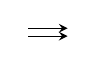
\begin{tikzpicture} \foreach \y in {0.05, 0.15} { \draw [-stealth] (0, \y) -- +(0.5, 0);} \; \end{tikzpicture}}}
\DeclareMathOperator{\leftdoublearrows} {{\; 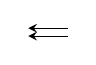
\begin{tikzpicture} \foreach \y in {0.05, 0.15} { \draw [stealth-] (0, \y) -- +(0.5, 0);} \; \end{tikzpicture}}}
\DeclareMathOperator{\righttriplearrows} {{\; 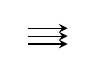
\begin{tikzpicture} \foreach \y in {0, 0.1, 0.2} { \draw [-stealth] (0, \y) -- +(0.5, 0);} \; \end{tikzpicture}}}
\DeclareMathOperator{\lefttriplearrows} {{\; 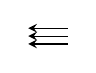
\begin{tikzpicture} \foreach \y in {0, 0.1, 0.2} { \draw [stealth-] (0, \y) -- +(0.5, 0);} \; \end{tikzpicture}}}
\DeclareMathOperator{\rightquadarrows} {{\; 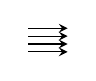
\begin{tikzpicture} \foreach \y in {-0.05, 0.05, 0.15, 0.25} { \draw [-stealth] (0, \y) -- +(0.5, 0);} \; \end{tikzpicture}}}
\DeclareMathOperator{\leftquadarrows} {{\; 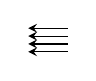
\begin{tikzpicture} \foreach \y in {-0.05, 0.05, 0.15, 0.25} { \draw [stealth-] (0, \y) -- +(0.5, 0);} \; \end{tikzpicture}}}

\newcommand{\ngon}[2][0]{
\begin{tikzpicture}[baseline=-0.5ex,scale=0.8]
\foreach \x in {1, ..., #2}
	\draw (360*\x/#2+#1:.8cm)--(360*\x/#2+#1:.5cm);
\foreach \x in {1, ..., #2}
	\draw (360*\x/#2+#1:.5cm) .. controls +(360*\x/#2+120+#1:.3cm) and +(360*\x/#2+360/#2-120+#1:.3cm) .. (360*\x/#2+360/#2+#1:.5cm);
\end{tikzpicture}
}

\newcommand{\nvertex}[2][0]{
\begin{tikzpicture}[baseline=-0.5ex,scale=0.8]
\foreach \x in {1, ..., #2}
	\draw (360*\x/#2+#1:.8cm)--(0,0);
\end{tikzpicture}
}

\newcommand{\unknot}{
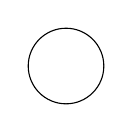
\begin{tikzpicture}[baseline=-0.5ex,scale=0.8]
  \draw (0,0) circle (.6cm);
\end{tikzpicture}
}

\newcommand{\drawI}{ 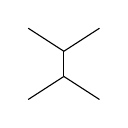
\begin{tikzpicture}[baseline=-0.5ex,scale=0.8]
 	\draw (0,.2) -- (45:.8cm);
 	\draw (0,.2) -- (135:.8cm);
	\draw (0,.2) -- (0,-.2);
 	\draw (0,-.2) -- (-45:.8cm);
 	\draw (0,-.2) -- (-135:.8cm);
\end{tikzpicture}
}

\newcommand{\drawH}{ 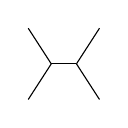
\begin{tikzpicture}[baseline=-0.5ex,rotate=90,scale=0.8]
 	\draw (0,.2) -- (45:.8cm);
 	\draw (0,.2) -- (135:.8cm);
	\draw (0,.2) -- (0,-.2);
 	\draw (0,-.2) -- (-45:.8cm);
 	\draw (0,-.2) -- (-135:.8cm);
\end{tikzpicture}}

\newcommand{\onestrandid}{\begin{tikzpicture}[baseline=-0.5ex,scale=0.8]
	\draw (-.8cm,0)--(.8cm,0);
\end{tikzpicture}}

\newcommand{\twostrandid}{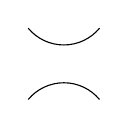
\begin{tikzpicture}[baseline=-0.5ex,scale=0.8]
	\draw (45:.8cm) to [curve through=(90:.3cm)] (135:.8cm);
	\draw (-45:.8cm) to [curve through=(-90:.3cm)] (-135:.8cm);
\end{tikzpicture}}

\newcommand{\cupcap}{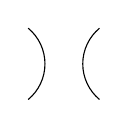
\begin{tikzpicture}[baseline=-0.5ex,rotate=90,scale=0.8]
	\draw (45:.8cm) to [curve through=(90:.3cm)] (135:.8cm);
	\draw (-45:.8cm) to [curve through=(-90:.3cm)] (-135:.8cm);
\end{tikzpicture}}

\newcommand{\symcross}{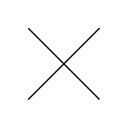
\begin{tikzpicture}[baseline=-0.5ex,scale=0.8]
	\draw (45:.8cm) -- (-135:.8cm);
	\draw (-45:.8cm) -- (135:.8cm);
\end{tikzpicture}}

\newcommand{\braidcross}{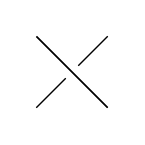
\begin{tikzpicture}[baseline=-0.5ex,scale=0.8]
	\draw (45:.8cm) -- (-135:.8cm);
	\draw[line width=1mm,white,double=black] (-45:.8cm) -- (135:.8cm);
\end{tikzpicture}}


\newcommand{\drawcrossX}{ 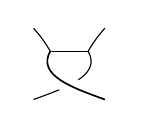
\begin{tikzpicture}[baseline=-0.5ex,scale=0.8,rotate=90]
 	\draw ([out angle=30].2,.3) .. (45:.8cm);
	\draw (.2,.3) -- (.2,-.3);
 	\draw ([out angle=-30].2,-.3) .. (-45:.8cm);
        \draw ([out angle=-150].2,-.3) ..([in angle=-70]135:.8cm);
 	\draw[line width=1mm,white,double=black]
              ([out angle=150].2,.3) .. ([in angle=70]-135:.8cm);
\end{tikzpicture}}

\newcommand{\twist}{
  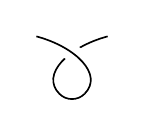
\begin{tikzpicture}[baseline=-0.5ex,scale=0.8]
    \draw[line width=1mm,white,double=black]
       ([out angle=-15]135:.8cm)..([blank=soft]-60:.4cm)..(-120:.4cm)..([in angle=-165]45:.8cm);
    \draw[line width=1mm,white,double=black,use previous Hobby path={invert soft blanks,disjoint}];
  \end{tikzpicture}}

\newcommand{\twistvertex}{
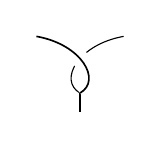
\begin{tikzpicture}[baseline=-0.5ex,scale=0.8]
  \draw (0,-0.5)--(0,-0.8);
  \draw ([out angle=-170]30:0.8cm)..([in angle=150](0,-0.5);
  \draw[line width=1mm,white,double=black]
        ([out angle=-10]150:0.8cm)..([in angle=30](0,-0.5);
\end{tikzpicture}}

\newcommand{\loopvertex}{
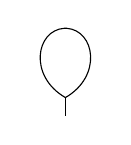
\begin{tikzpicture}[baseline=-0.5ex,scale=0.8]
  \draw (0,-0.5)--(0,-0.8);
  \draw ([out angle=150]0,-0.5)..(-0.02,0.6)..(0.02,0.6)..([in angle=30]0,-0.5);
\end{tikzpicture}
}

\newcommand{\pentagon}{
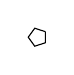
\begin{tikzpicture}[scale=.12,baseline=-2]
\draw (36:1) -- (108:1) -- (180:1) -- (252:1) -- (-36:1) -- (36:1);
\end{tikzpicture}
}

\newcommand{\psq}{
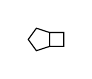
\begin{tikzpicture}[scale=.15,baseline=-2]
\draw (36:1) -- (108:1) -- (180:1) -- (252:1) -- (-36:1) -- (36:1) -- +(1.2,0) -- ($(-36:1)+(1.2,0)$) -- (-36:1);
\end{tikzpicture}
}

\newcommand{\sqsq}{
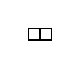
\begin{tikzpicture}[scale=.15]
\draw (0,0) -- (2,0) -- (2,1) -- (0,1) -- cycle (1,0) -- (1,1);
\end{tikzpicture}
}


\begin{document}
\title{Towards the quantum exceptional series}

\author[Morrison]{Scott~Morrison}
\address{Mathematical Sciences Institute, Australian National University}
\email{scott.morrison@anu.edu.au}

\author[Snyder]{Noah~Snyder}
\address{Bloomington, Indiana, USA}
\email{nsnyder1@indiana.edu}

\author[Thurston]{Dylan~P.~Thurston}
\address{Bloomington, Indiana, USA}
\email{dpthurst@indiana.edu}

\begin{abstract}
  We find a single two-parameter skein relation on trivalent graphs,
  the \emph{quantum exceptional relation}, that specializes to a skein
  relation associated to each exceptional Lie algebra (in the adjoint
  representation). If a slight
  strengthening of Deligne's conjecture on the existence of a
  (classical) exceptional series is true, then this relation
  holds for a new two-variable quantum exceptional polynomial, at
  least as a power series near $q=1$. The
  single quantum exceptional relation implies both a deformation of the
  Jacobi relation (true for every Lie algebra) and
 a deformation of the Vogel relation holding for the exceptional series.

  We find a conjectural basis for the space of diagrams with $n$ loose
  ends modulo the quantum exceptional relation for $n \le 7$, with
  dimensions agreeing with the classical computations, and compute
  the matrix of inner products, and the quantum dimensions of idempotents.
  We use the
  skein relation to compute the conjectural quantum exceptional
  polynomial for many knots, in particular
  determining (unconditionally) the values of the quantum polynomials
  for the exceptional Lie algebras on
  these knots. We can compute these for all links of Conway width less 
  than $6$, which includes all prime links with 11 or fewer crossings, and 
  all prime knots with 12 or fewer crossings.
\end{abstract}

%\subjclass[2000]{Primary xxx; Secondary xxx}
%\keywords{}

\maketitle
{ \hypersetup{linkcolor=black}
  \tableofcontents }

\section{Introduction}
\label{sec:introduction}

There are two main 2-variable knot polynomials: the HOMFLY-PT polynomial and
the Kauffman polynomial.  The HOMFLY-PT polynomial interpolates between the
Reshetikhin--Turaev invariants of the standard representations of
$U_q(\mathfrak{gl}_n)$, while the Kauffman polynomial does the same for the
standard representations of quantum $U_q(\mathfrak{o}_n)$ (or, in a slightly
different form, the standard representations of $U_q(\mathfrak{sp}_n)$).  The
two variable nature of these knot polynomials come from the two parameters $n$
and $q$, but we need to replace the discrete parameter $n$ with a continuous
one.   One can think of this process in two steps: first construct a family of
Lie algebra objects in symmetric tensor categories which interpolate between
the $\mathfrak{gl}_n$ yielding something called $\mathfrak{gl}_t$, and second
quantize these Lie algebra objects.   This quantization can be done
systematically using the Kontsevich integral, provided it converges.

Work of Deligne, Cvitanović, Vogel, Cohen-de Man, and others, can be
summarized as a conjecture that there is a third 1-parameter family of Lie
algebra objects in symmetric tensor categories, called the (classical)
exceptional series. This should interpolate between the adjoint
representations of $\mathfrak{sl}_2$, $\mathfrak{sl}_3$, $\mathfrak{so}_8$,
$\mathfrak{g}_2$, $\mathfrak{f}_4$, $\mathfrak{e}_6$, $\mathfrak{e}_7$, and
$\mathfrak{e}_8$ in an appropriate sense.  If this classical exceptional
family exists, we should again expect a quantization yielding a 2-variable
exceptional knot polynomial.  In this paper we give a conjectural skein
theoretic description of this exceptional knot polynomial. In fact, we prove
that these particular skein relations must hold if the exceptional knot
polynomial exists.

We can use these skein relations to do many computations.  In particular, we
are able to calculate the value of this knot polynomial (if it exists!) on all
knots of Conway width 6, which includes all knots of 12 or fewer crossings.
Unconditionally these give the first calculations of the Reshetikhin-Turaev
knot invariants for the exceptional Lie algebras for most of these knots.  
(For 2- and 3-strand torus links and for algebraic/arborescent links such
calculations can already be found by specializing the calculations done by
Mironov--Mkrtchyan--Morozov \cite{MR3491191,MR3475991}.)
For example, we compute the following value for the trefoil for the exceptional
series, and the Reshetikhin-Turaev invariant for $\mathfrak{e}_8$ is given by
setting $v=q^5$ and $w=q^{-1}$.
\begin{multline*}
QES_{\text{reduced}}(\nn{trefoil}) = \\
-v^{24}
\Big(
    \left(w^4 + v^4 w^{-4}\right)\left(-v^{22}+v^{12}+v^{10}-1\right)+\\
    \left(w^2 + v^2 w^{-2}\right)\left(-v^{34}+v^{30}-v^{26}+v^{24}+v^{22}-v^{20}-v^{18}+v^{16}+v^{14}-v^{12}+v^8-v^4\right)+\\
    \left(v^{36}+v^{34}-v^{32}+v^{28}-3 v^{24}-v^{22}+2 v^{20}-v^{16}+v^{14}+2 v^{12}-v^8-v^2-1\right)
    \Big)
\end{multline*}

We are also able to do several other calculations, like giving quantum
dimension formulas for the summands of $\mathfrak{g}^{\otimes 3}$ quantizing
the dimension formulas of Cohen--De Man \cite{MR1381778} in the classical case.
(For the summands of $\mathfrak{g}^{\otimes 2}$ such quantum dimension
formulas were already given by Tuba-Wenzl \cite{MR2132671}.)

In order to state these conjectures and theorems precisely and place them in
their proper context, we have written a  long introduction split into several
subsections.

\subsection{The classical exceptional series}
\label{sec:intro-classical}
We start by giving a skein theoretic
description of the classical exceptional series following Cvitanović, Deligne,
and Vogel.

We begin with the symmetric tensor category of Jacobi
diagrams, $\mathsf{Jac}_d$.

\begin{definition}
Let $R$ be an algebra over $\mathbb{C}$, let $d$ be an element of $R$
and let
$b$ be an invertible element of $R$.  The objects of $\mathsf{Jac}_{R,d,b}$ are
collections of $n$ points on the line and the morphism space from $n$ to $m$
consists of $R$-linear combinations of planar graphs in a rectangle with $n$
boundary points on the bottom, $m$ boundary points at the top, and consisting
of trivalent vertices and $4$-valent symmetric crossings%
\footnote{A symmetric crossing means a crossing as in the symmetric
  group, i.e., not braided.}
modulo planar isotopy, the usual Reidemeister relations
for a symmetric crossing and a trivalent vertex, and the following
circle, lollipop, bigon,
triangle, anti-symmetry, symmetry of the Killing form, and Jacobi relations.
\begin{align}
\label{eq:classical-loop-lollipop}  \unknot \; &= d &  \loopvertex \; &=0 \\
\label{eq:classical-bigon-trigon}  \twogon\; &= b \;\onestrandid  & \threegon\; &= \frac{b}{2} \;\threevertex \\
\label{eq:classical-symmetry-antisymmetry}   \symtwistvertex\; &= - \threevertex & \symtwist\; &= \drawcup
\end{align}
\begin{equation}
\drawI\; - \;\drawH\; + \;\drawsymcrossX\; = 0.
\label{eq:IHX}
\end{equation}
\end{definition}

By rescaling the trivalent vertex, it is easy to see that
$\mathsf{Jac}_{R,d,b}$ is equivalent as a spherical tensor category to
$\mathsf{Jac}_{R,d,bx^2}$ for any invertible $x$ in $R$.  In particular, if $R
= \mathbb{C}$ then $\mathsf{Jac}_{R,d,b}$ does not depend on the choice of
$b$.  A standard normalization is $b=12$.

If $\mathfrak{g}$ is a simple Lie algebra object in a symmetric tensor
category with dimension $d$, by the diagram calculus  the symmetric tensor
category of finite dimensional representations of $\mathfrak{g}$ is the target
of a functor from $\mathsf{Jac}_{R,d,b}$, where we interpret each strand as a
copy of $\mathfrak{g}$, each cup or cap using the Killing form, each trivalent
vertex as the Lie bracket, and each crossing as the usual symmetric braiding.
The skein theory for $\mathsf{Jac}_{R,d,b}$ is somewhat poorly behaved
since the space of $0$-boundary
point diagrams is infinite dimensional.

Cvitanović \cite{MR2418111} and Vogel \cite{MR2769234}
independently observed that the adjoint
representations of the exceptional Lie algebras satisfy another relation, the
\emph{classical exceptional relation}.

\begin{definition}
If $2+d$ is invertible in $R$, let $\mathsf{Exc}_{R,d,b}$ be symmetric tensor category which is the quotient of 
$\mathsf{Jac}_{R,d,b}$ modulo the exceptional relation.
\begin{equation}
\fourgon\; = \frac{b}{6} \left(\;\drawI\; + \;\drawH\; \right)
 + \frac{5}{6}\frac{b^2}{2+d} \left( \;\cupcap\; + \;\twostrandid\; + \;\symcross\; \right)
\label{eq:classical-except}
\end{equation}
\end{definition}

The parameter $d$ is somewhat poorly behaved, and so Deligne instead
introduced a parameter $\lambda$ such that $d = -2
\frac{(\lambda+5)(6-\lambda)}{\lambda(1-\lambda)}$.  This makes sense so long
as $\lambda$ and $1-\lambda$ are invertible in $R$, and such a $\lambda$ can
be found when $2+d$ is invertible and $(2+d)(242+d)$ has a square root in $R$.
Note that $\lambda$ and $1-\lambda$ correspond to the same $d$ and thus to the
same category.  If we normalize $b=12$ then the exceptional relation for
$\mathsf{Exc}_{R,-2   \frac{(\lambda+5)(6-\lambda)}{\lambda(1-\lambda)},12}$
(also written $\mathsf{Exc}_{R,\lambda}$) has the following form.

\begin{equation}
\fourgon\; = 2\left(\;\drawI\; + \;\drawH\;\right)
 - 2\lambda(1-\lambda) \left( \;\cupcap\; + \;\twostrandid\; + \;\symcross\; \right)
\label{eq:classical-except-2}
\end{equation}


\begin{conjecture}[Classical sufficiency]
  \label{conj:class-suffic}
So long as a certain finite set of polynomials in $\lambda$ are invertible,
the space of $n$-boundary point diagrams in $\mathsf{Exc}_{R,\lambda}$ is
finitely generated as an $R$-module for every $n$.  Furthermore,
$\mathsf{Exc}_{R,\lambda}(0,0)$ is generated by the empty diagram,
$\mathsf{Exc}_{R,\lambda}(1,0)$ is the $0$-module,
$\mathsf{Exc}_{R,\lambda}(1,1)$ is spanned by the strand,
$\mathsf{Exc}_{R,\lambda}(2,1)$ is spanned by the trivalent vertex, and
$\mathsf{Exc}_{R,\lambda}(2,2)$ is generated by
\begin{equation}\label{eq:4-box-gen}
  \symcross\;, \; \drawI \;,
  \; \drawH \;, \; \twostrandid \;, \text{ and } \; \cupcap \; .
  \end{equation}
\end{conjecture}

We also conjecture specific spanning sets for $\mathsf{Exc}_{R,\lambda}(n,m)$
for $n+m \leq 6$; see Section~\ref{sec:bases}.

\begin{conjecture}[Classical consistency]
  \label{conj:class-consist}
So long as a certain finite set of polynomials in $\lambda$ are invertible in
$R$, then $R$ injects into $\mathsf{Exc}_{R,\lambda}(0,0)$ as multiples of the
empty diagram.  In particular, any two ways of simplifying the same closed
diagram to give an element of $R$ will give the same element of $R$.
\end{conjecture}

\begin{remark}
  It is possible that classical sufficiency and consistency
  \DPTtodo{Not sufficiency?}
  \NStodo{Added sufficiency.}
  hold even without inverting any polynomials
except for $\lambda$ and $1-\lambda$.  A natural weaker speculation is that one need
only invert elements of the form $r+s\lambda$ for integers $r$ and $s$.
\end{remark}

Note that if $d = -2\frac{(\lambda+5)(6-\lambda)}{\lambda(1-\lambda)}$ is 
invertible in $R$, it follows from classical consistency
that $R$ injects into $\mathsf{Exc}_{R,\lambda}(1,1)$ as multiples of the
strand.  Similarly if $b = 12$ and $d$ are invertible in $R$, it follows from
classical consistency that $R$ injects into $\mathsf{Exc}_{R,\lambda}(2,1)$ as
multiples of the trivalent vertex.  Finally if in addition
$5$, $\lambda-6$, $\lambda-4$, $\lambda+3$, and $\lambda+5$ are invertible
are invertible, then $R^5$ injects into $\mathsf{Exc}_{R,\lambda}(2,2)$ as
linear combinations of the five diagrams in~\eqref{eq:4-box-gen}.
\nn{Is this last statement proved somewhere?}

If both consistency and sufficiency hold, it is also natural to conjecture
that $\mathsf{Exc}_{R,\lambda}(n,m)$ is always a free $R$-module of finite
rank.  When $n+m$ is small this follows from our calculations and the above
conjectures.

\begin{proposition}[Classical specialization]
If Conjecture \ref{conj:class-suffic} holds and $\lambda$ is one of
the values on the left of Table~\ref{tab:lambda-group}, then the
idempotent completion of the quotient of
$\mathsf{Exc}_{\mathbb{C},\lambda}$ by negligible elements is equivalent
to the category of representations of the corresponding group on the
right of Table~\ref{tab:lambda-group}.
\end{proposition}

\begin{table}
  \begin{tabular}{rl}
    \toprule
    $\lambda$ & Supergroup  \\ \midrule
    $-5$ & Trivial group \\
    $-4$ & $\mathrm{SOSp}(1|2)$ \\
    $-3$ & $\mathrm{PSL}(2)$ \\
    $-2$ & $\mathrm{PSL}(3) \rtimes \ZZ/2$ \\
    $-3/2$ & $G_2$  \\
    $-1$ & $\mathrm{PSO}(8) \rtimes S_3$ \\
    $-2/3$ & $F_4$ \\
    $-1/2$ & $E_6 \rtimes \ZZ_2$\\
    $-1/3$ & $E_7$ \\
    $-1/5$ & $E_8$ \\
    \bottomrule
  \end{tabular}
  \caption{Values of $\lambda$ and the supergroup with related category
    representations. In each case, take the Lie group
    with trivial center, semidirect product with its group of outer
    automorphisms.    \label{tab:lambda-group}}
\end{table}

Classical specialization is proved in Section \ref{sec:special-values} following
an idea appearing in \cite{1709.01278}.


\begin{conjecture}[Classical semisimplicity]\label{conj:class-semisimple}
There is a dense open subset $U \subset \mathbb{C}$ so that, for
$\lambda \in U$, the idempotent
completion of $\mathsf{Exc}_{\mathbb{C},\lambda}$ is
semisimple.
\end{conjecture}

We expect that in order for the idempotent completion to be semisimple one
needs to invert infinitely many polynomials.  For example, for the idempotent
completion of $\mathrm{GL}_t$ to be semisimple you need to invert $t-n$ for
every positive integer $n$.  From the dimension formulas of Cohen--De Man and
others, we might speculate that for classical semisimplicity it is
enough to invert $k\lambda-\ell$ for $k, \ell \in \mathbb{Z}$. It
follows from Conjecture~\ref{conj:class-semisimple} that the
idempotent completion of the generic category
$\mathsf{Exc}_{\mathbb{C}(\lambda),\lambda}$ is semisimple.

Deligne's conjecture \cite{MR1378507} is in terms of the existence of
a suitable category. This was
improved by Cohen--De Man \cite{MR1714606} who incorporated the
Cvitanović--Vogel exceptional
relation. They would give a construction of an exceptional series passing
through each of the exceptional Lie algebras.

\begin{conjecture}[Deligne's conjecture]\label{conj:Deligne}
There exists
  \begin{itemize}
  \item a ring $R$ which is a localization of $\mathbb{Q}[\lambda]$ at finitely many polynomials;
  \item a rigid symmetric monoidal category
    $\mathsf{Exc}^D_{R,\lambda}$ where the objects are
    integers and morphism spaces are finitely-generated
    $R$-modules; and
  \item a symmetric monoidal functor $\eval$ from
    $\mathsf{Exc}_{R,\lambda}$ to $\mathsf{Exc}^D_{R,\lambda}$, that
    is the identity on objects and surjective on morphisms.  
  \end{itemize}
   \NStodo{Removed a sentence that Dylan objected to about the image of the trivalent vertex,
    which follows from the below bullet points.}
For any map $\varphi\colon R \rightarrow S$ we can define a base
extension $\mathsf{Exc}^D_{S,\varphi(\lambda)} =
\mathsf{Exc}^D_{R,\lambda} \otimes_\varphi S$.  Furthermore
$\mathsf{Exc}^D$ has the following properties for an open dense subset
$U \subset \mathbb{C}$.
\begin{itemize}
\item The idempotent completion of
  $\mathsf{Exc}^D_{\mathbb{C},\lambda}$ is semisimple for $\lambda \in U$.
\item $\mathsf{Exc}^D_{\mathbb{C},\lambda}(n,m)$ has dimension $1,\allowbreak0,\allowbreak1,\allowbreak1,\allowbreak5,\allowbreak16,\allowbreak80$
for $\lambda \in U$ and $n+m=0,1,2,3,4,5,6$, respectively.
\item If $\lambda$ is one of the special values in
  Table~\ref{tab:lambda-group}, then the idempotent completion of the
  quotient of
  $\mathsf{Exc}^D_{\mathbb{C},\lambda}$ by negligible elements is
  equivalent to the category of representations of the corresponding
  supergroup.
\end{itemize}
\end{conjecture}

Conjecture~\ref{conj:Deligne} follows from
Conjectures~\ref{conj:class-suffic}, \ref{conj:class-consist},
and~\ref{conj:class-semisimple} (using
Proposition~\ref{prop:quant-spec}).
Conjecture~\ref{conj:Deligne} should be
viewed as closer to Conjecture~\ref{conj:class-consist}, since it
doesn't say anything about the kernel of $\eval$;
Conjecture~\ref{conj:class-suffic} says that the classical exceptional
relation is the only skein relation needed to define
$\mathsf{Exc}^D_{R,\lambda}$.

\begin{remark}
  We have learned that Vogel has computational evidence against
  Deligne's conjecture (private communication). Note that it
  is possible for the quantum
  Conjectures~\ref{conj:quant-suffic} and~\ref{conj:quant-consist} to
  hold even if the classical conjectures do not.
\end{remark}

\subsection{Laurent polynomial conventions}

The bulk of this paper deals with quantum versions of the sufficiency and
consistency conjectures.   Before stating these conjectures we fix some
notation for certain Laurent polynomials appearing in our formulas.  On the
one hand, we would like to use formulas that are irreducible as Laurent
polynomials in $v$ and $w$, so that we can easily read off from formulas which
primes need to be inverted.%
\footnote{We avoid the letter $q$, because the relation of our
  parameters to the quantum group parameters is not obvious; see
  Section XXX.}
On the other hand the Laurent polynomials that
occur in our formulas are often even or odd under $v \rightarrow v^{-1}, w
\rightarrow w^{-1}$, so we would also like our formulas to have this symmetry.
So we often combine two irreducible factors into a single expression.  For
example, $v-v^{-1} = v^{-1}(v-1)(v+1) =
(v^{\frac{1}{2}}-v^{-\frac{1}{2}})(v^{\frac{1}{2}}+v^{-\frac{1}{2}})$ but
there is no way to factor it into odd or even Laurent polynomials so we will
leave $v-v^{-1}$ alone in our formulas.  This will never cause any confusion
since any time the irreducible factor $(v-1)$ appears it will have a
corresponding $(v+1)$ factor.

\begin{align*}
[k\lambda + n] &= w^kv^n - w^{-k}v^{-n}\\
\{k\lambda + n\} = \frac{[2k\lambda + 2n]}{[k\lambda + n]} &= w^k v^n + w^{-k} v^{-n}
\end{align*}

\begin{warning}
Unlike with the usual quantum numbers, there is no denominator.
\end{warning}

Note that $\{k\lambda + n\}$ is always irreducible, while $[k\lambda +
n]$ is irreducible iff $k$ and~$n$ are relatively prime. (In
particular, $[n]$ and $[k\lambda]$ are not irreducible for $n,k>1$.)
When
$k=0$ we will generally avoid $[n]$ and instead factor into the following
symmetrized cyclotomic polynomials.  (Strictly speaking we should use
a similar convention for factoring $[k \lambda]$, but this is not needed
in practice.)  Let
\begin{align*}
  \Psi_n &= \prod_{\zeta: \zeta^{n} = \pm 1 \text{ and } \zeta^m \neq \pm 1 \text{ for $m < n$}}
  (v^{\frac{1}{2}}-\zeta v^{-\frac{1}{2}}),\\
  \intertext{or, in terms of the usual cyclotomic polynomials,}
  \Psi_n(v) &= v^{-\varphi(n)} \Phi_{n}(v^2).
\end{align*}
In particular, when $n$ is odd $\Psi_n$ vanishes exactly at primitive
$n$-th and primitive $2n$-th roots of unity, while when $n$ even,
$\Psi_n$ vanishes exactly at primitive $2n$-th roots of unity.
The notation $\{k\lambda + n\}$ can be viewed as another case of this:
for $n$ an odd prime,
$\{n\} = \Psi_{2n}(v)$. For convenience, here are the values of $\Psi_n$ that
appear in this paper.
\begin{align*}
  \Psi_1 & = [1] = v - v^{-1} &
  \Psi_2 & = \{1\} = v + v^{-1}\\
  \Psi_3 & = \frac{[3]}{[1]} = v^2 + 1 + v^{-2}&
  \Psi_4 & = \{2\} = v^2 + v^{-2}\\
  \Psi_5 & = \frac{[5]}{[1]} = v^4 + v^2 + 1 + v^{-2} + v^{-4}&
  \Psi_6 & = \frac{[6][1]}{[3][2]} = v^2 - 1 + v^{-2}\\
  \Psi_7 & = \frac{[7]}{[1]} = v^6 + v^4 + v^2 + 1 + v^{-2} + v^{-4} + v^{-6} &
  \Psi_8 & = \frac{[8]}{[4]} = v^4 + v^{-4} \\
  \Psi_{12} & = \frac{[12][2]}{[6][4]} = v^4 - 1 + v^{-4} \\
\end{align*}
\subsection{Quantum exceptional conjectures}
\label{sec:intro-quantum}
We now turn to our main conjectures.  Our first goal is to give a definition
of a tensor category $\mathsf{QExc}$ which looks like a quantum deformation of
$\mathsf{Exc}$. In particular we need skein relations which deform the Jacobi
relation, the classical exceptional relation, and the symmetric relation
between the overcrossing and undercrossing.  Our specific choices of relations
will be motivated below by our main theorems.

\begin{definition}\label{def:qexc}
Let $R$ be a ring and $v$ and $w$ invertible elements of $R$ such that
$[\lambda]$, $[\lambda-1]$, $\Psi_1$, and $\Psi_6$
are invertible.  Let
$\mathsf{QExc}_{R,v,w}$ be the ribbon category whose objects are collections
of $n$ points on a line, and whose morphisms spaces from $n$ to $m$ consist of
$R$-linear combinations of planar graphs in a rectangle with $n$ boundary
points on the bottom, $m$ boundary points at the top, and consisting of
trivalent vertices and $4$-valent braided crossings modulo planar isotopy, the
usual Reidemeister 2 and 3 relations for a crossing, and the
following circle, lollipop, bigon, triangle, quantum anti-symmetry, and
quantum Killing symmetry relations.

 \begin{equation}
    \label{eq:simple-rels-spec}
  \begin{aligned}
    \unknot\; &= d&\quad
    \loopvertex\;&=0\\[5pt]
      \twogon\;&= b\;\onestrandid&
        \threegon\; &= t\;\threevertex\\[5pt]
    \twistvertex\; &= -v^{6}\;\threevertex&
      \twist\; &= v^{12}\;\drawcup
  \end{aligned}
  \end{equation}
where
\begin{align*}
  d &= -\frac{\Psi_4 [\lambda+5][\lambda-6]}{[\lambda][\lambda-1]}\\
  b &= \{\lambda+2\}\{\lambda-3\}\Psi_3\\
  t &= \Psi_1 \bigl(\Psi_1 \{2\lambda -1\} + (v^4 - v^2 - 1 - v^{-2} + v^{-4})\bigr).
\end{align*}


To these skein relations, we add three more relations:
\begin{itemize}
\item the \emph{quantum exceptional Jacobi relation} (QEJacobi)
\begin{equation}
v^{-3} \;
\drawcrossX
\;+ v \;
\drawI
\; -v^{-1} \;
 \drawH
\;
 - \frac{[\lambda][\lambda-1]}{\Psi_1}
\left[\; \braidcross \;
 + v^{4}\;
\cupcap
\; + v^{-4} \;
 \twostrandid \;
 \right] = 0.\label{eq:quant-except-spec}
\end{equation}

\item the \emph{quantum exceptional square relation} (QESquare)

\begin{equation}
\label{eq:QESquare-w}
\fourgon + \frac{-\Psi_2\Psi_6^2[\lambda][\lambda-1]}{\Psi_1^2} \braidcross + \frac{x_1}{\Psi_1} \drawI + \frac{x_2}{\Psi_1} \drawH + \frac{x_3}{\Psi_1^2} \cupcap + \frac{x_4}{\Psi_1^2} \twostrandid =0
\end{equation}

where the $x_i$ are Laurent polynomials in $v$ and $w$ from Appendix \ref{app:coefficients}.

\item the \emph{quantum exceptional crossing relation} (QECrossing)

\begin{equation}
\label{eq:QECrossing-w}
\braidcross - \invbraidcross + \frac{\Psi_1}{\Psi_6} \left[\; \drawI \; - \; \drawH \; \right] + \frac{\Psi_1 [\lambda][\lambda-1]}{\Psi_6} \left[\; \twostrandid \; - \; \cupcap \; \right] = 0
\end{equation}


\end{itemize}
\end{definition}

Note that if you set $w = v^\lambda$ and take the limit $v \rightarrow 1$
these relations recover the classical Jacobi relation, classical exceptional
relation, and the symmetric crossing relation.  In order to make this
specialization process purely algebraic, we would need to introduce a larger
ring with formal symbols for expressions like $\frac{w-w^{-1}}{v-v^{-1}}$.

\begin{warning}
Although the quantum exceptional Jacobi relation looks like an
analogue of the ordinary Jacobi relation with lower order terms, it is
important to emphasize that it is only the correct analogue of the Jacobi
relation in the exceptional setting.  In particular, it does not hold for
quantizations of non-exceptional Lie algebras.
\end{warning}

We now state our main conjectures.

\begin{conjecture}[Quantum sufficiency]
  \label{conj:quant-suffic}
There is a finite set of polynomials in $v$ and $w$, so that if these
polynomials are invertible in $R$ then the space of $n$-boundary point
diagrams in $\mathsf{QExc}_{R,v,w}$ is finitely generated as an $R$-module for
every $n$.  Furthermore, $\mathsf{QExc}_{R,v,w}(0,0)$ is generated by the
empty diagram, $\mathsf{QExc}_{R,v,w}(0,1)$ is the zero module,
$\mathsf{QExc}_{R,v,w}(1,1)$ is generated by the strand,
$\mathsf{QExc}_{R,v,w}(2,1)$ is generated by the trivalent vertex, and
$\mathsf{QExc}_{R,v,w}(2,2)$ is generated by
$$\braidcross\;, \; \drawI \;, \; \drawH \;, \; \twostrandid \;, \text{and} \; \cupcap \; .$$
\end{conjecture}

We expect that the only additional polynomials you need to invert,
beyond those in Definition~\ref{def:qexc}, are $\Psi_2$, $\Psi_3$, and~$\Psi_5$.
\NStodo{Check that we believe this list of polynomials.}

As before we have conjectured spanning sets for $\mathsf{QExc}_{R,v,w}(n,m)$
for $n+m=0,1,2,3,4,5,6$.

\begin{conjecture}[Quantum consistency]
  \label{conj:quant-consist}
There is a finite set of polynomials in $v$ and $w$, so that if these
polynomials are invertible in $R$ then $R$ injects into
$\mathsf{QExc}_{R,v,w}$ as multiples of the empty diagram.  In particular, any
two ways of applying the above relations to a closed diagram to return a
rational function in $v$ and $w$ will yield the same rational function.
\end{conjecture}

As in the classical case, we again get that if $d$ (resp. $b$) is invertible,
then $R$ also injects into $\mathsf{QExc}_{R,v,w}(1,1)$ (resp.
$\mathsf{QExc}_{R,v,w}(1,2)$) as multiples of the strand (resp. trivalent
vertex).

\begin{proposition}[Quantum specialization]\label{prop:quant-spec}
  If Conjecture \ref{conj:quant-suffic} holds, $\lambda$ is one of
  the values in Table~\ref{tab:lambda-group},
  and $v$ is not a root of unity, then the idempotent completion of
  the quotient of
$\mathsf{QExc}_{\mathbb{C},v,v^\lambda}$ by negligible elements is
equivalent to the category of representations of the quantum version
the corresponding group.
\end{proposition}

Quantum specialization is stated precisely and proved in Section 
\ref{sec:special-values} again following an idea appearing in \cite{1709.01278}. 
In order to make the precise statement we need to give the correspondence
between the parameters $q$ and $v$ which is somewhat subtle.

We expect that quantum specialization this will also be true at roots of unity, 
perhaps excluding some small roots of unity and some parities.

\begin{conjecture}[Quantum semisimplicity]
There is a dense open subset $U \subset \mathbb{C}^2$ for which the idempotent
completion of $\mathsf{QExc}_{\mathbb{C},v,w}$, for $(v,w) \in U$, is
semisimple.
\end{conjecture}

We expect that it's enough to assume that $[k \lambda + \ell]$ is nonzero for all integers $k$ and $\ell$ (in particular, $v$ is not a root of unity).

The following theorems justify the definition of the $\mathsf{QExc}$.  Under
some mild assumptions, any trivalent ribbon category where the $n$-box space
has dimension at most $1,0,1,1,5$ for $n=0,1,2,3,4$ satisfies a version of
relation QEJacobi.  Furthermore, again under some mild assumptions, the
QEJacobi relation implies QESquare and QECrossing.

%With some mild assumptions on the base ring, any skein theory where the $n$-box space has dimension at most $1,0,1,1,5$ for $n=0,1,2,3,4$ satisfies a version of relation~\eqref{eq:quant-except-spec}. %See Theorem~\ref{thm:quant-except} in Section~\ref{sec:relation} for a precise statement.

\begin{definition}
A \emph{trivalent ribbon} category $(\cC, X, \tau)$ is a ribbon category over
$R$ with  an object $X$ such that
the 1-box space is zero, and the 0-, 2-, and 3-box spaces are rank 1 free $R$-modules
generated by the empty diagram, the strand, and a `trivalent vertex' $\tau \in \cC_3$ 
respectively, such that the category is
generated as a ribbon category by $\tau$ and such that the value of the circle
is a non-zero multiple of the empty diagram and the value of the bigon is a
non-zero multiple of the strand.
\end{definition}

Being generated as a ribbon category by $\tau$ is the same as saying that
$\cC$ is generated as a pivotal category by $\tau$ and the crossing.  In
particular, a trivalent ribbon category need not be trivalent in the sense of
\cite{MR3624901} where the trivalent vertex alone is assumed to generate $\cC$ 
as a pivotal category.  Also we have weakened the non-degeneracy condition from
\cite{MR3624901}, replacing it with the assumption that the circle and bigon
are non-zero.

\begin{theorem} \label{thm:Jacobi}
Suppose $(\cC, X, \tau)$ is a trivalent ribbon category over
$\mathbb{C}$ and $\dim{\cC_4} \leq 5$, then there exists $v, \alpha,
b, d, t \in R$ such that the relations in~\eqref{eq:simple-rels-spec}
hold with
\begin{align*}
  [5] b &= - \alpha (d+\{8\}) \\
  t \{2\} &= b-[5] \alpha.
\end{align*}
and
\begin{equation}
v^{-3} \;
\drawcrossX
\;+ v \;
\drawI
\; -v^{-1} \;
 \drawH
\;
 + \alpha
\left[\; \braidcross \;
 + v^{4}\;
\cupcap
\; + v^{-4} \;
 \twostrandid \;
 \right] = 0.\label{eq:quant-except-gen}
\end{equation}
\end{theorem}

If $\dim{\cC_4} = 5$ then relation~\eqref{eq:quant-except-gen} is
unique (up to sending $v \mapsto -v$ and $\alpha \mapsto -\alpha$),
but if $\dim{\cC_4} < 5$ there may be several such relations.

\begin{theorem}\label{thm:square-crossing}
Suppose $(\cC, X, \tau)$ is a trivalent ribbon category over $\mathbb{C}$ with
$\dim{\cC_4} \leq 5$, suppose there exist $v$ and $\alpha$ satisfying the
previous theorem, with $d \neq 0 $, $b \neq 0$, $v^{10} \neq 1$, and $v^{12}
\neq 1$.  Then $\Psi_4 = \{2\}$, $\alpha$, and $b+[3]\alpha$ are
also non-zero, and we have the following relations:
\begin{itemize}
\item
$
  d = -\frac{[5] b}{\alpha} - \{8\} 
$
and
$
  t = \frac{b-[5] \alpha}{\{2\}}.
$
\item

The quantum exceptional square relation:
\begin{equation*} \fourgon + \frac{\alpha \Psi_6 (b+[3]\alpha)}{\Psi_1 \Psi_3 \Psi_4}  \braidcross + \frac{y_1}{\Psi_3 \Psi_4}  \drawI + \frac{y_2}{\Psi_3 \Psi_4}  \drawH + \frac{y_3}{\Psi_1 \Psi_3 \Psi_4} \cupcap + \frac{y_4}{\Psi_1 \Psi_3 \Psi_4} \twostrandid =0
\end{equation*}
where the $y_i$ are Laurent polynomials in $v$ and $w$ given in Appendix \ref{app:coefficients}.
\item
The quantum exceptional crossing relation:
\begin{equation*}
\braidcross - \invbraidcross + \frac{\Psi_1 \Psi_3 \Psi_2 \Psi_4}{b+[3]\alpha} \left[\; \drawI \; - \; \drawH \; \right] - \frac{\Psi_1^2 \Psi_3 \Psi_2 \Psi_4 \alpha}{b+[3]\alpha} \left[\; \twostrandid \; - \; \cupcap \; \right] = 0
\end{equation*}
\end{itemize}

\end{theorem}

We now make a nice change of variables which is motivated by the Kontsevich integral approach.  We first remind the reader of some very elementary mathematics which we nonetheless found quite confusing.

\begin{remark}
Consider the rational change of variables $w= \frac{y}{x+y}$ (retaining $x$ as a variable) which makes sense when $y \neq -x$.  The inverse change of variables is given by the rational function $y = \frac{wx}{1-w}$ which makes sense when $w \neq 1$.  However, in order for them to be inverse we need to calculate that $y$ is equal to
$$\frac{x\frac{y}{x+y}}{1-\frac{y}{x+y}} = \frac{xy}{x}$$ which requires in addition that $x \neq 0$.  By the inverse function theorem this phenomenon happens exactly when $\frac{(x+y)-y}{(x+y)^2} = \partial_w y = 0$.  The same phenomenon also occurs for algebraic functions.
\end{remark}

When $b+[3]\alpha$ is non-zero and the relevant square root exists in $R$ we can make the change of variables
\begin{equation}\label{eq:change-variables}
  w^2 = \frac{v}{2(b+[3]\alpha)}\left(b \{1\} -\alpha [3] \{5\} + \sqrt{-4 (b+[3]\alpha)^2 + (b \{1\} -[3]\{5\}\alpha)^2} \right).
\end{equation}
We see that $\partial_\alpha w^2 = 0$ exactly if $v$ is a $12$th root of
unity, so away from these points the change of variables is invertible, given
by
$$\alpha =  -\frac{b[\lambda][\lambda-1]}{\{\lambda+2\}\{\lambda-3\}\Psi_1\Psi_3}.$$
Note that there are four values of $w$ for each value of $\alpha$.
%% see code2/ChangeOfVariables.nb and code2/ChangeOfVariables2.nb for these calculations

Finally, we observe that upon setting $b =
\{\lambda+2\}\{\lambda-3\}\Psi_3$ these relations are identical to
the formulas in terms of $v,w$ given earlier as Equations
\eqref{eq:QESquare-w} and \eqref{eq:QECrossing-w}.

\begin{corollary}
Suppose $(\cC, X, \tau)$ is a trivalent ribbon category over $\mathbb{C}$ and
suppose there exist $v$ and $\alpha$ such that QEJacobi holds in $\mathbb{C}$
and $d \neq 0 $, $b \neq 0$, $v^{10} \neq 1$, and $v^{12} \neq 1$.  Then there
is a $w \in \mathbb{C}$ and an evaluation functor
$\mathsf{QExc}_{\mathbb{C},v,w} \rightarrow \cC$.
\end{corollary}

This corollary justifies our definition of $\mathsf{QExc}$, since if the
quantum exceptional family exists in any form it would have to satisfy our
quantum exceptional relations.

\subsection{From classical to quantum}
The classical conjectures from Section~\ref{sec:intro-classical} and
the quantum conjectures from Section~\ref{sec:intro-quantum} are
related, but there are not formal implications. From the point of view
of the quantum conjectures, the classical case $v=1$ is in any case
one of the excluded polynomials for any of our concrete results. There
is an implication the other direction: Conjecture~\ref{conj:Deligne}
implies a corresponding quantum conjecture.

\begin{conjecture}[Quantum version of Deligne's conjecture]\label{conj:quant-Deligne}
There exists
  \begin{itemize}
  \item a ring $R$ satisfying the hypotheses of Definition~\ref{def:qexc};
  \item a trivalent ribbon category
    $\mathsf{QExc}^D_{R,v,w}$ where the objects are
    integers and morphism spaces are finitely-generated
    $R$-modules; and
  \item a ribbon functor $\mathrm{Qeval}$ from
    $\mathsf{QExc}_{R,v,w}$ to $\mathsf{QExc}^D_{R,v,w}$, that
    is the identity on objects, surjective on morphisms, and sends
    the trivalent vertex to the trivalent vertex.
  \end{itemize}
As before, we can extend the base. Furthermore
$\mathsf{QExc}^D$ has the following properties for an open subset
$U \subset \mathbb{C}^2$
\begin{itemize}
\item The idempotent completion of
  $\mathsf{QExc}^D_{\mathbb{C},v,w}$ is semisimple for $(v,w) \in U$
\item $\mathsf{QExc}^D_{\mathbb{C},v,w}(n,m)$ has dimension $1,\allowbreak0,\allowbreak1,\allowbreak1,\allowbreak5,\allowbreak16,\allowbreak80$
for $(v,w) \in U$ and $n+m=0,1,2,3,4,5,6$, respectively.
\item If $\lambda$ is one of the special values in
  Table~\ref{tab:lambda-group} and $(v,v^\lambda) \in U$, then the idempotent
  completion of the
  quotient of
  $\mathsf{Exc}^D_{\mathbb{C},\lambda}$ by negligible elements is
  equivalent to the category of representations of the corresponding
  quantum supergroup \footnote{See Section \ref{sec:QGConventions} for quantum 
  group conventions, including what we mean by quantum analogue of an adjoint
  form of a group and of a semidirect product.  See Section \ref{sec:} for the 
  precise statements of the relationship between the parameters $q$ and $v$).}
.\end{itemize}
\NStodo{Dylan left a few todos here, which I think I have to-done}
\end{conjecture}


\begin{theorem}\label{thm:classical-quantum}
  If Conjecture~\ref{conj:Deligne} is true
  for $\mathsf{Exc}_{R,\lambda}$, then
  Conjecture~\ref{conj:quant-Deligne} is true for
  $\mathsf{QExc}_{R((h)),v,w}$ for $v=e^{h/4}$ and $w=e^{\lambda
    h/4}$ as formal Laurent series.
\end{theorem}

This is proved in \S \ref{sec:classical-quantum}.

\subsection{Calculations}
Assuming our main conjectures, we calculate some properties of
$\mathsf{QExc}_{\mathbb{C},v,w}$ and the corresponding $2$-variable knot
polynomial.

First we give conjectural bases for the box spaces up to $n=6$, and check that
these diagrams must be linearly independent.  We unconditionally give a
$16$-dimensional representation of the $5$-strand affine braid group, and an
$80$-dimensional representation of the $6$-strand affine braid group, obtained
from the braid group actions on these $5$- and $6$-boundary point diagrams.

Using this, we give a divide-and-conquer algorithm for computing the
conjectural quantum exception invariant of all links of Conway width 6.
This includes all prime knots of at most 12 crossings, and nearly all prime links of at most 12 crossings,
including many non-algebraic examples.

Note that, unconditionally, these 2-variable knot polynomials must specialize
at particular values of $w$ to give the quantum invariants of the adjoint
representations of the actual Lie algebras.  To our knowledge these are the
first calculations of the quantum knot polynomials of non-torus knots for the
adjoint representations of any of the exceptional Lie algebras, and they are
much more efficient than doing the calculations directly in $U_q(\mathfrak{g})$.
(For torus knots these calculations can be done using the Rosso--Jones formula
\cite{MR1209320}, see \cite{MR3491191}.)

Using our skein relations, we also compute the quantum versions of Cohen--De
Man's formulas for the dimensions of the objects appearing in the third tensor
power of adjoint representation in the exceptional series.

\subsection{Special values}

\nn{Finish writing}

We consider what happens when $v$ specializes to a $10$th or $12$th root of
unity, where some of our skein relations have vanishing denominators. It turns
out that there is still a natural way to define these specializations, and
they recover some interesting examples including the classical exceptional
series, the classical $\mathfrak{g}_2$ series, the classical $\mathfrak{f}_4$
series, Deligne's interpolated symmetric group categories, and a possible new
example related to the ABA free product from \cite{MR3624901}.


\section{Background}
\nn{
Recall:
\begin{itemize}
\item Category of trivalent tangles, perhaps more
\item results from the trivalent paper we need?
\item $SO(3)_{\zeta_{12}}$ plus the
symmetric braiding relation is actually $\mathsf{Rep}(S_3)$ without needing to
semisimplify.  The proof is that R2.5 move implies that the 5-trees simplify
into planar forests.
\item Kontsevich integral
\end{itemize}
}



\subsection{Quantum group conventions}
\label{sec:QGConventions}

If $\mathfrak{g}$ is a complex semisimple Lie algebra, let $U_s(\mathfrak{g})$
denote the Drinfel'd-Jimbo quantum group, and let $\Rep{U_s(\mathfrak{g})}$
denote its ribbon category of representations.

We follow the conventions from \cite{MR2286123}.  See \cite[p. 2]{MR2286123}
for a comprehensive summary of how his conventions line up with those in other
sources. (In particular, our $q$ is the same as both Sawin's $q$ and Lusztig's
$v$.) In particular we have variables $s$ and $q$ and the relation $s^L = q$
where $L$ is the smallest integer such that $L$ times any inner product of
weights is an integer. We always consider Type I finite dimensional representations.
The quantum group itself and its representation theory
only depend on $q$, while the braiding and the ribbon category depend on the
additional choice of $s$.   More generally, for $s$ not a root of unity,
the braiding between irreps $V_\lambda$ and $V_\mu$ depends only on 
$s^{L\langle \lambda, \mu\rangle}$ and so if $\lambda$ is in the
root lattice then the braiding depends only on $q$.

If $s$ is not a root of unity, and $\Lambda'$ is a sublattice of the root lattice,
then the representations whose weights lie in $\Lambda'$ form a tensor
subcategory.  In particular, we can talk about the adjoint subcategory
corresponding to the root lattice.  This subcategory is exactly the subcategory
tensor generated by the adjoint representation.  By the previous paragraph,
the adjoint subcategory as a ribbon tensor category depends only on $q$ and not $s$.
We will abuse notation often by referring to subcategories supported on $\Lambda'$
as quantum versions of the group for which representations supported $\Lambda'$ lift
to representations of the group.   For example, $SO(3)_q$ denotes the adjoint subcategory
of the category of Type I finite dimensional representations of $U_q(\mathbb{su}_2)$.

Finally, if we have a group of automorphisms of the Dynkin diagram,
then this gives a group of braided autoequivalence of the corresponding
ribbon tensor category, and hence we can take the equivariantization by this
action to get a new braided tensor category.  We will again abuse notation
by referring to this as the quantum analogue of the corresponding semidirect
product group.  For example $(PSL(3) \rtimes \mathbb{Z}/2\mathbb{Z})_q$ denotes the
equivariantization of the category of the subcategory  of representations of $U_q(\mathbb{su}_2$
which are supported on the root lattice by the group of Dynkin diagram automorphisms of $A_2$.
This category deforms the category of representations of  the compact group 
$PSL(3) \rtimes \mathbb{Z}/2\mathbb{Z}$.

\begin{remark}
The main source of different $q$ conventions in the literature is that there's
variables $q_i$ for each simple root $\alpha_i$ where the formula for $q_i$
depends on the length of $\alpha_i$.  Our choice of $q$ corresponds to 
$q = q_{\mathrm{short}}$, so that $q_{\mathrm{long}} = q_{\mathrm{short}}^D = q^D$.
It is also common to pick $q_{\mathrm{long}}$ as $q$.   The former convention is natural
if you normalize the inner product on the root space so that short roots have length $2$, while the latter
convention is natural if you normalize the inner product on the root spaces so that long roots have length $2$.
Similarly, if you're studying a family like $\mathbb{so}(2n+1)$, if you uniformly choose $q$ to be $q_{\mathrm{long}}$, 
then $q_n = \sqrt{q}$ and if you specialize to $\mathbb{so}(3)$ you'll end up with a choice of $q$ which is neither
$q_{\mathrm{short}}$ nor $q_{\mathrm{long}}$ (which are equal because there's only one root).

In addition to the conventions for $q$, 
there are many slight variants one can give for the generators and relations, but these typically
do not change the category of representations at generic $q$ at all because they just correspond to rescaling the
choices of $E_i$ and $F_i$ either by scalars or by powers of $K$ and so generate the same algebra $h$-adically.
Because of this rescaling freedom it can sometimes be difficult to work out what $q$ conventions are being used,
because the $[E_i,F_i] = \frac{K_i-K_i^{-1}}{q_i-q_i^{-1}}$ relation changes under rescaling $E_i$ which allows
you to change the denominator on the righthand side.  However, if you look at the Serre relation normalized
so that the leading coefficient is one, then the coefficient of the next term is $-[1-a_{ij}]_{q_i}$, which does not change
under rescaling of $E_i$ and so will tell you what conventions are being used.  For example, in \cite{MR1188811}
the generators and relations for quantum $\mathfrak{so}_{2n+1}$ given use a non-standard normalization of the
final $E_n$, but by looking at the Serre relations we see that $[2]_{q_i} = q+q^{-1}$  for 
$i < n$ but $[3]_{q_n} = q+1+q^{-1}$ so they've chosen $q=q_i=q_{\mathrm{long}}$ and $q_n = q_{\mathrm{long}} = q^{\frac{1}{2}} = q^{\frac{1}{D}}$, so Zhang's $q$ is our $q^2$.
\end{remark}

We use similar conventions for quantum enveloping algebras attached to simple basic Lie superalgebras.  See \cite{MR1266383,MR1892766}, but note that their $q$ is $q_{\mathrm{long}}$ because of the normalization of the inner product.  
Note that in general the quantum enveloping algebras depend not just on the Lie superalgebra but on the choice of simple roots.
For a collection of conventions for simple basic Lie superalgebras see \cite{MR1773773}.  Again, as in the classical case, by the 
quantum analogue of a Lie supergroup, we will mean the appropriate equivariantization of the appropriate subcategory
of representations of the quantized enveloping algebra.  For example, $SOSp(m|2n)_q$ denotes the subcategory of vector representations of $U_q(\mathfrak{so}(m|2n))$, while $OSp(m|2n)_q$ is a $\mathbb{Z}/2\mathbb{Z}$-equivariantization of this category.

In fact, thee only quantum supergroup which we will need to understand in detail is $SOSp(1|2)_q$.
In the next subsection, we will explain how this relates to $SO(3)_q$, and so understanding the general conventions for
quantum supergroups will not be important for this paper.  (Warning: in \cite{MR3624901} we denoted this category $OSp(1|2)_q$,
but this was a poor choice of notation which is not compatible with how we denote categories attached to groups.)


\subsection{Some braided trivalent categories}
In this section, we recall the definitions and fix conventions for some braided tensor categories.

\subsubsection{$SO(3)_q$}
\begin{definition}
When $q$ is not a primitive $8$th root of unity, $SO(3)_q$ be the trivalent ribbon category given by the following relations.

$$  \drawH \; - \; \drawI \; + \frac{b}{q^2+q^{-2}}\; \twostrandid \; -  \frac{b}{q^2+q^{-2}}\; \cupcap = 0$$
$$\braidcross  =  q^{-2} \twostrandid + (q^2 - 1) \cupcap - \frac{(q^2+q^{-2})}{b} \drawI$$
\begin{align*}
    \unknot\; &= q^2+1+q^{-2}&\qquad
      \twist\; &= q^4 \;\drawcup&\qquad
        \twistvertex\; &= -q^2\;\threevertex\\[5pt]
    \loopvertex\;&=0&
      \twogon\;&= b\;\onestrandid&
        \threegon\; &= \frac{q^2-1+q^{-2}}{q^2+q^{-2}} b\;\threevertex
\end{align*}
\end{definition}

As usual we can choose any non-zero value of $b$ without changing the category.  Also sending $q \mapsto -q$ doesn't change the category.  Sending $q \mapsto q^{-1}$ doesn't change the underlying pivotal category but does change the braiding.  The standard normalization of $b$ coming from thinking of $SO(3)_q$ as coming from the second Jones-Wenzl projection is $b = \frac{q^2+q^{-2}}{q+q^{-1}}$. In \cite{MR3624901} we normalize so that $b=1$.

Note that here we have not semisimplified, so when $q$ is a root of unity this category will be degenerate.  For all but a few small roots of unity it will agree with the category of tilting modules for quantum $SO(3)$ defined algebraically. \cite{???}


\subsubsection{$SOSp(1|2)$}
When $q=\pm i$ the diagrammatic category defined in the previous subsection above comes from the supergroup $SOSp(1|2)$ instead of $SO(3)$, see \cite{MR3624901}.  We want to explain this correspondence in more detail to clarify conventions and to explain the relationship between the quantized versions of $SOSp(1|2)_t$ and $SO(3)_q$.

We order the three vectors of a $(1|2)$ super vector spaces so that they go odd, even, odd.  With this ordering, the super transpose on $\mathfrak{gl}(1|2)$ is given by:
$$\begin{pmatrix}
a_{11} & a_{12} & a_{13} \\
a_{21} & a_{22} & a_{23} \\
a_{31} & a_{32} & a_{33}
\end{pmatrix}^{st} = 
\begin{pmatrix}
a_{11} & a_{21} & a_{31} \\
-a_{12} & a_{22} & -a_{32} \\
a_{31} & a_{23} & a_{33} 
\end{pmatrix}
$$

The Lie algebra $\mathfrak{osp}(1|2)$ consists of supermatrices $X \in \mathfrak{gl}(1|2)$ which satisfy $X^{st} \Omega + \Omega X =0$ under the superbracket $[x,y] = xy - (-1)^{|x||y|} yx$, where 
$$\Omega = \begin{pmatrix} 0 & 0 & 1 \\ 0 & 1 & 0 \\ -1 & 0 & 0 \end{pmatrix}$$

An explicit basis of root vectors is given by:
$$H = \begin{pmatrix} 1 & \hspace{.1in}& \hspace{.1in} \\   & 0 &  \\  &  & -1 \end{pmatrix},\,
E_+ = \frac{1}{2} \begin{pmatrix} \hspace{.1in} & 1 & \hspace{.1in} \\   &  & 1 \\  &  &  \end{pmatrix}, \,
E_- = \frac{1}{2} \begin{pmatrix} \hspace{.1in} & \hspace{.1in} & \hspace{.1in} \\ 1  &  &  \\  & -1 &  \end{pmatrix}, \,
J_+ = \begin{pmatrix} \hspace{.1in} & \hspace{.1in} & 1 \\   &  &  \\  & &  \end{pmatrix}, \,
J_- = \begin{pmatrix} \hspace{.1in} & \hspace{.1in} & \hspace{.1in} \\   &  &  \\ 1 & &  \end{pmatrix}.
$$

Here $H, J_+, J_-$ are even and $E_+, E_-$ are odd.  The elements $E_\pm$ are the simple roots, while $J_\pm$ are the root vectors for twice the simple roots.  We have chosen the normalizations to agree with the usual Chevalley-Serre conventions on $H, E_\pm$, and also to satisfy $[J_+,J_-]=H$.  The defining relations that these generators satisfy under the supercommutator are: 
\begin{multline*}[H, E_\pm] = \pm E_\pm, \hspace{.2in} [H, J_\pm] = \pm 2 J_\pm, \hspace{.2in} 
[J_\pm, E_\pm] = 0, \hspace{.2in} [J_+,J_-] = H, \hspace{.2in} [E_+,E_-] = H, \\ [E_\pm,E_\pm] = \pm 2 J_\pm, \hspace{.2in} [J_\pm, E_\mp] = -E_\pm.\end{multline*}

Note that this Lie superalgebra is generated just by $H, E_+, E_-$ without any need for $J_+$ and $J_-$, furthermore using only the relations between $H, E_+, E_-$ gives a presentation of the Lie superalgebra.

Every finite dimensional representation of $\mathfrak{osp}(1|2)$ is semisimple and the irreducible representations are $V_\lambda^\pm$ which have a highest weight vector of weight a non-negative integer $\lambda$ (i.e. $H w = \lambda w$) and parity $\pm$.  Half-integer weights are inconsistent with the superbracket between $E_+$ and $E_-$.  Note that $V_\lambda^\pm$ has graded dimension $(\lambda+1 | \lambda)$ in the positive case and $(\lambda | \lambda+1)$ in the negative case.  The tensor product rules are $W_\lambda^\sigma \otimes W_\mu^\tau =  \bigoplus_{i=|\lambda-\mu}^{\lambda+\mu} W_i^{{-1}^i \sigma \tau}$.

In particular, the defining representation $X = W_1^-$ has graded dimension $(1|2)$ and thus super dimension $-1$, and satisfies
$$X \otimes X \cong 1 \oplus X \oplus W_2^+.$$  In particular, it is a trivalent category with $\dim \Hom(X^{\otimes 2}, X^{\otimes 2}) = 3$. and so must have a skein theory which is $SO(3)_q$ as defined in the previous section for some $q$, and it is easy to see from the dimension that $q = \pm i$.

By \cite{MR2849718,MR3000482} the category of representations of a Lie supergroup can be equivalently described as the category  of super Harish-Chandra pairs, and this is explained for the special case of $OSp$ and $SOSp$ in \cite[\S 7.1]{MR3633307}.  One typically studies a pair $G$ a supergroup and $\varepsilon$ a fixed involution whose conjugation map is the parity automorphism, and denotes $\mathrm{Rep}(G,\varepsilon)$ the category of representations where $\varepsilon$ acts by the parity map.  In particular, $OSp(1|2)$ consists of representations of $\mathbb{osp}(1|2)$ together with a lift to $O(1)\times Sp(2)$ while $SOSp(1|2)$ consists of representations of $\mathbb{osp}(1|2)$ together with a lift to $SO(1)\times Sp(2)$.  We fix $\varepsilon$ to be the diagonal matrix with $1,-1,1$ along the diagonal.  The corresponding category  of representations of $SOSp(1|2)$ is exactly the representations of $\mathbb{osp}(1|2)$ which appear in the tensor powers of the vector representation, while representations of $OSp(1|2)$ are have an additional parity coming from the $O(1) = \mathbb{Z}/2\mathbb{Z}$ which is required to be congruent modulo 2 to the highest weight.  In particular, the invariant spaces for the vector representation $\Hom(V^{\otimes a}, V^{\otimes b}$ for $OSp(1|2)$ vanish unless $a \equiv b \mod 2$ but there's no such restriction for $SOSp(1|2)$.   In particular, $SOSp(1|2)$ is a trivalent category, while $OSp(1|2)$ is a quotient of a BMW category.

We now fix conventions for the quantum version of $\mathbb{osp}(1|2)$.  The $h$-adic version is generated by $H, E_\pm$, with $E_\pm$ odd, subject to the relations $[H,E_\pm] = \pm E_\pm$ and $[E_+,E_-] = \frac{e^{hH}-q^{-hH}}{e^h-e^{-h}}$.  This is a Hopf superalgebra with $\Delta(H) = H \otimes 1 + 1 \otimes H$, $\Delta(E_+) = e^{hH} \otimes E_+ + 1\otimes E_+$, and $\Delta(E_-) = E_-\otimes 1 - e^{-hH} \otimes E_-$.  This has a universal $R$-matrix given by the formula:



Namely it has generators $K, E_\pm$ (again $E_\pm$ are fermionic) which satisfy the relations $K E_\pm K^{-1} = q E_\pm$, $E_+ E_- +  E_- E_+ = \frac{K-K^{-1}}{q-q^{-1}}$.  This has a Hopf superalgebra structure


\subsection{Golden categories}

\begin{definition}
When $q$ is a primitive $5$th or $10$th root of unity then $SO(3)_q$ has an additional quotient called the golden category with the extra relation:
$$\drawI = b \twostrandid - b \frac{1}{q^2+1+q^{-2}} \cupcap.$$

Here $\unknot = q^2+1+q^{-2}$ is $\frac{1\pm \sqrt{5}}{2}$.
\end{definition}

\begin{definition}
For $q$ not a primitive $3$rd, $6$th, $7$th, $14$th, $16$th, or $24$th root of unity, let $(G_2)_q$ be the trivalent ribbon category defined by the following relations.

\begin{align*}
\unknot\; &= \Psi_7(q) \Psi_{12}(q) = q^{10} + q^8 + q^2 + 1 + q^{-2} + q^{-8} + q^{-10}
\end{align*}

\begin{align*}
      \twist\; &= q^{12}  \;\drawcup&\qquad
        \twistvertex\; &= -q^6 \;\threevertex\\[5pt]
    \loopvertex\;&=0&
      \twogon\;&= b\;\onestrandid&
        \threegon\; &= - \frac{\Psi_{6}(q)}{\Psi_{8}(q)} b \;\threevertex
\end{align*}

\begin{align*}
\ngon[45]{4} &=  b \frac{\Psi_4(q)}{\Psi_3(q)  \Psi_{8}(q)} \left(\;\drawI \; +\; \drawH \; \right) +  b^2 \frac{1}{\Psi_3(q)  \Psi_{8}(q)^2} \left(\; \cupcap \; + \; \twostrandid \; \right) \displaybreak[1] \\
\ngon[90]{5} &= - b \frac{1}{\Psi_3(q) \Psi_{8}(q)} \left(\mathfig{0.1}{tree1} + \mathfig{0.1}{tree2} + \mathfig{0.1}{tree3} + \mathfig{0.1}{tree4} + \mathfig{0.1}{tree5} \right) \\
& \qquad - b^2 \frac{1}{\Psi_3(q)^2  \Psi_{8}(q)^2}  \left(\mathfig{0.1}{forest1} + \mathfig{0.1}{forest2} + \mathfig{0.1}{forest3} + \mathfig{0.1}{forest4} + \mathfig{0.1}{forest5}\right),\\
\braidcross  &= \frac{1}{\Psi_2(q)} \left(q^{-3} \twostrandid + q^{3} \cupcap\right) 
	- \frac{1}{b} \frac{\Psi_3(q) \Psi_8(q)}{\Psi_2(q)} 
	\left( q^{-1} \drawH + q \drawI \right).
\end{align*}


\end{definition}

Note that the complicated relation for simplifying pentagons actually follows from the others as in \cite{MR3624901}.

The usual normalization is $b = -\Psi_3(q) \Psi_{8}(q)$ which makes the coefficients of the pentagon relation $+1$ and $-1$ (not quite as in \cite{MR1403861}, which contains an error; see \cite[\S 1.1.3]{MR3624901}) and simplifies the crossing relation.  In \cite{MR3624901} we normalized so that $b=1$.

When $q = \pm i$, we have that $(G_2)_{\pm i}$ has a quotient to $SO(3)_{\pm i}$, which is the value corresponding to $OSp(1|2)$.  Recall that in \cite{MR3624901} we always take the non-degenerate quotient, but we do not do so here, so $(G_2)_{\pm i}$ and $SO(3)_{\pm i}$ denote different trivalent ribbon categories. 

\begin{definition}
For $d \neq 1$, let  $S_{d+1}$ be the trivalent ribbon category given by the following relations.

$$  \drawH \; - \; \drawI \; + \frac{b}{d-1}\; \twostrandid \; -  \frac{b}{d-1}\; \cupcap = 0$$
$$\braidcross  =  \invbraidcross$$
\begin{align*}
    \unknot\; &= d &\qquad
      \twist\; &=  \;\drawcup&\qquad
        \twistvertex\; &=  \;\threevertex\\[5pt]
    \loopvertex\;&=0&
      \twogon\;&= b\;\onestrandid&
        \threegon\; &= b \frac{d-2}{d-1}\;\threevertex
\end{align*}
\end{definition}

The category $S_{d+1}$ is Deligne's interpolated symmetric group category, but instead of the permutation representation as the generator we use the irreducible representation corresponding to the partition $(d,1)$ which is the permutation representation minus the trivial representation.  The endomorphism algebras in this category are called the quasi-partition algebras in \cite{MR3177889}.  Since this example is not the main thrust of this paper we will delay the details of its trivalent ribbon presentation to a future paper.

\begin{warning}
When $d=-1$ our $S_0$ does not agree with Deligne's $S_0$, because in our category the permutation breaks up as a direct sum of the standard and the trivial, whereas for Deligne's the permutation will be a nontrivial extension of the trivial and the standard.  This is closely analogous to what happens for $SO(3)_q$ at $q=\pm i$.  Again we will address this further in a later paper.
\end{warning}

\begin{definition}
$S_{3}$ has a further quotient $\mathrm{Rep}(S_3)$ with the extra relation:
$$\symcross = \frac{1}{b}\drawI + \frac{1}{b}\drawH.$$
\end{definition}

Note that as a pivotal category $\mathrm{Rep}(S_3)$ agrees with the semisimplification of $SO(3)_q$ for $q$ a primitive $12$th root of unity, but the ribbon structures are different (the former is symmetric while the latter is not).  See \nn{add reference to trivalent paper}.






\section{Main results}

Throughout this section $(\cC, X, \tau)$ is a trivalent ribbon category over
$\mathbb{C}$ with $\dim{\cC_4} \leq 5$.  As shown in \cite[Lemma
2.2]{MR3624901}, we have that $X$ is symmetrically self-dual.  As shown in
\cite[Lemma 8.2]{MR3624901}, the trivalent vertex is rotationally invariant.
Thus, using the usual diagram calculus for ribbon categories, we can interpret
$X$ as an unoriented strand, $\tau$ as a trivalent vertex, and then any
trivalent ribbon tangle may be interpreted as a morphism in $\cC$.

\begin{lemma} \label{lem:constants}
  For some numbers $b, d, t, u \in \mathbb{C}$ we have the following relations.
  \DPTtodo{Changed $s$ to $u$ to not conflict with notation used elsewhere.}
  \begin{equation}
    \label{eq:simple-rels}
  \begin{aligned}
    \unknot\; &= d&\qquad
      \twist\; &= u^2\;\drawcup&\qquad
        \twistvertex\; &= -u\;\threevertex\\[5pt]
    \loopvertex\;&=0&
      \twogon\;&= b\;\onestrandid&
        \threegon\; &= t\;\threevertex
  \end{aligned}
  \end{equation}
\end{lemma}

\begin{proof}
All of these follow directly from $\dim \cC_n$ starting $1,0,1,1$ except that
we need to see that the constant for the twisted strand is the square of the
constant for the twisted vertex.  This follows, as in
\cite[Lemma~8.2]{MR3624901}, from the following isotopy:
\begin{equation*}
\overviolin = \rotatedtrivalent. \qedhere
\end{equation*}
\end{proof}

\begin{proposition}\label{prop:Jacobi}
If $\dim \cC_4 \leq 5$, then for some $\beta, \alpha \in \bbC$ and some choice
of~$v \in \bbC$ with $v^6 = u$, we have

\begin{equation}
\beta \left[\; v^{-3} \;
\drawcrossX
\;+ v \;
\drawI
\; -v^{-1} \;
 \drawH
\;\right]
 + \alpha
\left[\; \braidcross \;
 + v^{4}\;
\cupcap
\; + v^{-4} \;
 \twostrandid \;
 \right] = 0.\label{eq:quant-except-init}
 \end{equation}
\end{proposition}

In fact, the conditions we need for the conclusion of
Proposition~\ref{prop:Jacobi} are somewhat weaker than stated. In particular,
we don't need to know the exact dimensions of the $n$-box spaces, just that
certain diagrams are linearly dependent. We do not spell out the details here.

\begin{proof}
  By assumption, the space spanned by the six diagrams
  \[
  \cupcap\;,\qquad\twostrandid\;,\qquad\braidcross\;,
    \qquad\drawI\;,\qquad\drawH\;,\qquad\drawcrossX\;
  \]
  is at most $5$-dimensional.  These six diagrams should be thought
  of as having the symmetries of a tetrahedron (up to framing
  change). To be more precise, we consider the operation~$R$ that cyclically
  rotates three of the input strands:
  \[
  R\left(\,\,\idtangle\,\,\right) = \Rcycle.
  \]
  The operation~$R$ permutes the six diagrams above up to powers of $\pm
  s^k$:
  \begin{align*}
    \begin{tikzpicture}
      \node[inner sep=5pt] (A) at (150:1.4cm) {\cupcap};
      \node[inner sep=5pt] (B) at (30:1.4cm) {\twostrandid};
      \node[inner sep=5pt] (C) at (-90:1.4cm) {\braidcross};
      \draw[|->,bend left=15] (A) to node[above,cdlabel] {s^{-2}} (B);
      \draw[|->,bend left=15] (B) to (C);
      \draw[|->,bend left=15] (C) to (A);
    \end{tikzpicture}&&
    \begin{tikzpicture}
      \node[inner sep=5pt] (D) at (150:1.4cm) {\drawI};
      \node[inner sep=5pt] (E) at (30:1.4cm) {\drawH};
      \node[inner sep=5pt] (F) at (-90:1.4cm) {\drawcrossX};
      \draw[|->,bend left=15] (D) to node[above,cdlabel] {-s^{-1}} (E);
      \draw[|->,bend left=15] (E) to node[below right,cdlabel] {\!\!-s^{-1}} (F);
      \draw[|->,bend left=15] (F) to (D);
    \end{tikzpicture}
  \end{align*}
  (The notation means, for instance, that
  \(
  R\left(\,\raisebox{0.8mm}{\scalebox{0.5}{\cupcap}}\,\right) = s^{-2}\,\,\raisebox{0.8mm}{\scalebox{0.5}{\twostrandid}}\,\,
  \).)
Notice that $R^3$ acts by multiplication by $s^{-2}$. (Indeed,   $R^3$ does
not permute the strands, and is equivalent by   Reidemeister moves to changing
the   framing on the upper-right strand by~$-1$.)  Since $R^{3}$ acts by a
scalar, we have that $R$ acts diagonalizably on the space spanned by these six
diagrams, and in particular on the nonzero space of relations among these six
diagrams in $\cC$.  Thus we must have a relation which is an eigenvector for
the action of $R$ with eigenvalue $\lambda$ with $\lambda^{3} = s^{-2}$.   We
can then pick a square root $\mu$ of $\lambda^{-1}$ such that $\mu^3 = s$, and
then pick $v$ to be either square root of $\mu$.  These are the only two $v$
satisfying $\lambda = v^{-4}$ and $v^6 = s$.
  
Thus we have a relation of
the form of~\eqref{eq:quant-except-init}.
\end{proof}

We now address the case $\beta = 0$.

\begin{lemma} \label{lem:betazero}
  Suppose
  \begin{equation}\label{eq:golden-rel}
    \braidcross \; + v^{4}\;\cupcap\; + v^{-4} \; \twostrandid = 0.
  \end{equation}
  Then $\cC$ is the golden category with $\dim X = \frac{1 + \sqrt{5}}{2}$ or its Galois conjugate.  
\end{lemma}
\begin{proof}
Multiplying by a trivalent vertex we see that $-v^6+v^{-4}=0$, so $v$ is a
$10$th root of unity.  This yields two distinct cases: $v= \pm 1$ or $v = \pm
\zeta_5$ for $\zeta_5$ a fifth root of unity, wlog we take the $+$ sign.

Placing an $H$ on the top of this relation gives a second relation $\psi$
between the six diagrams.  This relation only has one term in the second orbit
of $R$, so $\sum_{i=0}^2 \lambda^i R^i(\psi)$ gives three linearly independent
relations of the above form for the three cube roots of unity $\lambda$.

When $v=1$ the relations we get are:
\begin{align*}
0 &= \braidcross + \twostrandid + \cupcap \\
0 &= \drawcrossX +\drawH + b\cupcap \\
0 &= \drawI - \drawcrossX + b\twostrandid \\
0 &= -\drawH -\drawI + b \braidcross
\end{align*}
Combining the first equation and the last one we see that:
$$\drawI+\drawH = b \twostrandid + b\cupcap.$$
Multiplying by a trivalent vertex we see that $b+t=b$, so $t = 0$.  Pairing
with the square we see that $0 = 2t^2 bd = 2b^3 d$ which is a contradiction
since $b$ and $d$ are non-zero.

When $v$ is a fifth root of unity we get the relations:
\begin{align*}
0 &= \braidcross + v\twostrandid + v^{-1}\cupcap \\
0 &= \drawcrossX +v \drawH + b v^{-1}\cupcap \\
0 &= \drawI - \drawcrossX + b v^{-3} \twostrandid \\
0 &= -v^{-1} \drawH -\drawI + b v^{-3} \braidcross
\end{align*}
Capping off the first equation we see that $v^2 + v +v^{-1}d = 0$, so $d =
-v^2-v^3$ is the Golden ratio or its Galois conjugate.  These four equations
are linearly independent, and by taking the proper linear combinations we see
that:
\begin{align*}
\drawI &=  b\twostrandid + -\frac{b}{d} \cupcap \\
\braidcross &= -v\twostrandid -v^{-1} \cupcap \\
\end{align*}
which are the defining relations of the Golden category.  The values for $v$ and $\alpha$ given in the theorem come from calculating $\sum_{i=0}^2 \lambda^i R^i(\psi)$ for $\lambda$ a cube root of unity.
\end{proof}

\begin{lemma} \label{lem:dandtvalues}
Suppose $\cC$ satisfies QEJacobi for some $v$ and~$\alpha$. Then 
\begin{align}
  [5] b &= - \alpha (d+\{8\})\label{eq:b-rel} \\
  t \{2\} &= b-[5] \alpha.\label{eq:b-t-rel}
\end{align}
Since $b$ and $d$ are nonzero, it follows that $v$ is not a primitive $8$th
root of unity.  If $v$ is also not a 10th root of unity, then $\alpha$ is non-
zero and we have the following formulas.
\begin{align*}
  d &= -\frac{[5] b}{\alpha} - \{8\}   \\
  t  &= \frac{b-[5] \alpha}{\{2\}}.
\end{align*}
\end{lemma}
\begin{proof}
Equation~\eqref{eq:b-rel} follows from closing off QEJacobi with a cap, and
then solving for~$b$. Equation~\eqref{eq:b-t-rel} follows from   closing off
QEJacobi by attaching two ends   to a trivalent vertex, and then solving
for~$t$.
  
If $v$ is a primitive $8$th root of unity, then $0 = t \{2\} = b-[5] \alpha$,
so $b = [5] \alpha$.  Since $b$ is assumed nonzero and $[5]$ is nonzero when
$v$ is a primitive $8$th root of unity, we see that $\alpha = \frac{b}{[5]}$.
Now the first equation becomes $-2 = [5]^2 = -(d+\{8\})=-(d+2)$, which
contradicts $d \neq 0$.   Now $0 \neq [5] b = - \alpha (d+\{8\})$, so $\alpha$
is non-zero and   we can solve for~$d$.
\end{proof}

\begin{proof}[Proof of Theorem \ref{thm:Jacobi}]
By Proposition \ref{prop:Jacobi} and Lemma \ref{lem:betazero} we have that
QEJacobi is satisfied for some $v$ and $\alpha$.  By Lemma \ref{lem:constants}
and Lemma \ref{lem:dandtvalues} we have the other relations.
\end{proof}




\begin{proposition} \label{prop:square-crossing}
  Suppose $\cC$ satisfies QEJacobi for some $v$ and~$\alpha$.
  Then the following equations hold.
\begin{itemize}
  \item The quantum exceptional square relation:
\begin{equation*} [3] \fourgon + \frac{\alpha \Psi_6 (b+[3]\alpha)}{\Psi_4} \braidcross + \frac{y_1 \Psi_1}{\Psi_4} \drawI + \frac{y_2 \Psi_1}{\Psi_4} \drawH + \frac{y_3}{\Psi_4} \cupcap + \frac{y_4}{\Psi_4} \twostrandid =0
\end{equation*}
where the $y_i$ are Laurent polynomials in $v$ and $w$ given in Appendix \ref{app:coefficients}.
  \item
The quantum exceptional crossing relation:
\begin{multline*}
\frac{\Psi_6 \alpha (b+[3]\alpha)}{\Psi_4} \left(\braidcross -
  \invbraidcross \right) + \Psi_1 \Psi_3 \Psi_2 \Psi_6 \alpha \left[\;\drawI \; - \; \drawH \; \right] \\
- \Psi_1^2 \Psi_3 \Psi_2 \Psi_6 \alpha^2 \left[\; \twostrandid \; - \; \cupcap \; \right] = 0.
\end{multline*}
\end{itemize}
 \end{proposition}

\begin{proof}
We attach an $H$-diagram to the QEJacobi relation and then look at the orbit
of this relation under the action of the operator $R$.  Here is the action of
$R$ on the square.
$$
\begin{tikzpicture}
      \node[inner sep=5pt] (A) at (150:1.4cm) {\fourgon};
      \node[inner sep=5pt] (B) at (30:1.4cm) {\twistedsquarehor};
      \node[inner sep=5pt] (C) at (-90:1.4cm) {\twistedsquarever};
      \draw[|->,bend left=15] (A) to (B);
      \draw[|->,bend left=15] (B) to node[right,cdlabel] {v^{-12}} (C);
      \draw[|->,bend left=15] (C) to (A);
\end{tikzpicture}
$$
We attach an $H$ to the bottom of QEJacobi (using that the crossing and $H$
commute) and the apply $R$ and $R^2$.

$$v^{-3} \twistedsquarever + v t \drawI  -v^{-1} \fourgon + \alpha \drawcrossX + \alpha v^4 b \cupcap + \alpha v^{-4} \drawH = 0.$$

$$v^{-3} \fourgon -v^{-5} t \drawH  -v^{-1} \twistedsquarehor + \alpha \drawI + \alpha v^{-8} b \twostrandid - \alpha v^{-10} \drawcrossX = 0.$$

$$v^{-3} \twistedsquarehor +v^{-11} t \drawcrossX  -v^{-13} \twistedsquarever -v^{-6} \alpha \drawH + \alpha v^{-8} b \braidcross - \alpha v^{-10} \drawI = 0.$$

Multiply the first equation by $v^{-2}$, the second by $v^6$, and the third by
$v^8$ and add the three terms, so that all the twisted squares cancel,
yielding:

\begin{multline*}[3] \fourgon +  (t+[1]\alpha)v^{-3} \drawcrossX -(vt +v^{-2}[4]\alpha) \drawH +(v^{-1} t+v^2 [4]\alpha)\drawI \\+ \alpha b \braidcross + \alpha b v^{-2} \twostrandid + \alpha b v^2 \cupcap = 0\end{multline*}

%\begin{align}
%\label{eq:deriving-square-relation}
%\mathfig{0.8}{deriving-square-relation-1} \\
%= \mathfig{0.8}{deriving-square-relation-2}
%\end{align}

We now use the QEJacobi relation to remove the $\drawcrossX$ term, yielding
the QESquare relation.  The QESquare relation minus its 90-degree rotation
gives the QECrossing equation.
\end{proof}

When $v$ is not a $12$th root of unity we can divide by $[3]$,
and if $v$ is not a $10$th root of unity we can divide by $\alpha$.  All that remains in order to prove Theorem
\ref{thm:square-crossing} is to show that when $v$ is not a $10$th or $12$th
root of unity that $b+[3]\alpha$ is non-zero.  Note that if $v$ is not a
$12$th root of unity and $(b+[3]\alpha)$ is zero, then the QECrossing equation
becomes an $SO(3)_q$ relation between the four planar diagrams.  We take a
brief detour to analyze this situation.


\begin{lemma} \label{lem:IequalsH}
Suppose that 
$$\drawI\;- \; \drawH - \frac{1}{d-1} \left(\; \twostrandid - \cupcap \;\right) = 0$$

then one of the following occurs

\begin{itemize}
\item $v$ is a primitive $12$th root of unity.

\item
$\cC$ is a quotient of $SO(3)_q$ for some $q$ with the usual braiding (which
includes the possibility $OSp(1|2)$ when $q= \pm i$)

\item
$\cC$ is  $\mathsf{Rep}(S_3)$.

\end{itemize}
\end{lemma}
\begin{proof}
We apply the tetrahedral symmetry to the relation to get:

$$-s^{-1} \drawH + s^{-1} \drawcrossX -\frac{b}{d-1} \left(\; \braidcross - s^{-2} \twostrandid \; \right) = 0$$
$$s^{-2} \drawcrossX + s^{-1} \drawI -\frac{b}{d-1} \left(\; \cupcap -s^{-2} \braidcross \; \right) = 0.$$

Multiply the first equation by $-s^{-1}$ and then add to the second relation to make the $\raisebox{0.8mm}{\scalebox{0.5}{\drawcrossX}}$ terms vanish. We obtain

$$s^{-1} \drawI + s^{-2} \drawH - \frac{b}{d-1} \left(\cupcap -s^{-2} \braidcross -s^{-1}\braidcross + s^{-3}\braidcross  \right).$$

Unless $s$ is $-1$, this says that $\raisebox{0.8mm}{\scalebox{0.5}{\braidcross}}$ simplifies.  So we split into two cases.

If $\raisebox{0.8mm}{\scalebox{0.5}{\braidcross}}$ simplifies, then we need only solve for all braidings for
$SO(3)_q$, which yields only the usual braiding or when $d=2$ the
additional braiding giving $\Rep(S_3)$ (see \cite[Example 8.6]{MR3624901}).

If $s = -1$, then we want to figure out which sixth roots $v$ of $s$ give a
relation.  That is, we need to figure out which of the rotational eigenvalues
$v^{-4} = \lambda = 1, \omega, \omega^2$ give non-trivial relations.  When
$\lambda = 1$, the sum of the above three relations is trivial.  When $\lambda
= \omega, \omega^2$ then $v$ is a primitive $12$th roof of unity.  (See
Section ??? for further discussion of this case which includes Deligne's
$S_t$.)
\end{proof}

\begin{lemma} \label{lem:bplus3alpha}
Suppose $\cC$ satisfies QEJacobi for some $v$ and $\alpha$ with $v$ not a
primitive $4$th or $12$th root of unity, then $b+[3]\alpha$ is
non-zero.
\end{lemma}
\begin{proof}
If $v$ is a sixth root of unity or if $\alpha$ is zero, then $b+[3]\alpha = b \neq 0$.  So our
assumptions imply that $v$ is not a $12$th root of unity and $\alpha$ is non-zero.
Suppose for the sake of contradiction that $b+[3]\alpha = 0$.  Then by Proposition
\ref{prop:square-crossing} we have that $\cC$ satisfies the assumptions of
Lemma \ref{lem:IequalsH}.  Since $v$ is not a primitive $12$th root of unity, the only
remaining case from Lemma \ref{lem:IequalsH} is that $\cC$ is $SO(3)_q$ with
the standard braiding.  Now a direct calculation shows that $b+[3] \alpha = b
\frac{\Psi_6}{v^4-1+v^{-4}}$ which is non-zero since $v$ is not a
$12$th root of unity, giving a contradiction.
\end{proof}


\begin{proof}[Proof of Theorem \ref{thm:square-crossing}]
Since $v$ is not a $10$th root of unity, by Lemma \ref{lem:dandtvalues} the
equations for $d$ and $t$ hold.  Since $v$ is not a $12$th root of unity $[3]$
is non-zero.  Since $v$ is not a $10$th root of unity $\alpha$ is non-zero.
By Lemma \ref{lem:bplus3alpha} we have that $b+[3]\alpha$ is
nonzero.  Thus we can divide by $[3]$ in the QESquare relation from
Proposition \ref{prop:square-crossing} and divide by $[3](b+[3]\alpha)$ in the
QECrossing relation from Proposition yielding the corresponding relations in
the Theorem \ref{thm:square-crossing}.
\end{proof}


Finally let us motivate the change of variables to $w$ given in the
introduction --- we will see that one of the eigenvalues for the action of
the crossing on the $4$-box space is given by exactly $w^2$.
For this, we need to exclude certain special values of~$v$.
Let $P_{G_2}(q) = q^{10}+q^{8}+q^{2}+1+q^{-2}+q^{-8}+q^{-10}$ be the quantum
dimension of the $7$-dimensional representation of $G_2$.

\begin{lemma} \label{lem:lin-ind-w}
Suppose $\cC$ satisfies QEJacobi for some $v$ and $\alpha$ such that $v$ is
not a $10$th or $12$th root of unity and in addition $d \neq v^6+1+v^{-6}$, $d
\neq P_{G_2}(\zeta_3 v)$, and $d \neq P_{G_2}(\zeta_3^2 v)$, then the
following diagrams are linearly independent:
$$\twostrandid,\quad \cupcap,\quad \drawI,\quad\braidcross,\quad\invbraidcross.$$
\end{lemma}
\begin{proof}
If you pair any two of these diagrams together, the resulting ribbon graph can
be evaluated using the QEJacobi, QESquare, and QECrossing relations.  The
determinant of this matrix (written in terms of $d$ instead of $\alpha$ to
make the formulas simpler) is
\begin{align*}
\frac
{
d^5 v^8 [2][3]^2[6] (d-(v^{6}+1+v^{-6}))^2 (d + \{8\})) (d-P_{G_2}(\zeta_3 v)) (d-P_{G_2}(\zeta_3^2 v))
}
{
[1]^{2}(d + \{4\})^{2}
}.
\end{align*}
%% This is calculated in code/20170522-a-special-case.nb
By our assumptions none of those factors can vanish except possibly
$(d+\{8\})$.  If $d+\{8\} = 0$, then $\frac{[5]b}{\alpha} = 0$ which implies
that $v$ is a $10$th root of unity.
\end{proof}

\begin{remark}
Note that in the cases $d = v^6+1+v^{-6}$, $d=P_{G_2}(\zeta_3 q)$, and 
$d=P_{G_2}(\zeta_3^2 q)$ there are trivalent ribbon categories where the
above diagrams are linearly independent.  Namely, $SO(3)_{v^3}$ satisfies
the quantum exceptional relation with $d = v^6+1+v^{-6}$, while 
$(G_2)_{\zeta_3 q}$

Note that $d = v^6+1+v^{-6}$ corresponds to $SO(3)_{v^3}$, $d=P_{G_2}(\zeta_3 q)$ 
corresponds to $(G_2)_{q}$, and $d=P_{G_2}(\zeta_3^2 q)$ corresponds to
$(G_2)_{q^{-1}}$.  In these examples, the above five diagrams are linearly
dependent.  \NStodo{Check $\zeta$ vs. $\zeta^2$}
\end{remark}

%$(G_2)_q$ satisfies two instances of the QEJacobi relation, $\alpha = b \frac{1-\zeta q^2}{-\zeta^2 q}$ and $v = \zeta q$ for $\zeta$ a primitive cube root of unity.



\begin{lemma}\label{lem:eigenvalues-twist}
If $v$ is not a $10$th or $12$th root of unity, then the crossing acts
diagonalizably on the $4$-box space with eigenvalues $v^{12}$, $-v^{-6}$,
$-1$, $w^2$, and $\frac{v^2}{w^2}$, where $w$ is given by
Equation~\eqref{eq:change-variables}.
\end{lemma}
\begin{proof}
First note that $\frac{1}{d} \raisebox{0.8mm}{\scalebox{0.5}{\cupcap}}$ and $\frac{1}{b} \raisebox{0.8mm}{\scalebox{0.5}{\drawI}}$ are projections
and are eigenvectors for the crossing with eigenvalues $v^{12}$ and
$-v^{-6}$, respectively. We expect three more eigenvalues.
To find them, we look at the action of the crossing
on the image of the projection
$$\pi = \;\twostrandid\; -\frac{1}{d}\;\cupcap\; -\frac{1}{b}\;\drawI\;.$$
Start with QECrossing and multiply by a crossing, then use QEJacobi to remove
the $\raisebox{0.8mm}{\scalebox{0.5}{\drawcrossX}}$ term, and QECrossing to remove the $\raisebox{0.8mm}{\scalebox{0.5}{\drawH}}$ term.  Multiply
again by the crossing and then by $\pi$ to get a cubic equation in the
crossing acting on the image of $\pi$.  By Lemma \ref{lem:lin-ind-w}, the
crossing does not satisfy a quadratic equation, so this cubic polynomial is
the minimal polynomial and its roots are all eigenvalues.  A tedious
calculation shows that the roots of this cubic equation are exactly $-1$,
$w^2$, and $\frac{v^2}{w^2}$.
\end{proof}

\begin{remark}
Recall that the operators $\raisebox{0.8mm}{\scalebox{0.5}{\braidcross}}$ and 
$\raisebox{0.8mm}{\scalebox{0.5}{\drawH}}$ commute.
Thus the eigenvectors for the former (which all have multiplicity $1$
generically) must also be eigenvectors for the latter.  The eigenvalues are
$$\left(v^{12}, b\right), \left(-v^{-6},t\right), \left(-1, [\lambda][\lambda-1]\right), \left(w^2,
\frac{[\lambda][\lambda+2]}{[1]}\right), \text{ and } \left(\frac{v^2}{w^2},
-\frac{[\lambda-1][\lambda-3]}{[1]}\right).$$

There is a nice argument that the above eigenvalues are the only possible
ones.  Namely, suppose $v$ is an eigenvector in the image of $\pi$
with eigenvalues $(\beta, \gamma)$. Multiply $v$ by QEJacobi and reduce
using the known eigenvalues. We find:
$$v^{-3} \beta \gamma -v^{-1} \gamma + \alpha \beta + \alpha v^{-4} = 0.$$
Similarly, multiplying by QECrossing we find:
$$\beta-\beta^{-1} - \frac{\Psi_1 \Psi_3^2 \Psi_2 \Psi_4}{b+[3]\alpha} \gamma - \frac{\Psi_1^2 \Psi_3 \Psi_2 \Psi_4 \alpha}{b+[3]\alpha} = 0.$$
Solving these equations for $\beta$ and $\gamma$ give the list of possible eigenvalues.  We still need some version of Lemma \ref{lem:lin-ind-w} in order to see that all the eigenvalues are realized.
\end{remark}



\section{From the classical to the quantum conjecture}
\label{sec:classical-quantum}
This section is devoted to a proof of
Theorem~\ref{thm:classical-quantum}. Let $\eval$ be the functor from
$\mathsf{Jac}_{R,d,b}$ to $\mathsf{Exc}^D_{R,\lambda}$ given by hypothesis.

The first step is constructing the conjectured functor $\Qeval$ from tangles,
for which the main ingredient is the \emph{Kontsevich integral}~$Z$. The
Kontsevich integral was first defined for unframed knots \cite{MR1318886}, and
later extended to framed trivalent graphs
\cite{MR1473309,MR2304469,MR2661529}. We briefly recall its properties. We
specialize to the case corresponding to the adjoint representation of the Lie
algebra, removing the usual distinction between the two different kinds of
edges.

Let $\mathsf{TriTrangle}$ be the category of framed, unoriented, trivalent
graph tangles. \nn{Maybe this definition should be earlier.} Then, for ring
$R$ containing~$\QQ$ and $d,b \in R$, we have a functor $Z$ from
$\mathsf{TriTangle}$ to $\mathsf{Jac}_{R[[h]],d,b}$. The variable $h$
is used to keep track of
the grading. The functor $Z$ is usually defined as a functor from the category of
parenthesized (non-associative) tangles; to define it as a functor from our
category, where the objects are just integers, for each~$n \ge 3$, pick
arbitrarily a parenthesization of $n$ objects and apply the usual functor.

We will use the following properties of~$Z$.
\begin{enumerate}
\item\label{item:Kontsevich-perturb} $Z(G) = G + O(h)$, where on the
  right hand side we think of the
  underlying trivalent graph of~$G$ as a Jacboi diagram.
\item\label{item:Kontsevich-crossing} On a single crossing, $Z$ takes
  the value
  \begin{equation}
    \label{eq:Kontsevich-crossing}
    Z\biggl(\;\braidcross\;\biggr) =
    \exp\left(\frac{h}{2}\;\drawH\;\right)
    \cdot\; \symcross\;.
  \end{equation}
\end{enumerate}

Then the desired functor $\Qeval$ is the composition of $Z$ with the
classical evaluation $\eval$, with scalars extended to $R[[h]]$. We
then localize at $h$ to take values in the field
$\CC(\lambda)((h))$.
\[
  \mathsf{TriTangle} \overset{Z}{\longrightarrow}
  \mathsf{Jac}_{R[[h]],d,b} {\longrightarrow}
  \mathsf{Exc}_{R[[h]],d,b} \overset{\eval}{\longrightarrow}
  \mathsf{Exc}^D_{R[[h]],d,b}
\]

By hypothesis, the $k$-box spaces of $\mathsf{Except}((h))$ for $k \le 4$
have the required dimensions for a ribbon trivalent category. By
property~\eqref{item:Kontsevich-perturb} of~$Z$,
$\mathsf{Except}((h))$
is generated as a ribbon category over $R((h))$ by a
trivalent vertex.
Furthermore, Equation~\eqref{eq:Kontsevich-crossing} shows that
 that
\begin{align*}
  \Qeval\biggl(\twist\;\biggr) &= e^{hb/2}\eval\biggl(\;\drawcup\;\biggr)\\
  \Qeval\biggl(\! \twistvertex\;\biggr) &= e^{hb/4}\eval\biggl(\threevertex\biggr)
\end{align*}
Comparison with Equation~\eqref{eq:simple-rels-spec} shows that we
should choose $v = e^{hb/24} \in R((h))$. Then by Theorem~\ref{thm:Jacobi}, the
functor $\eval$ satisfies Equation~\eqref{eq:quant-except-gen} for
some value of~$\alpha$. Note that $v^n - 1$ is
invertible for all $n \ne 1$. Thus by Lemma~\ref{lem:bplus3alpha} and
Theorem~\ref{thm:square-crossing} we renormalize~$b$ and make the
change of variables
from Equation~\eqref{eq:change-variables} to get the category
$\mathsf{QExc}_{R((h^t)),v,w}$ for some rational~$t$ and some choice
of~$w$. To identify~$w$ (and see that we can take $t=1$), 
we find the eigenvalues
of the twist operator on the 4-box space.

\DPTtodo{This needs more explanation. Does it go in Background or here?}
\DPTtodo{Double-check these eigenvalues vs $b=12$}
For the classical evaluation $\eval$, the eigenvalues of the crossing
operator and the ladder operator
are $(-1, 6)$, $(-1, 0)$, $(+1, 12)$, $(+1, 2\lambda)$, and
$(+1, 2-2\lambda)$, corresponding to five orthogonal idempotents in the
$(2,2)$-box space. Equation~\eqref{eq:Kontsevich-crossing} then shows
that the corresponding eigenvalues of the twist operator are
$-e^{3h}$, $-1$, $e^{6h}$, $e^{\lambda h}$, and
$e^{(1-\lambda)h}$, respectively.
\nn{Reference to computation of eigenvalues, which is done elsewhere}
On the other hand, by Lemma~\ref{lem:eigenvalues-twist}, the
eigenvalues of the twist
operator in $\mathsf{QExcept}$ are $-v^6$, $-1$, $v^{12}$, $w^2$, and
$v^2/w^2$. To have these two lists of eigenvalues agree, we must
set $v = e^{h/2}$ and $w = e^{\lambda h/2}$.

This completes the proof of Theorem~\ref{thm:classical-quantum}.

\begin{remark}
  Given Conjecture~\ref{conj:class-consist}, to deduce a version of
  Conjecture~\ref{conj:quant-consist} with a non-infinitesimal
  deformation (i.e., valued in, say, complex numbers rather than a
  power series ring), we would have to get control over the
  coefficients in the power series that arise in the functor $\Qeval$
  constructed above. This has been done for the Kontsevich
  integral~$Z$ (XXX: cite). The evaluation algorithm implicit in
  $\eval$ would also have to have computable bounds. \nn{How good} Most
  reasonable evaluation algorithms do give such bounds.
\end{remark}



\subsection{Dimensions}
\nn{Import heuristic arguments for dimensions and eigenvalues from
  \texttt{multiplicities.tex} here, since we need them in the
  Calculations. Say that they are proved later. Talk to Scott before
  doing the import.}

\section{Calculations}
\label{sec:calculations}
\newcommand{\V}{\mathcal{P}}

\subsection{Candidate bases}
\label{sec:bases}
We now consider two candidates bases, $\cB^{\text{braided}}$ and $\cB^{\text
{planar}}$ for each of the spaces $\cP_n$, for $n = 2,3,4,5,6$.
At this point we can only give heuristics for choosing these sets of diagrams;
in the next section we will establish that they are linearly independent, but
it is beyond the scope of this paper to show that they span --- this is
probably at least as hard as showing that the quantum exceptional relation
suffices to evaluate all closed diagrams. Nevertheless they have the expected
sizes, following Cohen--de-Man's claim that the invariant spaces for
$\mathfrak{f}_4$ do not degenerate up to $\cP_6$:
\[
\begin{tabular}{rr}
  \toprule
  $n$ & $\dim \Hom_{\mathfrak{f}_4} (1 \to \mathfrak{f}_4^{\otimes n})$ \\
  \midrule
  0 & 1 \\ 1 & 0 \\ 2 & 1 \\ 3 & 1 \\ 4 & 5 \\ 5 & 16 \\
  6 & 80 \\ 7 & 436 \\ 8 & 2891 \\ 9 & 22248 \\ 10 & 198774 \\
  \bottomrule
\end{tabular}
\]

\newcommand{\diagram}[2]{\mathfig{#1}{graphs/urn_sha1_#2.pdf}}

In order to write our proposed bases compactly, we introduce the following
notations.  Let $D_{*k}$ denote the set of all $k$ inequivalent rotations of the diagram $D$, 
including $D$ itself (when $D$ has $n$ boundary points, $k$ divides $n$).
Let $D_{*k \clubsuit}$ denote the set of the first $k$ counterclockwise rotations of the
diagram $D$ (including $D$ itself), even though these do not exhaust all of the
inequivalent rotations.  In particular, $D_{*1 \clubsuit}$ denotes just the diagram itself.

\DPTtodo{The graphs look good, but the lines should be thicker at this
size}
\SMtodo{unfortunately it's going to be a hassle (an hour's work at least?) to change
the line size, as I've lost a key file}
We define `braided' bases, which use crossings but not squares, as:
\begin{align*}
\cB^{\text{braided}}_0 & = \cB^{\text{planar}}_0 = \left\{ \diagram
{0.1}{8093b057e0fa058603d83e620c4490c7774731e}_{*1}\right\} &
\cB^{\text{braided}}_1 & = \cB^{\text{planar}}_1 = \Bigg\{ \quad \Bigg\} \\
\cB^{\text{braided}}_2 & = \cB^{\text{planar}}_2 = \left\{ \diagram
{0.1}{1f3bf4bb66a4388fb2984eb673be4539182b0256}_{*1} \right\} &
\cB^{\text{braided}}_3 & = \cB^{\text{planar}}_3 = \left\{ \diagram
{0.1}{a7ce858dc75f8bbfee5e1b9837d3d13991f48637}_{*1} \right\}
\end{align*} 
\begin{align*}
\cB^{\text{braided}}_4 & = \left\{ 
  \diagram{0.1}{34a876bb5dae61c3ae047f077a51c37b92ee0789}_{*2},
  \diagram{0.1}{a3a76e07ebde41b851fc63a935929666fca9dcd6}_{*2},
  \diagram{0.1}{d4f429174ebdeb2777a6e5c1f7d726caca7350cd}_{*1\clubsuit}
  \right\} \displaybreak[1]\\
\cB^{\text{braided}}_5 & = \left\{ 
  \diagram{0.1}{e55fafbd03afa4f32c7a584ff8fc14d93149f64e}_{*5},
  \diagram{0.1}{7852166906e0c69e28a717a274dd63ebb2dd14bf}_{*5},
  \diagram{0.1}{25d22603781a5a699a84b26b177c0c228abe0e7a}_{*5},
  \diagram{0.1}{6c16eee9baf0b996fa06ef435e4f0229abade522}_{*1\clubsuit}
  \right\} \displaybreak[1]\\
\cB^{\text{braided}}_6 & = \Bigg\{ 
  \diagram{0.1}{a906b4797b1a0522970b8c97cdb5415a37a14d50}_{*2},
  \diagram{0.1}{1d5fda6573f6e14e019449f842ce86389a666ef3}_{*3},
  \diagram{0.1}{e9f2d2b49d091b0935f5fbd5087a91496a8aea65}_{*6},
  \diagram{0.1}{ae1c9ad2880e168051d75739ff9ac571f47d5418}_{*3},
  \diagram{0.1}{435c40660d57b8d767e9699896b711416756716b}_{*1\clubsuit}, \displaybreak[1] \\
  & \qquad
  \diagram{0.1}{3b78ddd6226e5dcf91391aad721c40afb6d9dce7}_{*3}, 
  \diagram{0.1}{c46af9af2acf5cc00e83232f57fbe67cc3a43b22}_{*6},
  \diagram{0.1}{6b9f6a4077a98d93b7ef68d31d192895cca8de84}_{*6},
  \diagram{0.1}{562a17e80676bec7f61ae4cf18c3cc7c22b9f761}_{*6},
  \diagram{0.1}{2e79238a0fa16c77b7e1b0762abafe754d1f7725}_{*1\clubsuit} \displaybreak[1] \\
  & \qquad
  \diagram{0.1}{392d6cefb5870ced299b7f7140b7253a42e32c47}_{*6},
  \diagram{0.1}{6457494dd06c026dc17137d37534cc940ba96844}_{*6},
  \diagram{0.1}{3b74991ad2c977fa674f4891439a048a05ac0525}_{*3}, 
  \diagram{0.1}{8b6e9125e28b6e81350cac1329d9e353792cf06}_{*3\clubsuit} \displaybreak[1] \\
  & \qquad
  \diagram{0.1}{1baad19a7b800a28edd9aa033244492c73330c5b}_{*3},
  \diagram{0.1}{11a1b489797895c39addff508158f439338f2bd8}_{*3},
  \diagram{0.1}{6aaaa92365996498480cfebe7eeb211bb34dca33}_{*6},
  \diagram{0.1}{82157c05fd8fcf68cf7cd7327cbcee5b7bd885a0}_{*2}, 
  \diagram{0.1}{8dfbd4e54baa5d5755c7a7cef5ae974c6a737cac}_{*6},
  \diagram{0.1}{8a27a57e82333b072ffb4d5b78de022da5c0852b}_{*4\clubsuit}, \displaybreak[1] \\
  & \qquad
  \diagram{0.1}{88b8c27ab39d49cf9e9fdf6be821e0d1c86a5c31}_{*1}
\Bigg\}
\end{align*}

In most of the cases above where we only take some of the rotations of a given
diagram, it is because the other rotations are already isotopic (using
3-dimensional isotopies) to the chosen ones. The exception is that we only
take 4 out of the 6 possible rotations of
$$\diagram{0.1}{8a27a57e82333b072ffb4d5b78de022da5c0852b}.$$

The following heuristic produces these proposed bases.  Consider the classical
setting where the overcrossing and undercrossing are equal.  Now focus on the case
of a graph hose underlying graph is a tree with $k$ leaves.  If you fix the last vertex 
as a root vertex and label the remaining vertices clockwise as $x_1, x_2, \ldots x_{k-1}$, 
then such a diagram can be interpreted as a bracket formula like $[x_2,[x_1, x_3]]$ in
the free Lie algebra on $k-1$ letters.  But due to the Jacobi and antisymmetry relation we should expect these
$(k-1)!$ diagrams to span a space that's smaller than $(k-1)!$ dimensional.  In fact, by 
\cite{???}\NStodo{find a reference}, they span an $(k-2)!$ dimensional space which has as a basis
the diagrams obtained by starting with a fixed tree and permuting $k-2$ of the leaves arbitrarily.

More generally for forests pick a partition of the boundary points into parts with 
at least two elements. For each such partition, and for each part with $k$ elements, 
pick an abstract (unembedded) tree with those $k$ points as the leaves, and form 
the $(k-2)!$ trees (still unembedded) obtained by the symmetric group action on the leaves.
For each such unembedded tree, pick an embedding in the plane which involves as few crossings
as possible.  Finally in the quantum setting we arbitrarily choose over- and under-crossings arbitrarily.

The first line of the proposed basis $\cB^{\text{braided}}_6$ above comes from the partition $6=2+2+2$,
the second line from $6=3+3$, the third line from $6=4+2$, and the fourth line from $6=6$.
(Note that in the first three rows, the `omitted' diagrams marked with $\clubsuit$ are omitted because the additional rotations differ from the included ones just by changing under- and over-crossings, while in the fourth row two diagrams are omitted because we've already reached the expected $(6-2)!$ diagrams.)

Finally, we observe that this procedure only gives 79 elements, and so we throw in the hexagon to get the desired
count of 80.  As one can tell from this step, we do not have a general procedure for producing conjectural
bases (or even the dimensions) when there's more than six boundary diagrams.

The calculations below further allow one to verify that if we add in any natural small diagram not on this list,
the rank of the matrix of pairwise inner products between these diagrams does not increase. (Because we 
have no argument that the inner product is nondegenerate, this observation itself does not lead to new relations.)

We then define corresponding `planar' bases:

\begin{align*}
\cB^{\text{planar}}_4 & = \left\{ 
  \diagram{0.1}{34a876bb5dae61c3ae047f077a51c37b92ee0789}_{*2},
  \diagram{0.1}{a3a76e07ebde41b851fc63a935929666fca9dcd6}_{*2},
  \diagram{0.1}{ac38f78879901186d72dd46debb629071d8a75cc}_{*1}
  \right\} \\
\cB^{\text{planar}}_5 & = \left\{ 
  \diagram{0.1}{e55fafbd03afa4f32c7a584ff8fc14d93149f64e}_{*5},
  \diagram{0.1}{25d22603781a5a699a84b26b177c0c228abe0e7a}_{*5},
\diagram{0.1}{175489e116757578e7d6a10f33f29bd527db673c}_{*1},
\diagram{0.1}{fcc4cb12bd0293b0149f2355e09590e48a13cec3}_{*5}
  \right\} \\
\cB^{\text{planar}}_6 & = \Bigg\{ 
  \diagram{0.1}{a906b4797b1a0522970b8c97cdb5415a37a14d50}_{*2},
  \diagram{0.1}{1d5fda6573f6e14e019449f842ce86389a666ef3}_{*3},
  \diagram{0.1}{51e3597810ca80c60ccbf5ca773dc5f60cc05c26}_{*6},
  \diagram{0.1}{760566cf41c94808243c3091c5f724575b58def2}_{*6},
  \diagram{0.1}{36f1b77eb343f84d3afe9767721856dae4fad1b}_{*3},
  \diagram{0.1}{7faa515ce21febe73dc79066d0a32573cf6951a8}_{*3}, \displaybreak[1] \\
  & \qquad 
  \diagram{0.1}{1baad19a7b800a28edd9aa033244492c73330c5b}_{*3},
  \diagram{0.1}{2ea46d95045afa05d7bd0c8f2dc292ea8d6b000b}_{*3},
  \diagram{0.1}{f357e0b86229ce63736f2ab08989fc2a2f1db2f6}_{*2},
  \diagram{0.1}{d0933ddaf142ecb016df91e1cc0762ab4cc30985}_{*6},
  \diagram{0.1}{a15b7af68d41b9e913156373e080ad2096b76fe}_{*3},
  \diagram{0.1}{cf51f65ba0c14cf15e713f6b099ed1e838e8b36b}_{*6}, \displaybreak[1] \\
  & \qquad 
  \diagram{0.1}{c149b820be2b7d1e7c4b136864ecf03d6d48513c}_{*6},
  \diagram{0.1}{e2072b35dc85bb5c685bc5a889493ee86bf3da8d}_{*6},
  \diagram{0.1}{63ea103b950fa114bda8149d575a29b8eaf74920}_{*6},
  \diagram{0.1}{7de6a0854fa495f044e12f0708481932e9cb121e}_{*1},
  \diagram{0.1}{49bc9767ee6402dfea4c3919f407e7a9dc9d8b59}_{*3},
  \diagram{0.1}{6a3eb98050b8a853009b33fa4bddd634b51b0efd}_{*4\clubsuit}, \displaybreak[1] \\
  & \qquad 
  \diagram{0.1}{b849c60b70156f6044cc8c10b49bd07cd358cde7}_{*3\clubsuit}, 
  \diagram{0.1}{34fabf27c9ebd1f6ece3151ab5f9cde18b1ca09b}_{*1\clubsuit},
  \diagram{0.1}{5004f6fa7f2aa5d72b882308ff24d97dcd8aa047}_{*1\clubsuit}
\Bigg\} 
\end{align*}

One way to understand the relationship between these proposed bases is to observe that there is a bijection between them given
by taking a braided basis diagram, replacing each crossing with a square, and if necessary replacing any adjacent pentagon and square with a single pentagon. We've chosen not to display the diagrams in the order given by this bijection,
but rather by the apparent planar complexity of the diagrams.

\begin{remark}
If you ignore our heuristic which starts with the non-planar basis and instead simply guess an appropriate
number of relatively simple planar diagrams you can easily wind up with a set which is
linearly dependent for the $6$-boundary point diagrams.  In particular, if you replace the 
final five diagrams (involving a hexagon and more than one square)
with the five diagrams $$\left\{\diagram{0.1}{55f53ebaabfb09b3d4727e4b45c3637b0ed8f84c}_{*3}, \diagram{0.1}{c44c9c3e568ce2218151df6d19f09681f6a6e4d8}_{*2}\right\}$$ then those $80$ diagrams are linearly dependent!
\end{remark}

\subsection{Linear independence}
We first check that these bases are linearly independent. 
We have a pairing $\langle - , - \rangle: \V_n \otimes \V_n \to \V_0$ defined
by 
\[
  \langle x, y \rangle =
  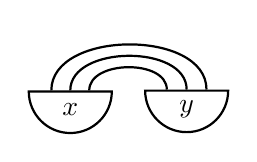
\begin{tikzpicture}[baseline, thick]
    \node[draw, shape=semicircle, shape border rotate=180, minimum size=1.5em] (x) {$x$};
    \node[draw, shape=semicircle, shape border rotate=180, minimum size=1.5em, right=0.5cm of x] (y) {$y$};
    \draw (x.90) to[in=90, out=90] (y.90);
    \draw (x.135) to[in=90, out=90] (y.45);
    \draw (x.45) to[in=90, out=90] (y.135);
  \end{tikzpicture}
\]
and for many (conjecturally all) closed diagrams diagrams in $\V_0$ we can use
the relations to evaluate to a rational function in \(\QQ(v,w)\). Of course,
our basis is far from orthonormal with respect to this pairing!

We first look at the braided bases described above, and find that, up to $n=6$, we can evaluate all matrix entries of $M_n =
\left(\langle e_i, e_j \rangle\right)_{i,j}$. We can then calculate the
determinants of these matrices, obtaining
%% These are calculated in determinants-of-inner-products.nb
\begin{align*}
\det M_3 & = - \frac{
	           \{2\} [\lambda + 5] [\lambda - 6]
             }{
               [\lambda] [\lambda - 1]
             } \\
% -((brk[0, 1] brk[0, 4]^5 brk[0, 5]^3 brk[0, 6]^4 brk[1, -6]^5 brk[
%       1, -4]^2 brk[1, -3] brk[1, 2] brk[1, 3]^2 brk[1, 5]^5 brk[
%       3, -6] brk[3, 3])/(brk[0, 2]^7 brk[0, 3]^4 brk[1, -2] brk[
%       1, -1]^8 brk[1, 0]^8 brk[1, 1] brk[2, -6] brk[2, 4]))
\det M_4 & = \frac{
              [1] [4]^5 [5]^3 [6]^4 [\lambda - 6]^5 [\lambda - 4]^2 [\lambda - 3] [\lambda + 2]
              [\lambda + 3]^2 [\lambda + 5]^5 [3\lambda - 6] [3\lambda + 3]
             }{
              [2]^7 [3]^4 [\lambda - 2] [\lambda - 1]^8 [\lambda]^8 [\lambda + 1]
              [2 \lambda - 6] [2\lambda + 4]
             } \displaybreak[1]\\
% -((brk[0, 1]^7 brk[0, 4]^16 brk[0, 5]^13 brk[0, 6]^20 brk[
%       1, -6]^16 brk[1, -4]^10 brk[1, -3]^12 brk[1, 2]^12 brk[1, 
%       3]^10 brk[1, 5]^16 brk[3, -6]^6 brk[3, 3]^6 brk[4, -6] brk[4, 
%       2])/(v^2 brk[0, 2]^24 brk[0, 3]^32 brk[1, -2]^6 brk[
%       1, -1]^26 brk[1, 0]^26 brk[1, 1]^6 brk[2, -6]^12 brk[2, -3] brk[
%       2, 1] brk[2, 4]^12))
\det M_5 & = 
             \frac{
              [1]^7 [4]^{16} [5]^{13} [6]^{20} [\lambda - 6]^{16} [\lambda - 4]^{10} 
              [\lambda - 3]^{12} [\lambda + 2]^{12}
              [\lambda + 3]^{10} [\lambda + 5]^{16} 
             }{
              v^2 [2]^{24} [3]^{32} [\lambda - 2]^{6} [\lambda - 1]^{26} [\lambda]^{26} [\lambda + 1]^6
              [2 \lambda - 6]^{12} [2\lambda - 3] [2\lambda + 1] [2\lambda + 4]^{12}
             } \times \\
         & \qquad \times [3\lambda - 6]^6 [3\lambda + 3]^6
              [4 \lambda - 6] [4\lambda + 2] \displaybreak[1]\\
\det M_6 & = \frac{
              -v^{12} [1]^{67} [4]^{80} [5]^{75} [6]^{165} [\lambda - 6]^{80} [\lambda - 5]^{15} [\lambda - 4]^{65} [\lambda - 3]^{112} [\lambda + 3]^{65} [\lambda + 4]^{15} [\lambda + 5]^{80} 
             }{
               [2]^{151} [3]^{268} [\lambda - 2]^{50} [\lambda - 1]^{150} [\lambda]^{150} [\lambda + 1]^{50} [2\lambda - 6]^{107} [2\lambda - 3]^{10} [2\lambda + 1]^{10} [2\lambda + 4]^{107}
             } \times \\
         & \qquad \times [2 \lambda - 4]^5 [2\lambda + 2]^5 [3\lambda - 6]^{45} [3\lambda + 3]^{45} [4 \lambda - 6]^{10} [4\lambda + 2]^{10} [5\lambda - 6] [5\lambda + 1].
\end{align*}



In particular, we see that $\det M_4$ vanishes when $v^k = 1$ for
$k=1,2,4,5,8,10$, or $12$, or when $w = \pm v^k$ for $k=-5,-3,4,6$, or when
$v^4 \pm v^2 w + w^2 = 0$ (equivalently, $w = \zeta v^{-1}$ for $\zeta$ a
primitive 3rd or 6th root of unity) or $1 \pm v w + v^2 w^2 = 0$
(equivalently, $w = \zeta v^2$ for $\zeta$ a primitive 3rd or 6th root of
unity). Then, $\det M_5$ vanishes at all the same places, and additionally at
$v^6 + w^4 = 0$ and $1 + v^2 w^4 = 0$. Finally $\det M_6$ vanishes everywhere $\det
M_5$ does, and also at $w = \pm v^k$ for $k=-4,-2,3,5$, $w = \pm i v^k$ for
$k=-1,2$, $v = \pm w^{-5}$ and $w^5 \pm v^6 = 0$.

In fact, the components of $\det M_4 = 0$ and $\det M_5$ are explained by smaller categories
which we already know about, or degenerate cases. \nn{appropriate reference
elsewhere in the paper for the $v^k = 1$ cases} At $w = \pm v^{-5}$ and $w =
\pm v^6$, we see that $d=0$, so any quotient would be degenerate. At $w = \pm
v^{-3}$ and $w = \pm v^4$, we recover the $SO(3)_q$ categories \nn{details?}.
At $w = \zeta v^2$, with $\zeta$ a primitive 3rd or 6th root, we obtain
$(G_2)_q$ \nn{details}. \nn{What about $w = \zeta v^{-1}$?}  
For $\det M_5$ the curves $v^6 + w^4 = 0$ and $1 + v^2 w^4 = 0$ correspond to
quantum $E_6$.

Although it may appear that new factors are appearing in the
denominators as we look at $\det M_3, \det M_4, \det M_5, $ and $\det
M_6$, one should recall that the bracket polynomials $[a \lambda + b]$
are not generally irreducible. The
irreducible factors appearing in the denominator after cancellation
remain the denominators \nn{already} introduced: $\det M_4$ has poles
at $w=\pm1, v=\pm w, v^6+w^2 = 0$, and $1+v^4w^2 = 0$,
then $\det M_5$ has additional poles at $w=0, 1\pm v + v^2 = 0$, and $\det M_6$
has another pole at $v = \pm 1$.


\subsection{Matrices for operations}
In this section, we obtain matrices for the braiding and rotation operators on
 $\V_n$, `relative to' $\cB^{\text{braided}}$ described above.
We have to be careful here, as we don't know that $\cB^{\text{braided}}$
actually spans $\V_n$, or even that the braiding and rotation operators map
the span of $\cB^{\text{braided}}$ to itself.

Showing the braiding and rotation  preserve the span of $\cB^{\text{braided}}$ 
is much more tractable than proving our main conjectures; we would only need to
apply braiding or rotation to each element, and show that it
is possible to use the relations to rewrite the result as a linear combination
of elements of $\cB^{\text{braided}}$.  For practical computational reasons we 
take a slightly different approach,
computing via pairings the matrix which \emph{would} be associated to each of the
operations \emph{if} $\cB^{\text{braided}}$ really were a basis, and then
verifying that these matrices satisfy the expected properties.

Given an operator $T: \V_n \to \V_m$, if the $\cB^{\text{braided}}_n$
are bases, the associated matrix for $T$ would be $AM_m^{-1}$, where
$A = \left(\langle T e_i, e_j \rangle\right)_{i,j}$.
Rather unfortunately inverting the matrix $M_6$ is computationally
infeasible. (Recall that arithmetic over $\QQ(v,w)$ may be quite inefficient!)

We find, nevertheless, that for $T$ any of
\begin{align*}
  (\rho_n : \V_n \to \V_n) & = 
    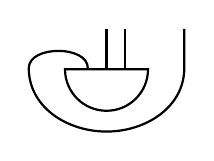
\begin{tikzpicture}[baseline, thick]
      \node[draw, shape=semicircle, shape border rotate=180, minimum size=1.5em] (x) {};
      \draw (x.90) -- ++(0,0.5);
      \draw (x.45) -- ++(0,0.5);
      \draw (x.135) to[in=90, out=90] ++(-0.75,0) 
                     to[in=180,out=-90] ($(x.-90)+(0,-0.25)$) 
                     to[out=0,in=-90] ($(x.45)+(0.75,0)$)
                     -- ++(0,0.5);
    \end{tikzpicture} &
  (\beta_n : \V_n \to \V_n) & = 
    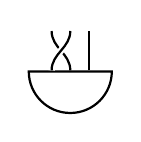
\begin{tikzpicture}[baseline, thick]
      \node[draw, shape=semicircle, shape border rotate=180, minimum size=1.5em] (x) {};
      \draw (x.45) -- ++(0,0.5);
      \draw (x.90) to[out=90,in=-90] ($(x.135)+(0,0.5)$);
      \draw[knot] (x.135) to[out=90,in=-90] ($(x.90)+(0,0.5)$);
    \end{tikzpicture} 
  \displaybreak[1] \\
  (\cap_n : \V_n \to \V_{n-2}) & = 
    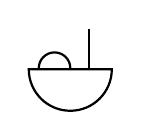
\begin{tikzpicture}[baseline, thick]
      \node[draw, shape=semicircle, shape border rotate=180, minimum size=1.5em] (x) {};
      \draw (x.45) -- ++(0,0.5);
      \draw (x.90) arc (0:180:0.2);
    \end{tikzpicture}
  &
  (\cup_{n-2} : \V_{n-2} \to \V_{n}) & = 
    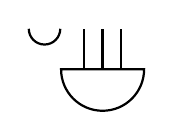
\begin{tikzpicture}[baseline, thick]
      \node[draw, shape=semicircle, shape border rotate=180, minimum size=1.5em] (x) {};
      \draw (x.90) -- ++(0,0.5);
      \draw (x.45) -- ++(0,0.5);
      \draw (x.135) -- ++(0,0.5);
      \draw ($(x.135)+(0,0.5)+(-0.3,0)$) arc (0:-180:0.2);
    \end{tikzpicture}
  \displaybreak[1] \\
  (\fork_{n-1} : \V_{n-1} \to \V_{n}) & = 
    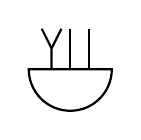
\begin{tikzpicture}[baseline, thick]
      \node[draw, shape=semicircle, shape border rotate=180, minimum size=1.5em] (x) {};
      \draw (x.90) -- ++(0,0.5);
      \draw (x.45) -- ++(0,0.5);
      \draw (x.135) -- ++(0,0.25) -- ++(0.125,0.25);
      \draw    ($(x.135)+(0,0.25)$) -- ++(-0.125,0.25);
    \end{tikzpicture}
  &
  (\fuse_n : \V_n \to \V_{n-1}) & = 
    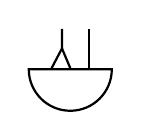
\begin{tikzpicture}[baseline, thick]
      \node[draw, shape=semicircle, shape border rotate=180, minimum size=1.5em] (x) {};
      \draw (x.45) -- ++(0,0.5);
      \draw (x.90) -- ($(x.114)+(0,0.25)$);
      \draw (x.135) -- ($(x.114)+(0,0.25)$) -- ++(0,0.25);
    \end{tikzpicture}
  \\
  (H_n : \V_n \to \V_n) & = 
    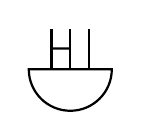
\begin{tikzpicture}[baseline, thick]
      \node[draw, shape=semicircle, shape border rotate=180, minimum size=1.5em] (x) {};
      \draw (x.45) -- ++(0,0.5);
      \draw (x.90) -- ++(0,0.5);
      \draw (x.135) -- ++(0,0.5);
      \draw ($(x.90)+(0,0.25)$) -- ($(x.135)+(0,0.25)$);
    \end{tikzpicture}
\end{align*}
with $n \leq 6$,
we can evaluate all of the matrix entries of $A$ as rational functions.
(Even though $H_n = \rho_{n}^{-1} \fuse_n \rho_{n+1} \fork_n$, we can not
use this to compute $H_6$ as we would need to know $\rho_7$ and $\fuse_7$.)

Even though directly inverting $M$ is infeasible, we find that we can
calculate the product $A M^{-1}$ in each case. (Nevertheless this remains a
difficult calculation ---  we use some tricks, calculating the product at
various specialisations of the variables and then using interpolation, finally
verifying our answer by multiplying by $M$.)

Explicit matrices are available with the {\tt arXiv} sources of this article,
as the files $$\text{{\small\tt matrices/n-box-OP-matrix.m}},$$ where $n \leq
6$, and {\tt OP} is one of {\tt rotation}, {\tt braiding}, {\tt inverse-%
braiding}, {\tt cup}, {\tt cap}, {\tt fork}, {\tt fuse}, {\tt H}.  The
matrices are written in terms of the variables $d, v$.


\subsection{Representations of braid groups}
The affine $n$-strand braid group has generators $\rho$ and $\beta$, with
relations $\rho^n = 1$, $\beta \rho^\pm \beta \rho^\mp \beta = \rho^\pm \beta
\rho^\mp \beta \rho^\pm \beta \rho^\mp$, and $\beta \rho^i \beta \rho^{-i} =
\rho^i \beta \rho^ {-i} \beta$ for all $i = 2, \ldots, n-2$.

At this point, we may verify that the matrices $\rho = \rho_n$ and $\beta =
\beta_n$ provide a representation of the affine $n$-strand braid group merely
by multiplying out the matrices.

\begin{lemma}
The matrices described in the previous section give a representation of the affine $n$-strand braid group for $3 \leq n \leq 6$.
\end{lemma}


\subsection{Idempotents in the 6-box space}

In order to analyze the 6-box space, we compute in the span of $\cB^{\text{braided}}_6$ the simultaneous eigenvectors for the commuting operators
\begin{align*}
Tw_3 = (\beta_6 \rho_6 \beta_6 \rho_6^{-1})^3 & = \begin{tikzpicture}[baseline, thick]
      \braid[number of strands=6, xscale=0.35, yscale=-0.35] (braid) a_1 a_2 a_1 a_2 a_1 a_2;
      \node[draw, shape=semicircle, shape border rotate=180, minimum size=2.5em] at ($(braid-1-s)+(0.88,-0.45)$) (x) {};
    \end{tikzpicture}
&
\beta_6 & = \begin{tikzpicture}[baseline, thick]
      \braid[number of strands=6, xscale=0.35, yscale=-0.35] (braid) a_1;
      \node[draw, shape=semicircle, shape border rotate=180, minimum size=2.5em] at ($(braid-1-s)+(0.88,-0.45)$) (x) {};
    \end{tikzpicture}
&
\rho_6^4 \beta_6 \rho_6^{-4} & = \begin{tikzpicture}[baseline, thick]
      \braid[number of strands=6, xscale=0.35, yscale=-0.35] (braid) a_5;
      \node[draw, shape=semicircle, shape border rotate=180, minimum size=2.5em] at ($(braid-1-s)+(0.88,-0.45)$) (x) {};
    \end{tikzpicture}
\end{align*}

The characteristic polynomial of $Tw_3$ is 
\begin{align*}
w^{-72}
\left(v^{36}-\lambda \right)
\left(v^{24}-\lambda \right)^{25}
\left(v^{12}-\lambda \right)^{16}  
& \left(v^{12} w^4-\lambda \right)^9
\left(v^{16}-\lambda  w^4\right)^9 \\
\left(1 - \lambda\right)
\left(w^{12}-\lambda \right) 
&\left(v^{12}-\lambda  w^{12}\right)
\left(v^4-\lambda \right)^9 
\left(w^6-\lambda \right)^4  
\left(v^6-\lambda  w^6\right)^4, 
\end{align*}

By a direct calculation of nullspaces we find this triple of operators has distinct eigenvalues, as shown in Table \ref{tab:braid-gen}, so we obtain 80 eigenvectors, each of which is uniqely determined up to scale. 
\begin{table}
  \centering
  \begin{tabular}{ccccccc}
    \toprule
    &&\multicolumn{5}{c}{$\beta_6$ and $\rho_6^4 \beta_6 \rho_6^{-4}$ eigenvalues} \\ \cmidrule(l){3-7}
   $\Tw_3$ & Mult & $v^{12}$ & $-v^{-6}$ & $-1$ & $w^2$ & $v^2w^{-2}$ \\
    \midrule
   $v^{36}$        & $1$  & - & 1 & - & - & - \\[2pt]
   $v^{24}$        & $25$ & 1 & 1 & 1 & 1 & 1 \\[2pt]
   $v^{12}$        & $16$ & - & 1 & 1 & 1 & 1 \\[2pt]
   $v^{12}w^4$     & $9$  & - & 1 & 1 & 1 & - \\[2pt]
   $v^{16}w^{-4}$  & $9$  & - & 1 & 1 & - & 1 \\[2pt]
   $1$             & $1$  & - & - & 1 & - & - \\[2pt]
   $w^{12}$        & $1$  & - & - & - & 1 & - \\[2pt]
   $v^{12}w^{-12}$ & $1$  & - & - & - & - & 1 \\[2pt]
   $v^4$           & $9$  & - & - & 1 & 1 & 1 \\[2pt]
   $w^6$           & $4$  & - & - & 1 & 1 & - \\[2pt]
   $v^6w^{-6}$     & $4$  & - & - & 1 & - & 1 \\
    \bottomrule
  \end{tabular}
  \medskip
  \caption{Decomposition of the 6-box space into eigenspaces of the full twist and braid generators}\label{tab:braid-gen}
\end{table}

In fact, writing a joint eigenvector with eigenvalues $x,y,z$ as $v_{x,y,z}$, we see that
they must provide matrix units (up to some scalars) with respect to the multiplication,
even though we can't verify this directly.
Certainly $v_{x,y,z} \bullet v_{x',y',z'} = 0$ unless $x = x'$, since the full twist $Tw_3$ is central.
Moreover as
\begin{align*}
\rho_6^4 \beta_6 \rho_6^{-4}(v_{x,y,z}) \bullet v_{x,y',z'} 
  & = v_{x,y,z} \bullet \beta_6 (v_{x,y',z'})
\end{align*}
and all the joint eigenspaces are one dimensional, we must have $v_{x,y,z} \bullet v_{x,y',z'}$ a
multiple of $\delta_{z,y'} v_{x,y,z'}$.



In particular, the $v_{x,y,y}$ (when non-zero) are minimal idempotents (up to scale), and picking one
such eigenvalue $y_x$ for each eigenvalue $x$ of $Tw_3$ so $v_{x,y_x,y_x} \neq 0$, these give a complete
set of representatives of the minimal idempotents

We can compute the quantum traces of these idempotents, as
$$\frac{\langle v_{x,y,y}, id \rangle^2}{\langle v_{x,y,y}, v_{x,y,y} \rangle}$$
(this quantity is homogeneous, so we may assume that we have picked $v_{x,y,y}$ to actually be an idempotent, and then $\langle v_{x,y,y}, v_{x,y,y} \rangle = \langle v_{x,y,y}, id \rangle$ so after
cancelling we have the quantum dimension).

We obtain the dimensions displayed in Table \ref{tab:quantum-dimensions},
and one can check that after setting $v=1$ (achieved by replacing $[k\lambda+l]$ with $k\lambda+l$) these agree
with the tables in \cite[p.431]{MR1381778}.

\begin{table}
  \centering
  \begin{tabular}{ccc}
    \toprule
   eigenvalue of $\Tw_3$ & representation & quantum dimension \\
    \midrule
   $v^{36}$        & $1$     & $1$ \\[2pt]
   $v^{24}$        & $X_1$   & $-\frac{[4][\lambda+5][\lambda-6]}{[2][\lambda][\lambda-1]}$ \\[2pt]
   $v^{12}$        & $X_2$   & $\frac{[5][\lambda+5][\lambda+3][\lambda-4][\lambda-6][2\lambda+4][2\lambda-6]}{[1][\lambda+2][\lambda][\lambda-1][\lambda-3][2\lambda][2\lambda-2]}$ \\[2pt]
   $v^{12}w^4$     & $Y_2$   & $-\frac{[4][5][6][\lambda+5][\lambda-4][3\lambda-6]}{[2][\lambda][\lambda-1][\lambda-2][2\lambda][2\lambda-1]}$ \\[2pt]
   $v^{16}w^{-4}$  & $Y_2^*$ & $-\frac{[4][5][6][\lambda-6][\lambda+3][3\lambda+3]}{[2][\lambda-1][\lambda][\lambda+1][2\lambda-2][2\lambda-1]}$ \\[2pt]
   $1$             & $X_3$   & $- \frac{[4][5][\lambda+5][\lambda+4][\lambda-5][\lambda-6][2\lambda+4][2\lambda-6][3\lambda+3][3\lambda-6]}{[1][2][\lambda+1][\lambda][\lambda-1][\lambda-2][2\lambda][2\lambda-2][3\lambda][3\lambda-3]}$ \\[2pt]
   $w^{12}$        & $Y_3$   & $- \frac{[4][5][6][\lambda+5][\lambda-4][\lambda-5][\lambda-6][2\lambda-4][5\lambda-6]}{[2][\lambda][\lambda-1][\lambda-2][2\lambda][2\lambda-1][2\lambda-2][3\lambda][3\lambda-1]}$ \\[2pt]
   $v^{12}w^{-12}$ & $Y_3^*$ & $- \frac{[4][5][6][\lambda-6][\lambda+3][\lambda+4][\lambda+5][2\lambda+2][5\lambda+1]}{[2][\lambda-1][\lambda][\lambda+1][2\lambda-2][2\lambda-1][2\lambda][3\lambda-3][3\lambda-2]}$ \\[2pt]
   $v^4$           & $A$     & $- \frac{[6][\lambda+5][\lambda+4][\lambda+3][\lambda-4][\lambda-5][\lambda-6][3\lambda-6][3\lambda+3]}{[2][\lambda+1][\lambda]^2[\lambda-1]^2[\lambda-2][3\lambda-1][3\lambda-2]}$ \\[2pt]
   $w^6$           & $C$     & $\frac{[4][5][6][\lambda+5][\lambda+3][\lambda-5][2\lambda+4][2\lambda-4][2\lambda-6][4\lambda-6]}{[1][\lambda+2][\lambda]^2[\lambda-1][\lambda-2][2\lambda-1][2\lambda-3][3\lambda][3\lambda-2]}$ \\[2pt]
   $v^6w^{-6}$     & $C^*$   & $\frac{[4][5][6][\lambda-6][\lambda-4][\lambda+4][2\lambda-6][2\lambda+2][2\lambda+4][4\lambda+2]}{[1][\lambda-3][\lambda-1]^2[\lambda][\lambda+1][2\lambda-1][2\lambda+1][3\lambda-3][3\lambda-1]}$ \\ 
    \bottomrule
  \end{tabular}
  \medskip
  \caption{Quantum dimensions of minimal idempotents in the 6-box space}\label{tab:quantum-dimensions}
\end{table}

Graphically, we can plot these formulas as follows. A $\bullet$ at
$(x,y)$ means that there is a factor of $[x+y\lambda]$ in the
numerator, a $\times$ at $(x,y)$ means that there is a factor of
$[x+y\lambda]$ in the denominator, and a $\otimes$ at $(x,y)$ means that there is a factor of
$[x+y\lambda]^2$ in the denominator. In particular, if there is a mark
at $(x,y)$, there will be the same mark at $(-x,-y)$. The $y$ axis is
drawn slanted to properly reflect the symmetries of the theory
($w \mapsto v/w$).

Note the similarities with the kinds of factors that come out of the
Weyl character formula.
\begingroup
\newcommand{\pnode}[2]{
  \node at (#1,#2) {$\bullet$};
  \node at (-#1,-#2) {$\bullet$};
}
\newcommand{\mnode}[2]{
  \node at (#1,#2) {$\times$};
  \node at (-#1,-#2) {$\times$};
}
\newcommand{\mnodes}[3]{
  \node[circle,draw,inner sep=0pt] at (#1,#2) {$\times$};
  \node[circle,draw,inner sep=0pt] at (-#1,-#2) {$\times$};
}
\newcommand{\axes}[2]{
  \draw (-#1-0.5,0) to (#1+0.5,0);
  \draw (0,-#2-0.5) to (0,#2+0.5);
  \foreach \x in {-#1,...,#1}
    \foreach \y in {-#2,...,#2}
      \fill (\x,\y) circle [radius=0.5pt];
}
$\dim(X_1)$:
\[
\begin{tikzpicture}[x=0.4cm,y={(0.2cm,0.4cm)}]
  \axes{7}{2};
  \pnode{4}{0}; \pnode{5}{1}; \pnode{-6}{1};
  \mnode{2}{0};
  \mnode{0}{1};
  \mnode{-1}{1};
\end{tikzpicture}
\]
$\dim(X_2)$:
\[
\begin{tikzpicture}[x=0.4cm,y={(0.2cm,0.4cm)}]
  \axes{7}{3};
  \pnode{5}{0};
  \pnode{5}{1}; \pnode{3}{1}; \pnode{-4}{1}; \pnode{-6}{1};
  \pnode{4}{2}; \pnode{-6}{2};
  \mnode{1}{0};
  \mnode{2}{1}; \mnode{0}{1}; \mnode{-1}{1}; \mnode{-3}{1};
  \mnode{0}{2}; \mnode{-2}{2};
\end{tikzpicture}
\]
$\dim(Y_2)$:
\[
\begin{tikzpicture}[x=0.4cm,y={(0.2cm,0.4cm)}]
  \axes{7}{3};
  \pnode{4}{0}; \pnode{5}{0}; \pnode{6}{0};
  \pnode{5}{1}; \pnode{-4}{1};
  \pnode{-6}{3};
  \mnode{2}{0};
  \mnode{0}{1}; \mnode{-1}{1}; \mnode{-2}{1};
  \mnode{0}{2}; \mnode{-1}{2};
\end{tikzpicture}
\]
$\dim(Y_2^*)$: 
\[
\begin{tikzpicture}[x=0.4cm,y={(0.2cm,0.4cm)}]
  \axes{7}{3};
  \pnode{4}{0}; \pnode{5}{0}; \pnode{6}{0};
  \pnode{-6}{1}; \pnode{3}{1};
  \pnode{3}{3};
  \mnode{2}{0};
  \mnode{-1}{1}; \mnode{0}{1}; \mnode{1}{1};
  \mnode{-2}{2}; \mnode{-1}{2};
\end{tikzpicture}
\]
$\dim(X_3)$:
\[
\begin{tikzpicture}[x=0.4cm,y={(0.2cm,0.4cm)}]
  \axes{7}{4};
  \pnode{4}{0}; \pnode{5}{0};
  \pnode{5}{1}; \pnode{4}{1}; \pnode{-5}{1}; \pnode{-6}{1};
  \pnode{4}{2}; \pnode{-6}{2};
  \pnode{3}{3}; \pnode{-6}{3};
  \mnode{1}{0}; \mnode{2}{0};
  \mnode{1}{1}; \mnode{0}{1}; \mnode{-1}{1}; \mnode{-2}{1};
  \mnode{0}{2}; \mnode{-2}{2};
  \mnode{0}{3}; \mnode{-3}{3};
\end{tikzpicture}
\]
$\dim(Y_3)$:
\[
\begin{tikzpicture}[x=0.4cm,y={(0.2cm,0.4cm)}]
  \axes{7}{5};
  \pnode{4}{0}; \pnode{5}{0}; \pnode{6}{0};
  \pnode{5}{1}; \pnode{-4}{1}; \pnode{-5}{1}; \pnode{-6}{1};
  \pnode{-4}{2}; \pnode{-6}{5};
  \mnode{2}{0};
  \mnode{0}{1}; \mnode{-1}{1}; \mnode{-2}{1};
  \mnode{0}{2}; \mnode{-1}{2}; \mnode{-2}{2};
  \mnode{0}{3}; \mnode{-1}{3};
\end{tikzpicture}
\]
$\dim(Y_3^*)$: 
\[
\begin{tikzpicture}[x=0.4cm,y={(0.2cm,0.4cm)}]
  \axes{7}{5};
  \pnode{4}{0}; \pnode{5}{0}; \pnode{6}{0};
  \pnode{-6}{1}; \pnode{3}{1}; \pnode{4}{1}; \pnode{5}{1};
  \pnode{2}{2}; \pnode{1}{5};
  \mnode{2}{0};
  \mnode{-1}{1}; \mnode{0}{1}; \mnode{1}{1};
  \mnode{-2}{2}; \mnode{-1}{2}; \mnode{0}{2};
  \mnode{-3}{3}; \mnode{-2}{3};
\end{tikzpicture}
\]
$\dim(A)$:
\[
\begin{tikzpicture}[x=0.4cm,y={(0.2cm,0.4cm)}]
  \axes{7}{3};
  \pnode{6}{0}; 
  \pnode{5}{1}; \pnode{4}{1}; \pnode{3}{1}; \pnode{-4}{1}; \pnode{-5}{1}; \pnode{-6}{1}; 
  \pnode{-6}{3}; \pnode{3}{3};
  \mnode{2}{0};
  \mnode{1}{1}; \mnodes{0}{1}{2}; \mnodes{-1}{1}{2}; \mnode{-2}{1};
  \mnode{-1}{3}; \mnode{-2}{3};
\end{tikzpicture}
\]
$\dim(C)$:
\[
\begin{tikzpicture}[x=0.4cm,y={(0.2cm,0.4cm)}]
  \axes{7}{4};
  \pnode{4}{0}; \pnode{5}{0}; \pnode{6}{0}; 
  \pnode{5}{1}; \pnode{3}{1}; \pnode{-5}{1};
  \pnode{4}{2}; \pnode{-4}{2}; \pnode{-6}{2};
  \pnode{-6}{4};
  \mnode{1}{0};
  \mnode{2}{1}; \mnodes{0}{1}{2}; \mnode{-1}{1}; \mnode{-2}{1};
  \mnode{-1}{2}; \mnode{-3}{2};
  \mnode{0}{3}; \mnode{-2}{3};
\end{tikzpicture}
\]
$\dim(C^*)$: 
\[
\begin{tikzpicture}[x=0.4cm,y={(0.2cm,0.4cm)}]
  \axes{7}{4};
  \pnode{4}{0}; \pnode{5}{0}; \pnode{6}{0}; 
  \pnode{-6}{1}; \pnode{-4}{1}; \pnode{4}{1};
  \pnode{-6}{2}; \pnode{2}{2}; \pnode{4}{2};
  \pnode{2}{4};
  \mnode{1}{0};
  \mnode{-3}{1}; \mnodes{-1}{1}{2}; \mnode{0}{1}; \mnode{1}{1};
  \mnode{-1}{2}; \mnode{1}{2};
  \mnode{-3}{3}; \mnode{-1}{3};
\end{tikzpicture}
\]
\endgroup

\subsection{A 2-variable link polynomial}

\subsubsection{Limited planar operations}
Thinking of the vector spaces $\V_n$ as forming a planar algebra, 
at this point we have limited access to the full set of operations indexed by
planar tangles. We have computed above
$\cap_n : \V_n \to \V_{n-2}$, 
$\cup_{n-2} : \V_{n-2} \to V_n$, and
$\rho_n: \V_n \to \V_n$ for $n \leq 6$. We can also find
\begin{align*}
(m_{4,4,2} : \V_4 \otimes \V_4 \to \V_4) & = 
  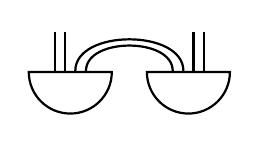
\begin{tikzpicture}[baseline, thick]
    \node[draw, shape=semicircle, shape border rotate=180, minimum size=1.5em] (x) at (0,0) {};
    \node[draw, shape=semicircle, shape border rotate=180, minimum size=1.5em] (y) at (1.5,0) {};
    \draw (x.130) -- +(0,0.5);
    \draw (x.105) -- +(0,0.5);
    \draw (x.75) to[out=90,in=90] (y.105);
    \draw (x.50) to[out=90,in=90] (y.130);
    \draw (y.75) -- +(0,0.5);
    \draw (y.50) -- +(0,0.5);
  \end{tikzpicture}
 \displaybreak[1] \\
(m_{4,6,2} : \V_4 \otimes \V_6 \to \V_6) & = 
  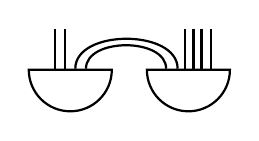
\begin{tikzpicture}[baseline, thick]
    \node[draw, shape=semicircle, shape border rotate=180, minimum size=1.5em] (x) at (0,0) {};
    \node[draw, shape=semicircle, shape border rotate=180, minimum size=1.5em] (y) at (1.5,0) {};
    \draw (x.130) -- +(0,0.5);
    \draw (x.105) -- +(0,0.5);
    \draw (x.75) to[out=90,in=90] (y.120);
    \draw (x.50) to[out=90,in=90] (y.140);
    \draw (y.100) -- +(0,0.5);
    \draw (y.75) -- +(0,0.5);
    \draw (y.55) -- +(0,0.5);
    \draw (y.40) -- +(0,0.5);
  \end{tikzpicture}
 \displaybreak[1] \\
\intertext{and}
(m_{4,4,1} : \V_4 \otimes \V_4 \to \V_6) & = 
  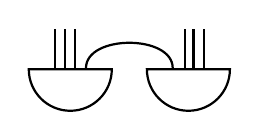
\begin{tikzpicture}[baseline, thick]
    \node[draw, shape=semicircle, shape border rotate=180, minimum size=1.5em] (x) at (0,0) {};
    \node[draw, shape=semicircle, shape border rotate=180, minimum size=1.5em] (y) at (1.5,0) {};
    \draw (x.130) -- +(0,0.5);
    \draw (x.105) -- +(0,0.5);
    \draw (x.75) -- +(0,0.5);
    \draw (x.50) to[out=90,in=90] (y.130);
    \draw (y.100) -- +(0,0.5);
    \draw (y.75) -- +(0,0.5);
    \draw (y.50) -- +(0,0.5);
  \end{tikzpicture}
\end{align*}
 as follows.

Recall that our chosen basis for $\V_4$ is
\[
  \left(
    \tikz[baseline=-7, thick]{\draw(0,0) arc (-180:0:0.2); \draw(0.6,0) arc(-180:0:0.2);},
    \tikz[baseline=-7, thick]{\draw(0,0) arc (-180:0:0.4); \draw(0.2,0) arc(-180:0:0.2);},
    \tikz[baseline=-7, thick]{\draw(0,0) arc (-180:0:0.2); \draw(0.6,0) arc(-180:0:0.2);
                       \draw(0.2,-0.2) arc (-180:0:0.3);},
    \tikz[baseline=-7, thick]{\draw(0,0) arc (-180:0:0.4); \draw(0.2,0) arc(-180:0:0.2);
                       \draw(0.4,-0.4) -- (0.4,-0.2);},
    \tikz[baseline=-7, thick]{\draw(0,0) arc (-180:0:0.3); \draw[knot] (0.3,0) arc (-180:0:0.3);}
  \right)
\]
Expressed in our chosen bases, we then have 
\begin{align*}
  m_{4,n,2}((x_1, x_2, x_3, x_4, x_5) \otimes y)
    & = x_1 \cup_{n-2}\cap_n y \\
      & \quad + x_2 y \\
      & \quad + x_3 \fork_{n-1}\fuse_n y \\
      & \quad + x_4 H_n y \\
      & \quad + x_5 \beta y.
\end{align*}
Finally, we can write $m_{4,4,1}$ in terms of the other operations, e.g.
as
$$
 m_{4,4,1}(x \otimes y) = m_{4,6,2}(x \otimes \rho_6^{-1} (\cup_4 (\rho_4(y)))
 = \begin{tikzpicture}[baseline, thick]
     \draw (0,0) arc (-180:0:0.5) -- cycle;
     \draw (2,0) arc (-180:0:0.5) -- cycle;
     \draw (2.2,0) arc (0:180:0.2) to[out=-90,in=180] (2.5,-0.65) to[out=0,in=-90] (3.2,0) arc (180:0:0.1) to[out=-90,in=0] (2.5,-0.8) to[out=180,in=-90] (1.2,0) arc (0:180:0.2);
     \draw (0.6,0) arc (180:0:0.4) arc (-180:0:0.1) -- +(0,0.4);
     \draw (0.2,0) -- +(0,0.4);
     \draw (0.4,0) -- +(0,0.4);
     \draw (2.4,0) -- +(0,0.4);
     \draw (2.6,0) -- +(0,0.4);
     \draw (2.8,0) -- +(0,0.4);
   \end{tikzpicture}
$$ 

\subsubsection{Conway width}
Typically, we may choose to think about a diagrammatically defined tangle
invariant as a morphism of planar algebras  $\mathsf{Tangle} \to \mathcal{Q}$
for some planar algebra $\mathcal{Q}$, sending the crossing to a suitable
element of $\mathcal{Q}_4$. In
our case we only know a limited set of operations in the target planar
algebra, and so can only compute the invariants of links which we can generate
from the crossing using those available planar operations.

\begin{definition}
The \emph{width} of a planar graph generically embedded in the plane is the 
maximum number of intersections with a horizontal line. The width of a planar
graph is the minimum width over all generic embeddings.

The \emph{Conway width} of a 4-valent planar graph is the width of the graph 
after repeatedly collapsing all digons. The Conway width of a link is the
Conway width of its shadow.
\end{definition}

It is easy to see that with the available planar operations, we can evaluate 
all Conway width 6 links.

\begin{lemma}
All knots and links with at most 12 crossings have Conway width at most 6, with exceptions of the two alternating links
$$
\diagram{0.2}{a6b1b1be704dda48723477a9c4e57cf27a610f7c} \qquad
\diagram{0.2}{d152a4e30d0711d71caa5a012365e5adbdcd5b2c}
$$
and their non-alternating cousins.
%% How did I generate these graphs?! I guess with DrawPlanarGraphApp.scala, setting `withOutputPath' appropriately?
% 12C = cuboctahedron
% a6b1b1be704dda48723477a9c4e57cf27a610f7c
% PlanarGraph(35,Vector(List(), List((5,6), (4,9), (3,8), (2,7)), List((2,6), (10,7), (9,18), (8,17)), List((8,6), (15,17), (14,27), (13,26)), List((10,18), (3,7), (19,8), (18,35)), List((18,18), (26,35), (25,46), (24,45)), List((24,18), (31,45), (15,27), (9,17)), List((26,46), (19,35), (35,8), (34,54)), List((34,46), (42,54), (41,65), (40,64)), List((40,46), (47,64), (31,27), (25,45)), List((42,65), (35,54), (4,8), (50,9)), List((50,65), (5,9), (13,6), (56,26)), List((56,65), (14,26), (47,27), (41,64))),Vector((2,0), (2,0), (2,0), (2,0), (2,0), (2,0), (2,0), (2,0), (2,0), (2,0), (2,0), (2,0)),0)
% 12G
% d152a4e30d0711d71caa5a012365e5adbdcd5b2c
% PlanarGraph(46,Vector(List(), List((5,6), (4,9), (3,8), (2,7)), List((2,6), (10,7), (9,18), (8,17)), List((8,6), (15,17), (14,27), (13,26)), List((13,6), (20,26), (19,36), (5,9)), List((26,36), (25,46), (24,45), (19,9)), List((20,36), (14,26), (30,27), (26,46)), List((10,18), (3,7), (34,8), (33,54)), List((4,8), (24,9), (40,45), (34,54)), List((25,45), (47,46), (46,75), (40,54)), List((54,75), (53,86), (33,18), (46,54)), List((15,27), (9,17), (53,18), (57,86)), List((47,75), (30,46), (57,27), (54,86))),Vector((2,0), (2,0), (2,0), (2,0), (2,0), (2,0), (2,0), (2,0), (2,0), (2,0), (2,0), (2,0)),0)
\end{lemma}
\begin{proof}
The Conway width of a link is the width of the Conway basic polyhedron 
obtained after collapsing all digons. One can enumerate the basic polyhedron
with $n$ vertices using Brinkmann and McKay's {\tt plantri} program
\cite{MR2357364,MR2186681}, with the command {\tt plantri -qda -c2 <n+2>}. 
All basic polyhedra with less than 12 vertices have width at most 6, and of 
the 12 vertex basic polyhedra all but 12C (the cuboctahedron) and 12G (using 
the naming scheme from \cite{MR679310}) have width at most 6. These graphs,
made into links, are the exceptions described above.
\end{proof}
In fact, almost all prime knots up to 11 crossings have bridge number 
at most 3, and hence width at most 6, with 15 exceptions, all Montesinos
knots.\footnote{The exceptions are 11a43, 11a44, 11a47, 11a57, 11a231,
  11a263, 11n71, 11n72, 11n73, 11n74, 11n75, 11n76, 11n77, 11n78, and
  11n81. \cite{1208.4233}}
Montesinos knots are easily seen to have Conway width 4.
Interestingly all knots with at most 14 crossings have Conway width at most 6.
If we were able to work with Conway width 8, we could nearly exhaust the 
available tables of knots and links; every Conway basic polyhedron with at 
most 19 vertices has width at most 8.

The obvious greedy algorithm (repeatedly collapse digons, when that is not
possible apply $m_{4,4,1}$ to merge two 4-boxes into a 6-box, and afterwards
hope that $m_{6,4,2}$  suffices to combine all remaining 4-boxes into that
6-box) works on all prime knots up to 12 crossings (for a handful of knots,
if you apply $m_{4,4,1}$ `in the wrong place' it is possible to get stuck ---
relabelling the strands and trying again quickly succeeds);
our tabulations described below are based on this algorithm.

\subsubsection{Examples}
Using the above observations, we have computed the (conjectural!) 
invariant $\xi$ of all prime links up to 11 crossings, and all prime knots up
to 12 crossings. We observe that these values of $\xi$ are always of the form
$$\xi(L) - d^{k} = 
\frac{[4][6][\lambda-6][\lambda+5]}{[2][\lambda]^k [\lambda-1]^k} \mathcal E(L),$$
where 
$$d = \xi(\textrm{unknot}) = 
-\frac{\left(v^2+v^{-2}\right) \left(\frac{w}{v^6}-\frac{v^6}{w}\right) \left(v^5 w-v^{-5} w^{-1}\right)}{\left(w-w^{-1}\right)
   \left(\frac{w}{v}-\frac{v}{w}\right)},$$ $k$ is the number of components of $L$, 
and $\mathcal E(L)$ is some Laurent polynomial
in $v$ and $w$. We offer no explanation at this point for this factorisation behaviour.
These polynomials $\mathcal E (L)$ are tabulated
at \url{https://tqft.net/papers/QES-Knot-Polynomials.m.gz} and in the ancillary files
with the {\tt arXiv} version of this paper.

It would be desirable to verify directly that these computed invariants specialize 
correctly to the quantum link invariants of the adjoint representations of the
exceptional Lie algebras. (Of course, we have proved unconditionally \nn{where?}
that these do in fact
specialize correctly --- but it would be nice to be able to check computations.)
Unfortunately, these invariants have previously been
rather hard to compute, so there is little available to check against. The Lie
algebra $\mathfrak{sl}_2$ lies on the exceptional curve, and so the 2nd
coloured Jones polynomial  (that is, colored by the 3-dimensional adjoint
representation) should be the $v=q^{1/3}$, $w=\pm q^{4/3}$ or $w=\pm q^{-1}$ specialisation. This is
indeed the case for all the prime links up to 9 crossings, and all the prime knots up to 10 crossings. \nn{check further?}

Even for the adjoint representation of $G_2$, an earlier program by the first
author for computing quantum knot invariants gets only as far as the trefoil. 
Sure enough, we have
\begin{align*}
\xi(3_1) & = 
-\frac{v^{12} \left(v^4+1\right) \left(v^{12}-w^2\right) \left(v^{10} w^2-1\right)}{w^4 \left(w^2-1\right) \left(w^2-v^2\right)} \times \\
& \quad \times
\big(v^{36} w^4-v^{36} w^2-v^{34} w^6+v^{34} w^4-v^{32} w^4+v^{32} w^2+v^{30} w^6+v^{28} w^4-v^{28} w^2-v^{26} w^6 \\
& \qquad +v^{26} w^2-v^{26}+v^{24} w^6-3 v^{24} w^4+v^{24} w^2-v^{22} w^8+v^{22} w^6-v^{22} w^4-v^{22} w^2-v^{20} w^6 \\
& \qquad +2 v^{20} w^4-v^{20} w^2-v^{18} w^6+v^{18} w^2+v^{16} w^6-v^{16} w^4+v^{16} w^2+v^{16}+v^{14} w^6+v^{14} w^4 \\
& \qquad -v^{14} w^2+v^{14}+v^{12} w^8-v^{12} w^6+2 v^{12} w^4+v^{10} w^8+v^{10} w^2+v^8 w^6-v^8 w^4-v^6 w^2 \\
& \qquad -v^4 w^6-v^4  -v^2 w^4-w^8-w^4\big)
\intertext{which at $v= q^2, w= q^5$ gives}
& = q^{144}-q^{126}+q^{122}-q^{116}+2 q^{112}+q^{110}-q^{108}+2 q^{104}+q^{102}-q^{98}-q^{96}+q^{94}-2 q^{90}-2 q^{88} \\ 
& \qquad -q^{86}-q^{84}-2 q^{82}-3 q^{80}-2 q^{78}-2 q^{76}-
  2 q^{74}-2 q^{72}-2 q^{70}-q^{68}-q^{64}-q^{62}+q^{60}+q^{58} \\
& \qquad +q^{56}+2 q^{54}+q^{52}+2 q^{50}+3 q^{48}+2 q^{46}+
   2 q^{44}+3 q^{42}+2 q^{40}+2 q^{38}+3 q^{36}+2q^{34}+q^{32} \\
& \qquad +2 q^{30}+q^{28}+q^{26}+q^{24}+q^{18},
\end{align*}
agreeing with the direct calculation using $R$-matrices.
One could also attempt to use the adjoint representation skein theory for $G_2$ from
\cite{MR1403861}, although we haven't pursued this.

As an example,
the value of $\xi(8_{18})$, the first non-algebraic knot, is too large to display here. (It has 426 monomial terms.)
Its specialisation to the quantum $E_8$ curve shows that the $E_8$ adjoint quantum knot invariant is
\begin{multline*}
\frac{\left(q^4+1\right)^2 \left(q^{16}-q^{12}+q^8-q^4+1\right)}{q^{306}} 
   \times \\ \displaybreak[2]
\quad \times
\Big(
q^{92}+q^{90}+q^{84}+q^{82}+q^{80}+q^{78}+q^{76}+q^{74}+q^{72}+q^{70}+2 q^{68}+2q^{66}+q^{64}+q^{62}+2 q^{60}+2 q^{58} \\\qquad
+2 q^{56}+2 q^{54}+2 q^{52}+2 q^{50}+2 q^{48}+2 q^{46}+2 q^{44}+2 q^{42}+2 q^{40}+2 q^{38}+2 q^{36}+2 q^{34}+2q^{32} \\\qquad
+q^{30}+q^{28}+2 q^{26}+2 q^{24}+q^{22}+q^{20}+q^{18}+q^{16}+q^{14}+q^{12}+q^{10}+q^8+q^2+1\Big) \times \\ \displaybreak[1]
\quad \times 
\Big(
q^{496}-4 q^{494}+6 q^{492}-4 q^{490}+q^{488}-4q^{484}+16 q^{482}-24 q^{480}+16 q^{478}-8 q^{476}+16 q^{474}-18 q^{472} \\\qquad
-8 q^{470}+32 q^{468}-24 q^{466}+18 q^{464}-52 q^{462}+80 q^{460}-44 q^{458}+2 q^{456}-24q^{454}+44 q^{452}+20 q^{450} \\\qquad
-93 q^{448}+64 q^{446}-18 q^{444}+92 q^{442}-183 q^{440}+116 q^{438}-12 q^{436}+85 q^{434}-193 q^{432}+67 q^{430} \\\displaybreak[2]\qquad
+153 q^{428}-132q^{426}+20 q^{424}-211 q^{422}+517 q^{420}-433 q^{418}+126 q^{416}-191 q^{414}+461 q^{412}-237 q^{410} \\\qquad
-333 q^{408}+409 q^{406}-85 q^{404}+302 q^{402}-959 q^{400}+946q^{398}-274 q^{396}+215 q^{394}-823 q^{392}+678 q^{390} \\\qquad
+360 q^{388}-685 q^{386}-89 q^{382}+1327 q^{380}-1728 q^{378}+681 q^{376}-368 q^{374}+1555 q^{372}-1822q^{370} \\\qquad
+143 q^{368}+927 q^{366}+14 q^{364}-256 q^{362}-1762 q^{360}+3103 q^{358}-1709 q^{356}+575 q^{354}-2107 q^{352} \\\displaybreak[2]\qquad
+3153 q^{350}-948 q^{348}-1332 q^{346}+320q^{344}+836 q^{342}+1501 q^{340}-4105 q^{338}+2762 q^{336}-556 q^{334} \\\qquad
+2184 q^{332}-4575 q^{330}+2573 q^{328}+973 q^{326}-291 q^{324}-1979 q^{322}-276 q^{320}+4567q^{318}-4155 q^{316} \\\qquad
+1041 q^{314}-2351 q^{312}+6237 q^{310}-5072 q^{308}+117 q^{306}+459 q^{304}+2619 q^{302}-1072 q^{300}-4676 q^{298} \\\qquad
+5789 q^{296}-1865 q^{294}+1886q^{292}-6637 q^{290}+6941 q^{288}-1317 q^{286}-768 q^{284}-2887 q^{282}+2954 q^{280} \\\displaybreak[2]\qquad
+3203 q^{278}-6066 q^{276}+2166 q^{274}-890 q^{272}+6141 q^{270}-8532 q^{268}+3377q^{266}+87 q^{264}+3441 q^{262} \\\qquad
-5066 q^{260}-965 q^{258}+5826 q^{256}-2922 q^{254}+494 q^{252}-5390 q^{250}+9551 q^{248}-5390 q^{246}+494 q^{244} \\\qquad
-2922 q^{242}+5826q^{240}-965 q^{238}-5066 q^{236}+3441 q^{234}+87 q^{232}+3377 q^{230}-8532 q^{228}+6141 q^{226} \\\displaybreak[2]\qquad
-890 q^{224}+2166 q^{222}-6066 q^{220}+3203 q^{218}+2954 q^{216}-2887q^{214}-768 q^{212}-1317 q^{210}+6941 q^{208} \\\qquad
-6637 q^{206}+1886 q^{204}-1865 q^{202}+5789 q^{200}-4676 q^{198}-1072 q^{196}+2619 q^{194}+459 q^{192}+117 q^{190} \\\qquad
-5072q^{188}+6237 q^{186}-2351 q^{184}+1041 q^{182}-4155 q^{180}+4567 q^{178}-276 q^{176}-1979 q^{174}-291 q^{172} \\\qquad
+973 q^{170}+2573 q^{168}-4575 q^{166}+2184 q^{164}-556q^{162}+2762 q^{160}-4105 q^{158}+1501 q^{156}+836 q^{154} \\\displaybreak[2]\qquad
+320 q^{152}-1332 q^{150}-948 q^{148}+3153 q^{146}-2107 q^{144}+575 q^{142}-1709 q^{140}+3103 q^{138}-1762q^{136} \\\qquad
-256 q^{134}+14 q^{132}+927 q^{130}+143 q^{128}-1822 q^{126}+1555 q^{124}-368 q^{122}+681 q^{120}-1728 q^{118} \\\qquad
+1327 q^{116}-89 q^{114}-685 q^{110}+360q^{108}+678 q^{106}-823 q^{104}+215 q^{102}-274 q^{100}+946 q^{98}-959 q^{96} \\\qquad
+302 q^{94}-85 q^{92}+409 q^{90}-333 q^{88}-237 q^{86}+461 q^{84}-191 q^{82}+126q^{80}-433 q^{78}+517 q^{76}-211 q^{74} \\\qquad
+20 q^{72}-132 q^{70}+153 q^{68}+67 q^{66}-193 q^{64}+85 q^{62}-12 q^{60}+116 q^{58}-183 q^{56}+92 q^{54}-18 q^{52} \\\qquad
+64 q^{50}-93q^{48}+20 q^{46}+44 q^{44}-24 q^{42}+2 q^{40}-44 q^{38}+80 q^{36}-52 q^{34}+18 q^{32}-24 q^{30}+32 q^{28} \\\qquad
-8 q^{26}-18 q^{24}+16 q^{22}-8 q^{20}+16 q^{18}-24 q^{16}+16q^{14}-4 q^{12}+q^8-4 q^6+6 q^4-4 q^2+1\Big)
\end{multline*}
which was previously far from accessible. \nn{I'm very happy to remove this ridiculuous waste of space, but
thought I would try including an explicit example for flavour.}
 
We can evaluate a variety of knotted trivalent graphs, although the actual values are mostly too complicated
to warrant repeating here.
\begin{align*}
\xi\left(\mathfig{0.05}{knotted-theta}\right) & = 
\frac{\left(v^4+1\right) \left(v^6-w\right) \left(v^6+w\right) \left(v^5 w-1\right)\left(v^5 w+1\right) }{v^{36} (w-1) w^4 (w+1) (v-w) (v+w)} \times \\
& \quad \times
\big(v^{30} w^4-v^{30} w^2+v^{30}-v^{28} w^6+v^{28} w^4+v^{26} w^8-v^{26} w^4+v^{26} w^2+v^{24} w^6+v^{24} w^4 
   \\ 
& \qquad -2 v^{24} w^2+v^{24}-2 v^{22} w^6+3 v^{22} w^4-v^{22} w^2+v^{20} w^8-v^{20} w^6-2 v^{20} w^4+2 v^{20} w^2 \\
& \qquad -v^{20} +2 v^{18} w^6-2 v^{18} w^4-v^{16} w^8+3 v^{16} w^4-2 v^{16} w^2-2 v^{14} w^6+2 v^{14} w^2-v^{14} \\
& \qquad +2 v^{12} w^6-5 v^{12} w^4 +2 v^{12} w^2-v^{10} w^8+2 v^{10} w^6-v^{10}
   w^2-v^8 w^6+2 v^8 w^4-v^6 w^4 \\
& \qquad +v^6 w^2+v^4 w^6-v^4 w^4+v^2 w^4-v^2 w^2-w^6+w^4\big)
\end{align*}
Each of the random selections from the list of 7-crossing knotted thetas
\cite{MR2507922} we tried is computable. We can also compute the value of the
dodecahedron --- even though we haven't explicitly written down
any relation that reduces the docadecahedron, one can easily check it has girth 6, and
can be written in terms of the planar operations discussed above.

\subsubsection{Comparisons}

Some previous work has calculated universal knot invariants, which can be
thought of as the knot invariants coming from the putative quantized Vogel
plane (and hence these have specializations to the quantum knot invariants of
any adjoint representation, exceptional or not). Mironov--Mkrtchyan--Morozov
\cite{MR3491191} explains the calculation of the universal knot invariants for
all 2- and 3-strand torus knots. Westbury \cite{1510.08307} explains the
context of the quantized Vogel plane, and gives the invariants for $(2,n)$
torus knots, in \S 6.1. Finally Mironov--Morozov \cite{MR3475991} explains how
to calculate the universal invariants for all algebraic (or arborescent) links. (Note that
the class we calculate above includes many non-algebraic links. The first is
$8_{18}$.)


\section{Special values}
\label{sec:special-values}

\DPTtodo{Made this section more general, since it seems other special cases
  naturally go here}
The goal of this section is to analyze several special cases,
including
\begin{itemize}
\item When $v$ is a $10$th or $12$th root of unity, the
  derivation of the QESquare and QECrossing relations break down.
\item When $\fg$ is in Deligne's list, in the adjoint
  representation, the conjectural 2-variable polynomial specializes
  correctly.
\item The $7$-dimensional representation of $U_q(\fg_2)$ also
  satisfies the given assumptions on the dimension of the 4-box space.
\item For $U_q(\fg)$ for $\fg$ in the $F_4$ family, we again have a
  trivalent vertex. At $q=1$ we have $v^6 = -1$, since the trivalent
  vertex is symmetric, not anti-symmetric. This family has only a
  finite number of points.
  \DPTtodo{Also classical $S_t$?}
\end{itemize}

Here's a rough sketch of the proof given in Section \ref{sec:special-values}.
(Some modification is
needed for $\mathrm{OSp}(1|2)$.)  All the skein relations in
$\mathsf{Exc}_{\mathbb{C},\lambda}$ do hold in the corresponding
representation categories, so we get a functor which is injective on morphisms
and essentially surjective on objects.  By Tannaka--Krein duality and
unitarity, the image of this functor is the category of representations of a
subgroup of the orthogonal group $\mathrm{O}(\mathfrak{g})$ preserving the bracket and containing
the group.  But each of these groups is the maximal such unitary group
preserving the bracket, so the functor is surjective on morphisms.


\subsection{Specialisations to exceptional Lie algebras}%

We begin by proving classical specialization.  This argument is essentially the same as the one in \nn{Etingof-Neshveyev}

\begin{proposition}[Classical specialization]
If Conjecture \ref{conj:class-suffic} holds and $\lambda$ is one of
the values on the left of Table~\ref{tab:lambda-group}, then the
idempotent completion of the quotient of
$\mathsf{Exc}_{\mathbb{C},\lambda}$ by negligible elements is equivalent
to the category of representations of the corresponding group on the
right of Table~\ref{tab:lambda-group}.
\end{proposition}
\begin{proof}
Let $G$ be one of the compact groups in the table and $\lambda$ the corresponding special value.
$\mathrm{Rep}(G)$ is a symmetric monoidal category and the Killing form shows that the adjoint representation is symmetrically self-dual.   
Since $\mathfrak{g}$ is a Lie algebra, we have a bracket map of $G$-reps $\mathfrak{g} \otimes \mathfrak{g} \rightarrow \mathfrak{g}$.  Hence we have a monoidal functor from the TriCat \nn{notation} to $\mathrm{Rep}(G)$ sending the strand to the adjoint representation and the trivalent vertex to the bracket. Since $\mathfrak{g}$ is a Lie algebra, the Jacobi and anti-symmetry relations hold.  By results of \nn{add citations} the classical exceptional relation with parameter $\lambda$ holds.  Hence the functor descends to one out of $\mathsf{Exc}_{\mathbb{C},\lambda}$.  %By Conjecture \ref{conj:class-suffic} we have that the unit object in $\mathsf{Exc}_{\mathbb{C},\lambda}$ is simple. 
By postcomposing with the fiber functor for $\mathrm{Rep}(G)$, we see that $\mathsf{Exc}_{\mathbb{C},\lambda}$ has a fiber functor to vector spaces.  By Tannaka-Krein duality, we see that 
\end{proof}








 

\begin{center}
\begin{tabular}{llll}
 & $v$ & $w$ & $V$ \\
\midrule
\midrule
$E_8$              & $q^5$              & $\pm q^6$ or $\pm q^{-1}$                & $V_{e_8}$       \\
$E_7$              & $q^3$              & $\pm q^4$ or $\pm q^{-1}$                & $V_{e_1}$       \\
$E_6^{\bbZ/2\bbZ}$ & $q^2$              & $\pm q^3$ or $\pm q^{-1}$                & $V_{e_2}$       \\
$F_4$              & $q^3$              & $\pm q^5$ or $\pm q^{-2}$                & $V_{(1,0,0,0)}$ \\
$D_4^{S_3}$        & $q  $              & $\pm q^2$ or $\pm q^{-1}$                & $V_{(0,1,0,0)}$ \\
$G_2$              & $q^2$              & $\pm q^5$ or $\pm q^{-3}$                & $V_{(0,1)}$     \\
$A_2^{\bbZ/2\bbZ}$ & $q^{1/2}$          & $\pm q^{3/2}$ or $\pm q^{-1}$            & $V_{(1,1)}$     \\
$A_1$              & $q^{1/3}$          & $\pm q^{4/3}$ or $\pm q^{-1}$            & $V_{(2)}$       \\
\midrule
$F_4$              & $\pm i q^2$        & $\pm i q^3$ or $\pm q^{-1}$              & $V_{(0,0,0,1)}$ \\
$C_3$              & $\pm i q$          & $\pm i q^2$ or $\pm q^{-1}$              & $V_{(0,1,0)}$   \\
$A_2^{\bbZ/2\bbZ}$ & $\pm i q^{1/2}$    & $\pm i q^{3/2}$ or $\pm q^{-1}$          & $V_{(1,1)}$     \\
$A_1$              & $\pm i q$          & $\pm i q^5$ or $\pm q^{-4}$              & $V_{(4)}$       \\
\midrule
$G_2$              & $\zeta_3^{\pm1} q$ & $\pm \zeta_3^{\pm1} q^2$ or $\pm q^{-1}$ & $V_{(1,0)}$     \\
$A_1$              & $\zeta_3^{\pm1} q$ & $\pm \zeta_3^{\pm1} q^4$ or $\pm q^{-3}$ & $V_{(2)}$       \\
\bottomrule
\end{tabular}
\end{center}
(Signs are independent, except on the last two rows where one needs to use the same choice in $\zeta_3^{\pm1}$ for both $v$ and $w$.)

We can find the intersections of these subvarieties. If the quantum sufficiency conjecture holds, we would deduce the  braided equivalences below. Each triple $((\Gamma)_k,V,q)$ indicates the (semisimplified) quantum group representation  category for the Lie algebra $\Gamma$, tensored generated by the irreducible $V$, at the root of unity $q$. The subscript $k$ indicates the level, but this does not completely specify the (braided) category, which depends on the value of $q$ --- although of course all such categories are Galois conjugates. The parameter $q$ is written using the shorthand $\zeta_n = \exp(2 \pi i/n)$. Each equivalence takes the tensor generator to the tensor generator.
\begin{align*}
((A_1)_7,V_{(4)},\zeta_{18}) & \cong ((G_2)_2,V_{(1,0)},\zeta_{36}^{35}) &
((A_1)_{12},V_{(4)},\zeta_{14}) & \cong ((A_2^{\bbZ/2\bbZ})_4,V_{(1,1)},\zeta_{28}^9) \\
((A_1)_3,V_{(2)},\zeta^{10}) & \cong ((G_2)_1,V_{(1,0)},\zeta_{30}^{13}) &
((A_1)_6,V_{(2)},\zeta_{16}) & \cong ((A_1)_6,V_{(4)},\zeta_{16}^5) \\
((A_1)_9,V_{(4)},\zeta_{22}) & \cong ((F_4)_2,V_{(0,0,0,1)},\zeta_{44}) &
((A_1)_{10},V_{(4)},\zeta_{24}) & \cong ((C_3)_2,V_{(0,1,0)},\zeta_{24}) \\
((C_3)_{1/2},V_{(0,1,0)},\zeta_{18}) & \cong ((G_2)_{2},V_{(1,0)},\zeta_{36}^5) &
((E_7)_{3},V_{e_1},\zeta_{42}) & \cong ((G_2)_3,V_{(1,0)},\zeta_{42}^{17}) \\
((F_4)_{1/2},V_{(1,0,0,0)},\zeta_{19}) & \cong ((G_2)_{7/3},V_{(0,1)},\zeta_{38}^3) &
((F_4)_{3},V_{(0,0,0,1)},\zeta_{48}) & \cong ((G_2)_4,V_{(1,0)},\zeta_{48}^{19}) \\
((F_4)_{4},V_{(1,0,0,0)},\zeta_{52}) & \cong ((F_4)_4,V_{(0,0,0,1)},\zeta_{52}^{21}) &
((G_2)_{1/3},V_{(0,1)},\zeta_{26}) & \cong ((A_1)_{24},V_{(4)},\zeta_{52}^{17}) \\
((G_2)_{2/3},V_{(0,1)},\zeta_{28}) & \cong ((C_3)_{3},V_{(0,1,0)},\zeta_{28}^9) &
((G_2)_{3},V_{(0,1)},\zeta_{21}) & \cong ((G_2)_3,V_{(1,0)},\zeta_{21}^{16}) \\
\end{align*}


\hrule

We begin by analyzing what happens when $\dim \cC_4 < 5.$


\subsection{Quantum exceptional relation for special cases}

In this section we collect the values of $v$ and $\alpha$ for which each known example satisfies the QEJacobi relation.  

\begin{equation*}
\left[\; v^{-3} \;
\drawcrossX
\;+ v \;
\drawI
\; -v^{-1} \;
 \drawH
\;\right]
 + \alpha
\left[\; \braidcross \;
 + v^{4}\;
\cupcap
\; + v^{-4} \;
 \twostrandid \;
 \right] = 0.
 \end{equation*}
 
Recall that there's a symmetry $(v,\alpha) \mapsto (-v,-\alpha)$ where they give the same relation, and we only record one version of each relation.

We will also say that the QEJacobi relation holds with $\alpha=\infty$ if

\begin{equation*}
\braidcross \;
 + v^{4}\;
\cupcap
\; + v^{-4} \;
 \twostrandid \;= 0.
 \end{equation*}

Each of the following lemmas is proved the same way.  We compute the value of the trivalent twist which gives the value of $-v^6$.  This leaves three options (up to sign) for $v$.  Then we take a relation $X$ between the six diagrams and compute $X+v^{4} R(X)+ v^{-4}R^2(X)$ to get QEJacobi relations. 

\begin{lemma}
$SO(3)_q$ satisfies three instances of the QEJacobi relation with $\alpha = -b \frac{\Psi_1(v)}{\Psi_{12}(v)} $ for $v$ a cube root of $q$.  Under the change of variables we see that this value of $\alpha$ corresponds to $w = \pm v^4$ or $w = \pm v^{-3}$.
\end{lemma}

\begin{lemma}
The golden categories are quotients of $SO(3)_q$ at $q$ a fifth or tenth root of unity.  In addition to the three relations in the previous lemma there's an additional relation $\alpha=\infty$ and $v = q^{\frac{1}{2}}$ (any choice square root gives the same relation).
%I don't think these are quite right
% \begin{itemize}
% \item $\alpha=\infty$ and $v = e^{\frac{2 \pi i}{5}}$
%  \item $\alpha = b\left(1-\frac{v^{-3}}{v^{12}-v^{-12}}\right)$ and $v = e^{\frac{2 \pi i}{5}}$
% \item $\alpha = b\left(1-\frac{v^{-3}}{v^{12}-v^{-12}}\right)$ and $v = e^{3 \frac{2 \pi i}{10}}$
% \item $\alpha = b\left(1-\frac{v^{-3}}{v^{12}-v^{-12}}\right)$ and $v = e^{7 \frac{2 \pi i}{10}}$ 
%\end{itemize}
 \end{lemma}
 \begin{proof}
Plug the golden category formula for the $I$-diagram into the $SO(3)_q$ braiding relation to get a formula for the crossing in terms of the Temperley-Lieb diagrams.
 \end{proof}

\begin{lemma}
$(G_2)_q$ satisfies two instances of the QEJacobi relation, $\alpha = b \frac{1-\zeta q^2}{-\zeta^2 q}$ and $v = \zeta q$ for $\zeta$ a primitive cube root of unity.  This value of $\alpha$ corresponds to $w = \pm q^{-1} = \pm \zeta v^{-1}$ or $w = \pm \zeta q^2 = \pm \zeta^2 v^2$.
\end{lemma}

\begin{lemma}
$S_{d+1}$ satisfies two instances of the QEJacobi relation $\alpha = -v^3 \frac{b}{d-1}$ for $v$ a primitive $12$th root of unity.
\end{lemma}

\begin{lemma}
$\Rep(S_3)$ satisfies three instances of the QEJacobi relation
\begin{itemize}
\item $v = e^{\frac{2 \pi i}{12}}$ and $\alpha = -i b$
\item $v = e^{\frac{-2 \pi i}{12}}$ and $\alpha = i b$
\item $v = i$ and $\alpha = -\frac{i}{2} b$.
\end{itemize}
\end{lemma}











\subsection{Corner cases with small 4-box space}

\begin{lemma}
The diagrams
$$\cupcap \text{ and } \twostrandid$$
are non-zero and are linearly independent.
\end{lemma}
\begin{proof}
If either diagram is zero then by multiplying by a crossing on the appropriate side you get that the trivalent vertex is zero, which is a contradiction.  If the two diagrams are linearly dependent, then again multiplying by a trivalent vertex would show that the trivalent vertex is zero.
\end{proof}


\nn{Move the following to the background section}
The following lemma is a mild generalization of \nn{Noah: what did you intend to cite here? \cite[Theorem 3.4]{MR3449240}?} where we have relaxed the non-degeneracy assumption.


\begin{lemma}
Suppose that the diagrams   
  \[
  \cupcap\;,\qquad\twostrandid\;,
    \qquad\drawI\;,\qquad\drawH\;\;
   \]
are linearly dependent, then
 
$$\drawI\; - \; \drawH - \frac{1}{d-1} \left(\; \twostrandid - \cupcap \; \right) = 0.$$
\end{lemma}
\begin{proof}
By the previous lemma, we must have a relation of the form:
$$\drawI\;\pm \; \drawH = z \left(\; \twostrandid \pm \cupcap \;\right).$$

Capping off we see that $b= z (d \pm 1)$, so $z = \frac{b}{d \pm 1}$.  So all we need to do is exclude the $+$-sign case.

Attaching a trivalent vertex we see that $t + b = \frac{b}{d + 1}$, so $t =  -\frac{b d}{d + 1}$.  Adding $\drawH$ to the top gives:

$$t \drawI + \fourgon = \frac{b}{d+1} \left(\; \drawH + b \cupcap \; \right).$$

If we take this relation minus its $90$-degree rotation the square term will vanish yielding:
$$ b \frac{d-1}{d+1} \left(\; \drawI -\drawH \; \right) = \frac{b^2}{d+1} \left(\; \twostrandid - \cupcap \; \right).$$
Dividing by $b \frac{d-1}{d+1}$ yields the desired equation.
\end{proof}

By Lemma \ref{lem:IequalsH} we have the following Corollary.

\begin{corollary}
If the diagrams   
  \[
  \cupcap\;,\qquad\twostrandid\;,
    \qquad\drawI\;,\qquad\drawH\;\;
   \]
are linearly dependent, then
\begin{itemize}
\item $v$ is a primitive $12$th root of unity
\item $\cC$ is a quotient of $SO(3)_q$ with the usual braiding
\item $\cC$ is $\mathsf{Rep}(S_3)$ with its symmetric braiding.
\end{itemize}
\end{corollary}


\begin{proposition} \label{prop:dim4}
If the diagrams  
  \[
  \cupcap\;,\qquad\twostrandid\;,
    \qquad\drawI\;,\qquad\drawH\;,\qquad\braidcross\;,\qquad\fourgon\;
   \]
span a space of dimension $4$ or smaller, then
\begin{itemize}
\item $v$ is a primitive $12$th root of unity
\item $\cC$ is a quotient of $SO(3)_q$ with the usual braiding.
\item $\cC$ is $\mathsf{Rep}(S_3)$ with its symmetric braiding.
\item $\cC$ is a quotient of $(G_2)_q$ with the usual braiding.  \NStodo{Which QEJacobi hold?}
\end{itemize}
\end{proposition}
\begin{proof}
If the first four diagrams are linearly dependent then we're in one of the
first three cases.  Otherwise, we have a relation simplifying both the
crossing and the square in terms of the first four diagrams.  This means that
$\cC$ is generated by the trivalent vertex and $\dim \cC_4 \leq 4$, and thus
by a modification, explained in the next remark, of \cite[\S 5]{MR3624901} we see that $\cC$ is a
quotient of $(G_2)_q$.
\end{proof}

\begin{remark}
Strictly speaking in \cite{MR3624901} we only considered non-degenerate trivalent categories, but this can be avoided as follows.  The argument that the pentagon reduces still applies, so all small faces reduce, and non-elliptic diagrams span all $\cC_k$.  If the $10$ non-elliptic diagrams in $\cC_5$ are independent then Kuperberg \cite{MR1265145} says that $\cC$ is a quotient of $(G_2)_q$.  If there's a relation between these ten diagrams, the relation must be negligible.  By \cite{MR3624901} either there's a single relation and the category is a quotient of $(G_2)_{\zeta_{10}}$, or the non-degenerate quotient of $\cC$ is an $ABA$ category which contradicts $\cC$ being braided.
\end{remark}



\subsection{The case \texorpdfstring{$v = \pm 1$}{v = pm 1}}

Throughout this section we assume $v=1$.

Recall $t = \frac{b-[5]\alpha}{\{2\}} = \frac{b}{2}$.  We also have that $0= [5]b = -\alpha (d+\{8\})$, so we split into two cases based on whether $\alpha = 0$.

\begin{lemma}
There are no $\cC$ with $\alpha \neq 0$.
\end{lemma}
\begin{proof}
Since $d+\{8\}=0$, we have that $d=-2$.  The QECrossing relation says that:
$$\braidcross + \cupcap + \twostrandid = 0.$$
This is exactly the case excluded in Lemma \ref{lem:betazero}.
\end{proof}

\begin{lemma}
If $\alpha = 0$, then $\cC$ satisfies the defining relations of the classical exceptional series.
\end{lemma}
\begin{proof}
QECrossing says that the crossing is symmetric, and then QEJacobi becomes the usual Jacobi relation. 

Since $\dim \cC_4 \leq 5$, there must be some relation of the following form:
$$0 = \fourgon + x \symcross + y \left(\drawI + \drawH \right) + z\left(\twostrandid + \cupcap \right).$$
Multiplying this by a crossing and using the Jacobi relation:
\begin{align*}
0 &= \fourgon - \frac{b}{2} \drawI + x \twostrandid + y \left(-\drawI + \drawH -\drawI \right) + z\left(\symcross + \cupcap \right) 
\\ &= \fourgon + z \symcross + \left(-2y -\frac{b}{2} \right) \drawI +y \drawH +x \twostrandid + z\cupcap. 
\end{align*}

If these two relations are distinct, then Proposition \ref{prop:dim4} applies, and the only case with $v=1$ is classical $SO(3)$ (note that there is not trivalent category $(G_2)_{\zeta_3}$), which satisfies the classical exceptional relation.  Otherwise, we have $x=z$ and $y = -\frac{b}{6}$.  

Capping off this relation gives $0 = b^2 + x -\frac{b^2}{6}+x(1+d) =  (2+d)x +\frac{5 b^2}{6}$, so we have $x = -\frac{5 b^2}{6(2+d)}$.  This gives the classical exceptional square relation.
\end{proof}


\subsection{The case \texorpdfstring{$v$}{v} is a primitive third or sixth root of unity}

\begin{proposition}
If $v$ is a primitive third root of unity, then $\cC$ is classical $SO(3)$ or classical $G_2$.
\end{proposition}
\begin{proof}
Since $v$ is not a $10$th root of unity $\alpha$ is non-zero.  Also $b+[3]\alpha = b \neq 0$.  QECrossing says that the braiding is symmetric.  
%QEJacobi becomes $$\drawsymcrossX + v \drawI - v^2 \drawH + \alpha \left(\symcross + v^2 \twostrandid +v \cupcap \right) = 0.$$

QESquare becomes:
$$\symcross+\frac{\sqrt{-3}}{2\alpha} \left(\drawI + \drawH \right) -\frac{1}{2} \left(\twostrandid + \cupcap \right) = 0.$$

After rescaling the trivalent vertex, this becomes precisely the Hurwitz relation (or classical $G_2$ relation) of \cite{1011.6197}.  The main result of that paper is that either $d = 7$ and $\cC$ is classical $G_2$ or $d=3$ and $\cC$ is $SO(3)$.
\end{proof}

\subsection{The case \texorpdfstring{$v$}{v} is a primitive fourth root of unity}

Since $v$ is not a $10$th root of unity $\alpha$ is nonzero.  We have that $d+2 = \frac{-2ib}{\alpha}$.
We need to split into two cases based on whether $b+[3]\alpha = 0$.  

\begin{proposition}
If $b+[3]\alpha \neq 0$ then $\cC$ satisfies the relations of the classical F4 relation.  In particular the non-degenerate quotient of $\cC$ must be one of \nn{LIST}.
\end{proposition}
\begin{proof}
If $b+[3]\alpha \neq 0$, then QECrossing says the crossing is symmetric.   QEJacobi becomes
$$\drawsymcrossX + \drawI + \drawH = \alpha i \left(\symcross + \twostrandid + \cupcap \right).$$  If we rescale the trivalent vertex so that $\alpha i = 2$ then $b = d+2$ we have exactly the classical F4 relation.  The main result of \cite{F4E6} is that this forces one of the following possibilities:

\nn{TABLE}

We exclude the $\Rep(S_3)$ case because it satisfies $b+[3]\alpha = 0$.
\end{proof}

Since we do not know whether the classical F4 relation is sufficient for evaluating all closed diagrams, we do not know whether there are any additional degenerate $\cC$ whose non-degenerate quotient is one of the above categories.

If $b+[3]\alpha = 0$, then $\alpha = -\frac{bi}{2}$ and $d = 2$.  QEJacobi becomes
$$\drawcrossX + \drawI + \drawH = \frac{1}{2} \left(\braidcross + \twostrandid + \cupcap \;\right).$$
QESquare becomes
$$\fourgon = -\frac{1}{2} \left(\drawI + \drawH \;\right) + \frac{1}{2} \left(\;\twostrandid + \cupcap \;\right).$$

\begin{lemma}
The following diagrams are negligible in $\cC$:
\begin{itemize}
\item $$\braidcross + \invbraidcross - 2 \left(\drawI + \drawH \;\right)$$
\item $$\braidcross - \invbraidcross$$
\item $$\left(\drawI - \drawH - \twostrandid + \cupcap\;\right).$$
\end{itemize}
\end{lemma}
\begin{proof}
If the diagrams
  \[
  \cupcap\;,\qquad\twostrandid\;,
    \qquad\drawI\;,\qquad\drawH\;,\qquad\braidcross\;,\qquad\fourgon\;
   \]
 span a $4$-dimensional space then the first $4$ diagrams span by Proposition \ref{prop:dim4}\NStodo{Add this statement to Prop \ref{prop:dim4}}.  If these $5$ diagrams are linearly independent then since $\dim \cC_4 \leq 5$, then they span.  Thus in either case we can check whether an element is negligible by pairing it with the above $5$ diagrams.
\end{proof}

\begin{corollary}
If $\cC$ is non-degenerate then it must be $\mathsf{Rep}(S_3)$.
\end{corollary}

\begin{corollary}
Either
\begin{itemize}
\item $$\braidcross + \invbraidcross = 2 \left(\drawI + \drawH \;\right).$$
\item $$\braidcross - \invbraidcross = x \left(\drawI - \drawH - \twostrandid + \cupcap\;\right).$$
\end{itemize}
\end{corollary}

If both relations hold, then the crossing simplifies.  By \ref{prop:dim4}, we
see that $\cC$ is $\mathsf{Rep}(S_3)$ (which satisfies the latter relation for
all $x$) or $(G_2)_{\zeta_{12}}$ for some primitive $12$th root of unity
(which satisfies the latter relation for $x = \pm \frac{2}{\sqrt{-3}}$). Note
that for each value of $v$ there are two distinct such $(G_2)_{\zeta_{12}}$ as
ribbon categories, but they're equivalent as pivotal categories.
\NStodo{Check sign, and find relationship between $\zeta$ and $v$}

\begin{conjecture}
Trivalent ribbon graphs modulo $d=2$ and the following relations:
$$\drawcrossX + \drawI + \drawH = \frac{1}{2} \left(\braidcross + \twostrandid + \cupcap \;\right)$$
$$\fourgon = -\frac{1}{2} \left(\drawI + \drawH \;\right) + \frac{1}{2} \left(\twostrandid + \cupcap\;\right)$$
$$\braidcross + \invbraidcross = 2 \left(\drawI + \drawH \;\right)$$
gives a category $\cG$ with finite dimensional Hom-spaces and $\dim \cG_k = 1,0,1,1,5$ for $k = 0,1,2,3,4$.  
\end{conjecture}

Note that these generators and relations can't define a trivial category
because it has a quotient to  $(G_2)_{\zeta_{12}}$, and they also can't define
can't define $(G_2)_{\zeta_{12}}$ because it has braided quotient maps to both
$(G_2)_{\zeta_{12}}$ and $(G_2)_{-\zeta_{12}}$.  So the content of this conjecture
is that these relations suffice to simplify diagrams down to the appropriate
spanning sets.

\begin{conjecture}
Trivalent ribbon graphs modulo $d=2$ and the following relations:
$$\drawcrossX + \drawI + \drawH = \frac{1}{2} \left(\braidcross + \twostrandid + \cupcap \;\right)$$
$$\fourgon = -\frac{1}{2} \left(\drawI + \drawH \;\right) + \frac{1}{2} \left(\twostrandid + \cupcap\;\right)$$
$$\braidcross - \invbraidcross = \frac{2}{\sqrt{-3}} \left(\drawI - \drawH - \twostrandid + \cupcap\;\right).$$

gives a non-trivial category $\cH$ with $\dim \cH_k = 1,0,1,1,5$ for $k = 0,1,2,3,4$.  
\end{conjecture}

Again $\cH$ has braided quotient maps to both $(G_2)_{\zeta_{12}}$ and
$(G_2)_{-\zeta_{12}}$ (which are the same as categories but not braided
categories), so the content of this conjecture is that these relations suffice
to simplify diagrams down to the appropriate spanning sets.

\begin{conjecture}
Trivalent ribbon graphs modulo $d=2$ and the following relations:
$$\drawcrossX + \drawI + \drawH = \frac{1}{2} \left(\braidcross + \twostrandid + \cupcap \;\right)$$
$$\fourgon = -\frac{1}{2} \left(\drawI + \drawH \;\right) + \frac{1}{2} \left(\twostrandid + \cupcap\;\right)$$
$$\braidcross - \invbraidcross = 0.$$

gives a non-trivial category $\cF$ with $\dim \cF_k = 1,0,1,1,5$ for $k = 0,1,2,3,4$.
\end{conjecture}

Here $\cF$ is the classical F4 family at $d=2$ without taking the non-
degenerate quotient.  There is some evidence given in \cite{F4E6} that these
relations are enough to simplify closed diagrams.  In this case it's possible
that these relations collapse all the way down to $\mathsf{Rep}(S_3)$ with
$\dim \cF_4 = 4$ or that $\dim \cF_4 = 4$.

\begin{remark}
We expect that $\cF$ has an infinitesimal deformation defined over
$\mathbf{C}[\varepsilon]/\varepsilon^2$ where $d = 2+\varepsilon$ as suggested
by the double root in \cite[p. 3]{F4E6}.  This infinitesimal deformation should have
a (non-braided) quotient to an infinitesimal deformation of
$(G_2)_{\zeta_{12}}$.
\end{remark}

We have no idea what to expect if you impose the relation
$$\braidcross - \invbraidcross = x \left(\;\drawI - \drawH - \twostrandid + \cupcap \; \right)$$ 
for some $x$ that is neither $0$ nor $\pm \frac{2}{\sqrt{-3}}$.


\nn{Several cases missing, as mentioned at the beginning of this section}


\appendix
\section{Coefficients in QESquare}
\label{app:coefficients}

\nn{}

\renewcommand*{\bibfont}{\small}
\setlength{\bibitemsep}{0pt}
\raggedright
\printbibliography

\end{document}
